\chapter{CoMaSw. Manual de la Aplicación}
\label{chap:manual}

\lettrine{CoMaSw} (\emph{\textbf{Co}}ntract \emph{\textbf{Ma}}nagement \emph{\textbf{S}}of\emph{\textbf{w}}are) una aplicación software desarrollado para la gestión de la contratación de una empresa proveedora de servicios. Las dos actividades principales de esta herramienta son:
\begin{itemize}
\item La gestión del catálogo de servicios de la empresa, mediante la definición de nuevos productos y servicios, elementos facturables como cuotas de consumo y aplicación de descuentos a través de promociones o modificación de las ya existentes.
\item La gestión de la cartera de clientes, creando nuevos clientes o modificando clientes existentes y estableciendo las contrataciones oportunas de los distintos elementos ofertados por la empresa para esos clientes.
\end{itemize}

Para mayor flexibilidad se han definido una serie de elementos parametrizables cuyo objetivo es dotar de mayor adaptabilidad a las entidades ante nuevas necesidades que puedan surgir en el futuro.




\section{Manual del administrador}
\label{sec:manual-administrador}

En esta sección veremos todo lo relacionado con la administración de la aplicación: instalación y gestión de usuarios.

\subsection{Instalación}
\label{sub:instalacion}

\subsubsection{Requisitos hardware y sofware}
\label{sub:requisitos}

Los requisitos hardware y software para garantizar el funcionamiento correcto de
la aplicación son los que se indican a continuación, aunque es posible que funcione
sobre un hardware con características inferiores y con otras versiones de los requisitos
software no está garantizada la compatibilidad.
\begin{itemize}
\item \textbf{REQUISITOS HARDWARE}\newline
Los requisitos hardware son los generales para un servidor de base de datos y unservidor web básico. Dependiendo del número de usuarios y del volumen de datos será necesario aumentar el número de recursos.
Requisitos mínimos de instalación:
	\begin{itemize}
	\item Memoria: 8 GB
	\item Disco Duro: 30 GB de espacio libre.
	\end{itemize} 

\item \textbf{REQUISITOS SOFTWARE}\newline
Los requisitos software necesarios para ejecutar la aplicación son los siguientes:
	\begin{itemize}
		\item \textit{\textbf{Servidor}}
		\begin{itemize}
			\item Servidor web: Wildfly 20.0.1
			\item Sistema gestor de bases de datos: PostgreSQL 14.5
		\end{itemize}

		\item \textit{\textbf{Cliente}}
		\begin{itemize}
			\item Navegador web: Mozilla Firefox 104.0.1, Chromium 105.0.5195.52
		\end{itemize}
	\end{itemize}
\end{itemize}




\subsubsection{Procedimiento de instalación}
\label{sub:proceso-instalacion}
A continuación se detallan los pasos a seguir para el proceso de instalación (nota: Antes de comenzar la instalación, revisar que el software necesario esté instalado y configurado correctamente).
\begin{enumerate}
\item \underline{\textbf{Descomprimir el fichero \emph{comasw\_files.zip}}} \newline
Este fichero comprimido contiene lo siguiente:
	\begin{itemize}
		\item CoMaSw.war - fichero war de la aplicación.
		\item postgresql-42.4.1.jar - driver jdbc para postgres.
		\item creacion\_db.sql - script con los pasos necesarios para la creación de la base de datos.
		\item db\_comasw.sql - fichero de importación de la base de datos.
	\end{itemize}

\item \underline{\textbf{Configurar la base de datos}}\newline
La base de datos de la aplicación se llama \emph{\textbf{db\_comasw}} y tiene dos usuarios:
	\begin{itemize}
		\item \emph{comasw\_admin} - usuario propietario de la base de datos. Todo nuevo objeto a crear en la base de datos de la aplicación deberá crearse con este usuario.
		\item \emph{comasw\_app} - usuario de la aplicación CoMaSw (con el que establece conexión la aplicación a la base de datos). En caso de crear nuevos objetos en la base de datos relacionados con la aplicación deberán otorgársele los permisos correspondientes a este usuario sobre dichos objetos.
	\end{itemize}

A continuación se describen los pasos a seguir para crear y configurar la base de datos.	
	\begin{enumerate}
		\item \underline{\textbf{Crear la base de datos \emph{\textbf{db\_comasw}}}}\\
Desde la ruta en la que hemos descomprimido el fichero nos conectaremos a la base de datos de postgresql y ejecutamos lo siguiente:
\begin{lstlisting}[style=comando]
  $ creacion_db.sql
\end{lstlisting}

	\item \underline{\textbf{Importar la base de datos \emph{\textbf{db\_comasw}}}}.\\
Desde el terminal nos colocamos en la ruta en la que hemos descomprimido el fichero y ejecutamos lo siguiente:
\begin{lstlisting}[style=comando]
  $ psql -U postgres db_comasw < db_comasw.sql
\end{lstlisting}

	\end{enumerate}
\item \underline{\textbf{Configurar el servidor web Wildfly}}\newline
A través del CLI de Wildfly ejecutar lo siguiente:

	\begin{enumerate}
	\item  \underline{\textbf{Desplegar el driver JDBC}}\newline
Ejecutamos lo siguiente, siendo \textbf{[ruta\_driver]} la ruta en la que hemos ubicado el driver contenido en el fichero \emph{comasw\_files.zip}:
\begin{lstlisting}[style=comando]
  module add --name=org.postgresql --resources=(*\bfseries[ruta\_driver]*)/postgresql-42.4.1.jar --dependencies=javax.api,javax.transaction.api
\end{lstlisting}

	\item \underline{\textbf{Añadimos el driver JDBC}}\newline
Ejecutamos lo siguiente:
\begin{lstlisting}[style=comando]
/subsystem=datasources/jdbc-driver=postgres:add( driver-name="postgres", driver-module-name="org.postgresql", driver-class-name=org.postgresql.Driver)
\end{lstlisting}
	\end{enumerate}

\item \underline{\textbf{Copiar el fichero comasw.war a la carpeta de aplicaciones de Wildfly}}
\item \underline{\textbf{Desplegar la apliación en el servidor}}
\end{enumerate}


 
\subsection{Acceso}
\label{sub:acceso-administrador}
 
Para acceder a la aplicación escribir en la barra de direcciones de la aplicación la
siguiente URL: {\footnotesize \tt http://[servidor]:8080}, donde servidor es el nombre del servidor web.

La aplicación utiliza usuarios para el control de acceso y para auditar la
modificación de la información almacenada.

Las credenciales establecidas por defecto para el usuario administrador son ADMIN/ADMIN como nombre de usuario/contraseña. Por razones de seguridad es recomendable que una vez iniciada la sesión se cambie la contraseña del usuario administrador.
 
 
 
\subsection{Gestión de usuarios}
\label{sub:gestion-usuarios}

Cualquier usuario con perfil ADMIN puede gestionar las altas, bajas y modificaciones de otros usuarios del sistema. Los usuarios con este perfil tienen habilitado un botón \emph{Configuration} situado en la esquina superior derecha de la aplicación, que al pulsarlo despliega un menú con úna única opción Manage Users (\figurename~\ref{fig:boton-gestion-usuarios}):

\begin{figure}[H]
  \centering
  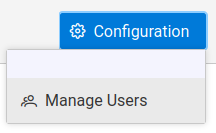
\includegraphics[width=0.25\textwidth]{imaxes/gestion-usuarios-01.png}
  \caption{Acceso a la pantalla de gestión de usuarios}
  \label{fig:boton-gestion-usuarios}
\end{figure}


Cada usuario tendrá asociado un perfil que define los permisos que tiene sobre la aplicación:
\begin{itemize}
\item \textbf{ADMIN} - permisos de administrador. Los usuarios con este perfil puede realizar altas, bajas y modificaciones de cualquier entidad de la aplicación: elementos de la parametrización, del catálogo, de la contratación o los usuarios del sistema.
\item \textbf{ADMIN} - permisos de lectura/escritura. Los usuarios con este perfil puede realizar altas, bajas y modificaciones de las entidades del catálogo del servicio, así como de las contrataciones, y únicamente consultar las entidades de la parametrización. No tienen habilitado el acceso a la gestión de usuarios.
\item \textbf{READ} - permisos de solo lectura. Los usuarios con este perfil sólo pueden consultar los datos de la aplicación correspondientes a la parametriación, el catálogo o la contratación. No tienen habilitado el acceso a la gestión de usuarios.
\end{itemize}


Una vez seleccionado se nos mostrará el listado de todos los usuarios del sistema (\figurename~\ref{fig:listado-usuarios}).
Desde ahí se pueden gestionar las siguientes operaciones:
\begin{description}
\item[\underline{\textsl{\textbf{Crear nuevo usuario}}}] Para crear un nuevo usuario se pulsará el botón \emph{New Data} situado en la parte superior de la tabla. Aparecerá una ventana emergente que mostrará un formulario con los campos a cubrir, entre ellos el perfil con el que se va a crear el usuario y que definirá los permisos de este sobre los elementos de la aplicación.

\item[\underline{\textsl{\textbf{Editar usuario}}}] Para editar un usuario se seleccionará del listado y se pulsará el botón editar de la columna \emph{EDIT ROW}. Se editarán los campos pertinentes de la tabla para realizar las modificaciones oportunas. 

\item[\underline{\textsl{\textbf{Borrar usuario}}}] Para borrar un usuario se seleccionará del listado y se pulsará el botón amarillo de borrar de la columna \emph{DEL ROW} correspondiente.
\end{description}


\begin{figure}[H]
  \centering
  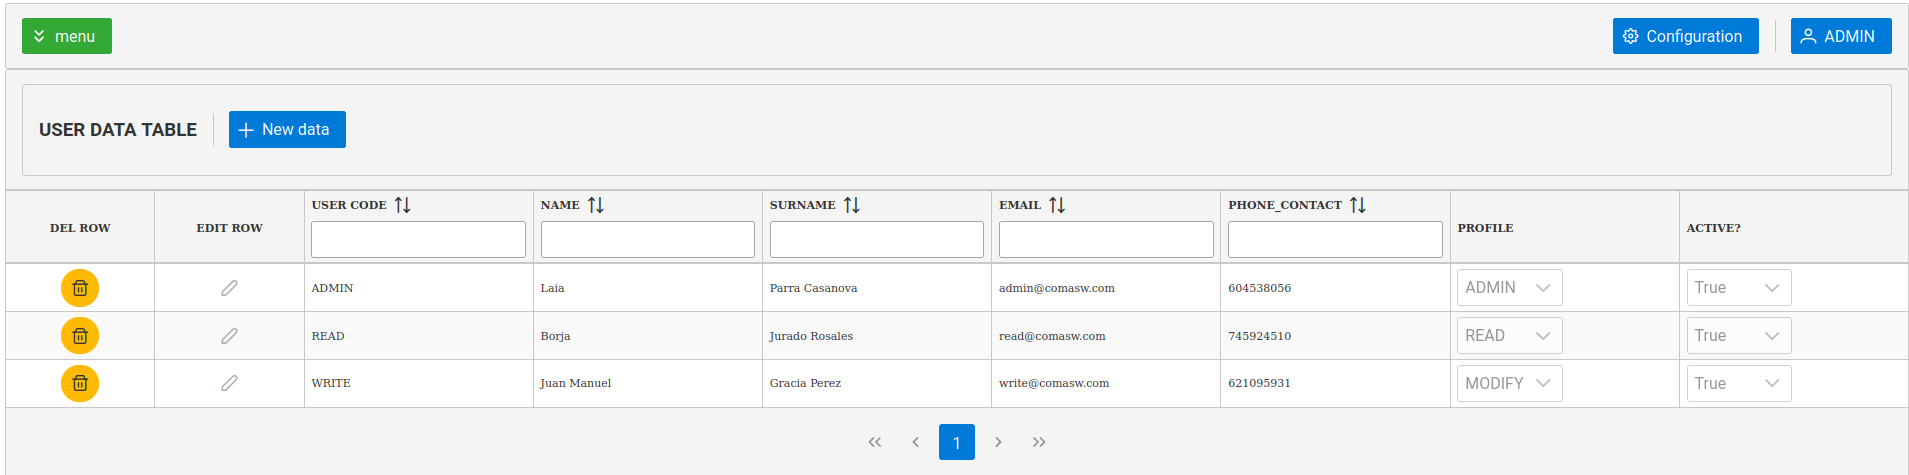
\includegraphics[width=\textwidth]{imaxes/gestion-usuarios-02.png}
  \caption{Listado de usuarios}
  \label{fig:listado-usuarios}
\end{figure}



\section{Manual de usuario}
\label{sec:manual-usuario}

En esta sección se mostrará toda la información necesaria para conocer el funcionamiento por parte del usuario de CoMaSw.


\subsection{Introducción}
\label{sub:introduccion}

Antes de explicar cómo usar \emph{CoMaSw} veamos la visión de contratación que propone la aplicación y los elementos que la conforman.



\subsubsection{Conceptos relativos a las contrataciones}
\label{sub:contratacion-conceptos}

Una contratación es una estructura jerárquica en la que el que la \textit{cabeza} de la misma es el cliente. Dicho cliente puede tener una o más cuentas asociadas. Cada una de estas cuentas es responsable de la contratación de un conjunto de productos, servicios, cuotas y promociones ofertados por la empresa. La \figurename~\ref{fig:estructura-contratacion} muestra dicha estructura de contratación. Vamos a introducir algunos conceptos al respecto.

\begin{figure}
  \centering
  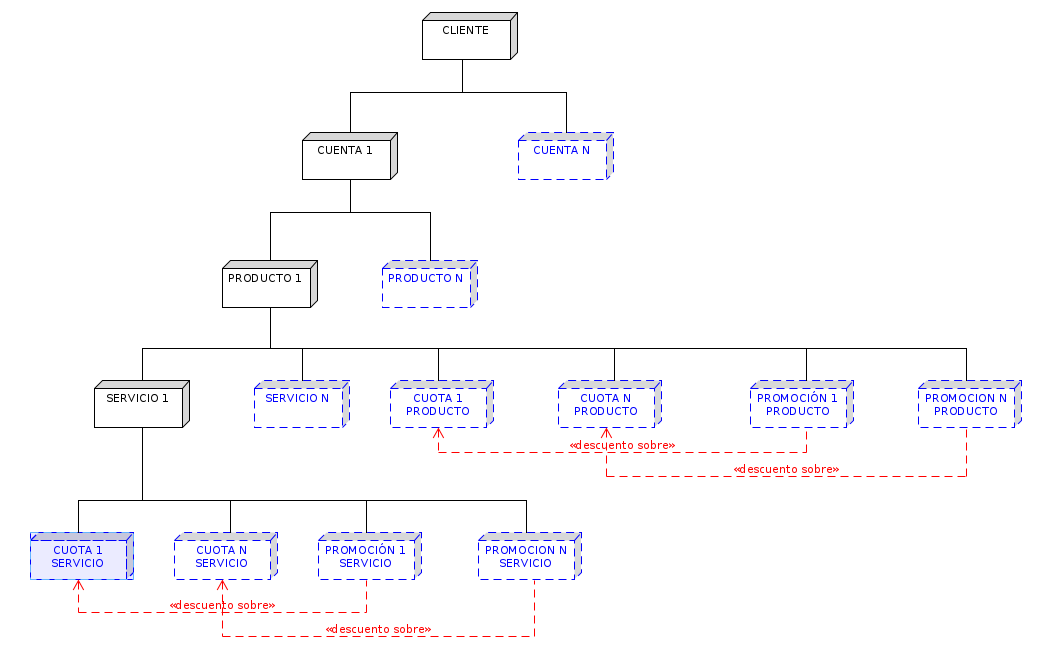
\includegraphics[width=\textwidth]{imaxes/estructura-contratacion.png}
  \caption{Estructura de la contratación}
  \label{fig:estructura-contratacion}
\end{figure}

\paragraph{Cliente.} Por cliente entendemos la persona física (particular o autónomo) o persona jurídica que adquiere los bienes y servicios proporcionados por la empresa a cambio de una transacción monetaria. Es el responsable último de la contratación de los servicios.

\paragraph{Cuenta.} Por cuenta entendemos la entidad del sistema que permite gestionar los distintos productos y servicios contratados por el cliente y es la responsable de la transacción económica asociada a la contratación, esto es, el \textit{pagador}, por lo que tendrá asociada una persona física o jurídica que es la que efectuará el pago y que puede coincidir con el cliente o ser otra distinta. Por lo tanto el ciclo de facturación que aplicará sobre los distintos elementos contratados vendrá dado por la cuenta asociada a los mismos.

\paragraph{Entidad facturable.} Por entidad facturable entendemos todo aquel elemento del sistema susceptible de generar un cargo facturable, y por lo tanto ha de tener un tipo impositivo asociado a la generación de estos cargos, de acuerdo con la ley vigente. Los cargos facturables se denomina elementos facturables y se clasifican en dos tipos:
\begin{itemize}
	\item \emph{\textbf{Cuotas}}: son los elementos que definen los cargos fijos a aplicar sobre las distintas entidades contratadas. Puede tratarse de un cargo que se emite una única vez durante el ciclo de vida de la entidad facturable (por ejemplo la cuota de alta) o cargos periódicos asociados a la prestación de servicios (por ejemplo la cuota mensual).
	\begin{itemize}
		\item Al hablar de cuotas aparece el concepto de \textbf{prorrateable}. Una cuota prorrateable es aquella para la que a la hora de calcular el cargo asociado a la misma durante la facturación se tiene en cuenta el tiempo en el que ha estado vigente dicha cuota: 
		\begin{itemize}
			\item si ha estado en vigencia durante todo el período de facturación se 		facturará el importe completo de la misma.
			\item si ha estado en vigencia sólo una parte del período de facturación se facturará la parte correspondiente a esa vigencia. 
		\end{itemize}
	\end{itemize}
	\item \emph{\textbf{Consumos}}: son los elementos que definen los cargos asociados a los distintos consumos que puede realizar el cliente bajo demanda y que, a diferencia de las cuotas, son importes variables sujetos a la naturaleza de los mismos y al comportamiento propio del consumidor en la demanda de los bienes ofertados. Un ejemplo de este tipo de consumos serían las llamadas de teléfono no incluidas en ningún plan de descuento. El importe a facturar por las llamadas dependerá de varios factores como el número de llamadas realizadas por el cliente, la duración de las mismas o el día y hora a las que las realice.
\end{itemize}


\paragraph{Producto.} Un producto es una entidad facturable conformada por el conjunto de servicios facturables y los posibles descuentos a aplicar sobre los distintos elementos facturables. Es el \textit{paquete} que la empesa oferta a sus clientes. Los únicos elementos facturables que se pueden aplicar sobre este tipo de entidad son del tipo cuota, y por lo tanto los descuentos a aplicar sólo afectarán a dichos cargos facturables.

\paragraph{Servicio.} Un servicio es otra entidad facturable que representa el bien inmateriar que se le presta al cliente y que es el verdadero objetivo de la contratación. Sobre este tipo de entidad pueden aplicarse tanto cuotas como consumos  y por lo tanto los descuentos a aplicar pueden afectara ambos tipos de elementos facturables.

\paragraph{Promoción.} Se entiene por promoción aquella entidad encargada de aplicar los descuentos previamente definidos sobre los distintos elementos facturables.



\subsubsection{Conceptos relativos al catálogo}
\label{sub:catálogo-conceptos}


Para llevar a cabo las distintas contratacione deberemos saber qué características puede tener cada uno de los elementos que intervienen y elegir unas u otras en función de las necesidades que presenta el cliente. Estas características vienen definidas por unas entidades \textit{plantillas} denominadas tipos que se encuentran englobadas dentro de lo que damos en denominar catálogo. En la \figurename~\ref{fig:estructura-catalogo} se muestra la estructura que define el catálogo de servicios de la aplicación y su implementación en una contratación de los mismos.

\begin{figure}[H]
  \centering
  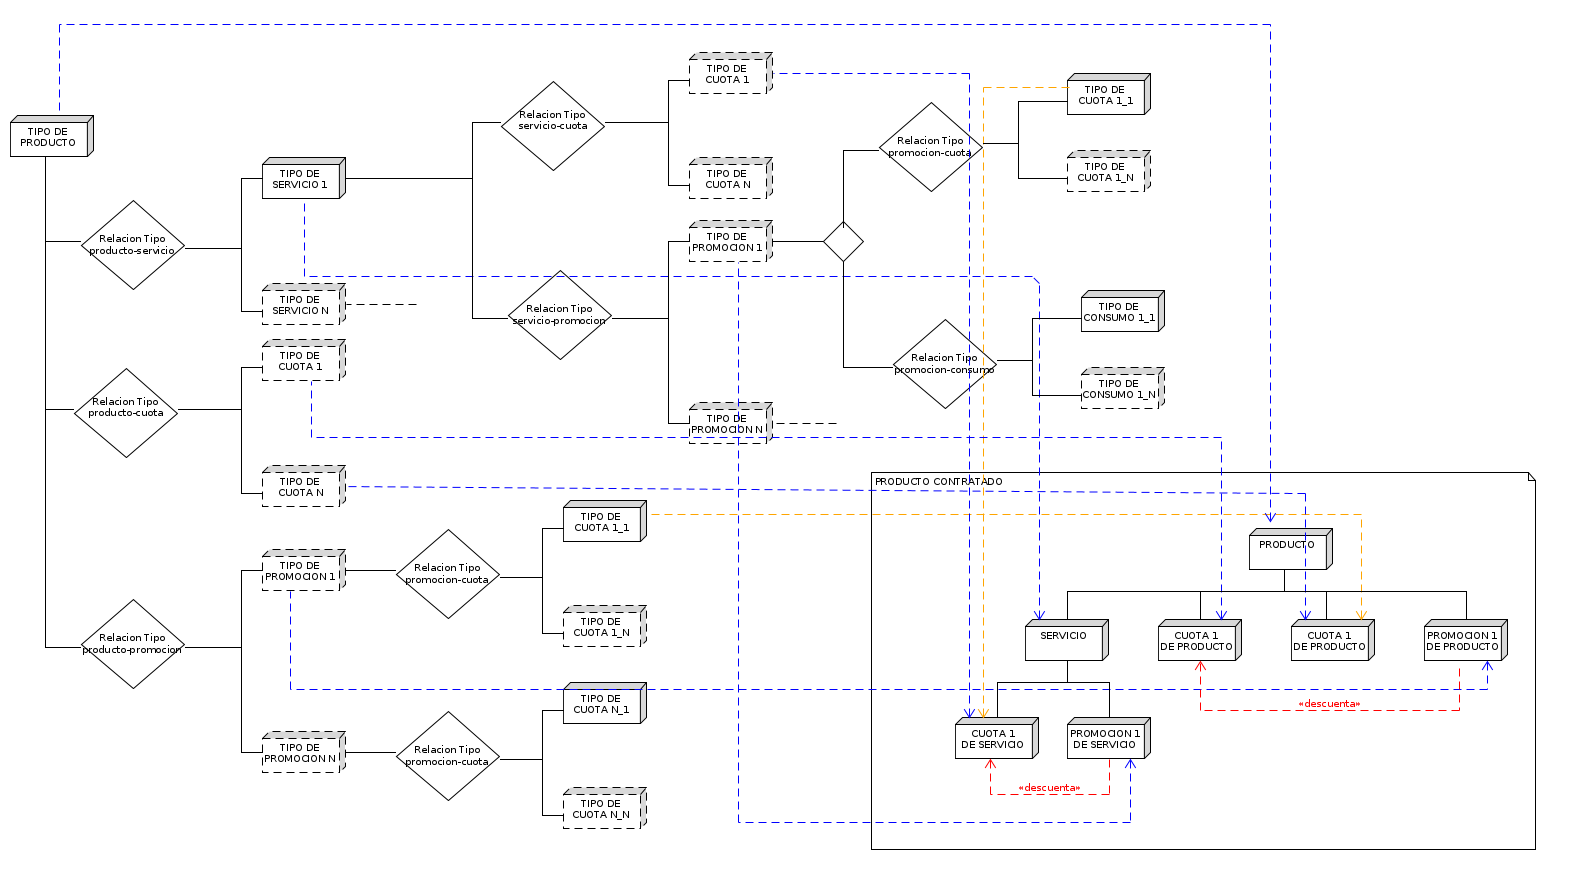
\includegraphics[width=\textwidth]{imaxes/estructura-catalogo.png}
  \caption{Estructura del catálogo de servicios y su implementación en una contratación}
  \label{fig:estructura-catalogo}
\end{figure}


El catálogo de la aplicación define los distintos elementos que conforman el catálogo de servicios así como otras entidades que permiten definir las instancias finales de contratación.



En la sección \ref{sec:manual-usuario} de la página \pageref{sec:manual-usuario} veremos cómo definir todos estos elementos y alguno más con el fin de disponer de una herramienta de contratación plenamente funcional.



\subsubsection{Conceptos relativos a los registros de histórico}
\label{sub:histórico-conceptos}

Puesto que los elementos que conforman las contrataciones son suceptibles de sufrir modificaciones durante su ciclo de vida (nuevas altas de productos, modificación en el precio de las cuotas, expiración de promociones, etc.) todas estas entidades están conformadas por un conjunto de registros históricos que contienen la \textit{foto} de la contratación para el período temporal indicado por las fechas incio y fin de dicho registro. Lo mismo ocurre con los elementos del catálogo que también pueden sufrir modificaciones en sus condiciones de aplicación, como son las definiciones de cuotas y promociones.

En todos estos casos los registros deben ser consecutivos en el tiempo, para lo que se define una serie de limitaciones a tener en cuenta a la hora de manejar los distintos registros de histórico. Por lo tanto, dado el total de registros de histórico para una determinada entidad ordenados de forma cronólogica, desde la menor fecha de inicio a la mayor, estos registros deberán cumplir con las siguientes condiciones:
\begin{itemize}
\item Si existen varios registros en el sistema para una entidad dada, la fecha de inicio de cada uno de ellos deberá ser igual a la fecha  de finalización del registro inmediatamente anterior más un día, salvo para el primero de los registros de histórico.
	\item Si existen varios registros en el sistema para una entidad dada, la fecha de fin de cada uno de ellos deberá ser igual a la fecha  de inicio del registro inmediatamente anterior menos un día, salvo para el último de los registros de histórico.
	\item Si queremos \textit{partir} un registro existente para introducir un nuevo registro de histórico se modificarán las fechas de inicio y fin del registro existente para adaptarlo a las condiciones indicadas en los dos puntos anteriores, de tal forma que:
	\begin{itemize}
		\item Si la fecha de inicio del nuevo registro a insertar coincide con la fecha de inicio del nuevo registro a insertar, se modificará la fecha de inicio del registro existente a la fecha de fin del nuevo registro más un día, por lo que en este caso debe haber un \uline{margen de al menos un día entre la fecha de inicio y la fecha fin del registro existente} que se desea partir. 
		\item Si la fecha de fin del nuevo registro a insertar coincide con la fecha de fin del nuevo registro a insertar, se modificará la fecha de fin del registro existente a la fecha de inicio del nuevo registro menos un día, por lo que en este caso debe haber un \uline{margen de al menos un día entre la fecha de inicio y la fecha fin del registro existente} que se desea partir. 
		\item Si las fechas de inicio y fin del nuevo registro a insertar están comprendidas dentro de las fechas de inicio y fin del registro existente, pero no coinciden con éstas, a partir del registro existente se creará una copia del registro con la misma información que el registro existente de tal forma que la fecha de fin del registro existente será la fecha de inicio menos un día del nuevo registro y la fecha de inicio del registro copiado será la fecha de fin del nuevo registro más un día, por lo que en este caso debe haber un \uline{margen de al menos un día entre la fecha de inicio del registro existente y la fecha de inicio del nuevo registro} y  \uline{otro margen de al menos un día entre la fecha de fin del nuevo registro y la fecha de fin del registro existente}.
	\end{itemize}
	\item Si se borra un registro de histórico intermedio, la fecha de fin del registro anterior al registro borrado se modificará a la fecha de fin del registro posterior al borrado menos un día. Si se borra el primer o el último elemento del histórico no se realiza ninguna modificación adicional sobre el resto de los registros de histórico.	
\end{itemize}


\subsubsection{Registro de operaciones en el sistema}
\label{sub:registro-operaciones}

La aplicación lleva a cabo un registro de las operaciones de edición sobre las entidades del sistema, de tal forma que:
\begin{itemize}
\item si se crea una nueva entidad, se registrará el usuario y la fecha en la que se realizó dicho alta.
\item si se modifica alguna entidad existente, se registrará el usuario y la fecha en la que se realizó dicha modificación sobre la entidad. Para el caso de las entidades con registro de histórico este registro se realizará sobre los registros de histórico afectados.
\end{itemize}



\subsection{Acceso}

Para acceder a la aplicación es necesario estar dado de alta y disponer de un
usuario y contraseña.

El administrador se encargará de proporcionarle un usuario y contraseña válidos para el acceso a la aplicación, así como la dirección web de acceso a la aplicación.

La aplicación utiliza usuarios para el control de acceso y para auditar la
modificación de la información almacenada. 

Una vez introducida la dirección web indicada por nuestro administrador, aparecerá una ventana con un formulario de acceso(\figurename~\ref{fig:login}). Introduciremos el usuario y la contraseña y pulsaremos aceptar. 


\begin{figure}[H]
  \centering
  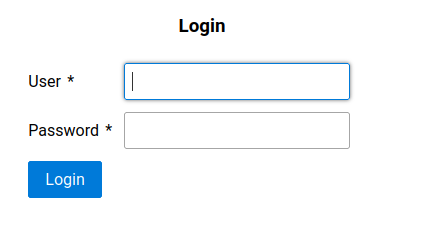
\includegraphics[width=0.40\textwidth]{imaxes/login.png}
  \caption{Pantalla de logado}
  \label{fig:login}
\end{figure}

Si los datos introducidos son correctos se mostrará la página de inicio de la aplicación.

Para salir de la aplicación pulsaremos el botón con nuestro nombre de usuario situado en la esquina superior derecha y seleccionaremos la opción logout (ver \figurename~\ref{fig:logout}). Una vez pulsado se cierra la sesión y la aplicación nos redirige a la pantalla de inicio de sesión.

\begin{figure}[H]
  \centering
  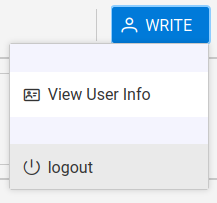
\includegraphics[width=0.25\textwidth]{imaxes/logout.png}
  \caption{Logout}
  \label{fig:logout}
\end{figure}


\subsection{Cambio de contraseña y/o datos de contacto de un usuario}
\label{sub:contraseña}
Un usuario puede modificar tanto su contraseña de acceso como los datos relativos a su ficha. Para ello pulsará el botón de la esquina superior derecha con su nombre de usuario y seleccionará la opción \textit{View User Info} .
Se mostrará una pantalla con un botón para cambiar la contraseña así como un área con los datos del usuario y un botón para editar la información.

\begin{description}
\item[\underline{\textsl{Modificar contraseña}}] Se pulsará el botón \emph{Change Password}. Aparecerán dos campos editables para introducir la nueva contraseña a cambiar y un botón para guardar los cambios. Los valores introducidos en ambos campos deberán ser iguales. En caso contrario la aplicación mostrará un error de validación y no se modificará la contraseña.

\item[\underline{\textsl{Editar información del usuario}}] Pulsando el botón \emph{Edit Data} se habilitará la edición de los campos con la información del usuario y un botón para guardar los cambios.
\end{description}


\subsection{Acceder al menú de la aplicación}
\label{sub:menu}
Pulsando el botón \emph{Menu} de la esquina superior izquierda se despliega el menú de la aplicación (\figurename~\ref{fig:menu}).

\begin{figure}[H]
  \centering
  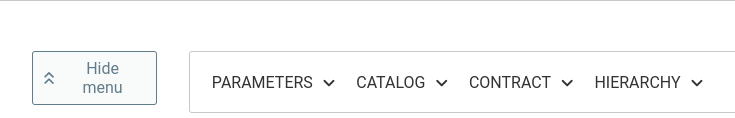
\includegraphics[width=0.6\textwidth]{imaxes/menu-aplicacion.png}
  \caption{Detalle del menú de la aplicación}
  \label{fig:menu}
\end{figure}

El menú se divide en cuatro bloques:
\begin{itemize}
\item \emph{\textbf{PARAMETERS}}: da acceso a las distintas entidades de parametrización, necesarias para la definición del resto de entidades de la aplicación.
\item \emph{\textbf{CATALOG}}: da acceso a las distintas entidades del catálogo de servicios de la aplicación.
\item \emph{\textbf{CONTRACT}}: da acceso a las distintas entidades de contratación de la aplicación.
\item \emph{\textbf{HIERARCHY}}: da acceso a la ventana de visualización jerárquica de las contrataciones.
\end{itemize}

El botón que se encuentra más a la izquierda, fuera del área del menú, permite ocultar la ventana emergente del menú.


A continuación entraremos en detalle en cada uno de estos apartados.

\subsection{Parametrización}
\label{sub:parametrizacion}

Con idea de hacer lo más flexible y adaptable posible esta aplicación, se han definido una serie de elementos de parametrización para la definición de las distintas entidades de la aplicación. En la \tablename~\ref{tab:parametrizacion} se puede consultar un listado de los elementos de parametrización existentes en la aplicación. Para acceder a cada una de estas entidades se desplegará la sección \emph{PARAMETERS} del menú principal y se seleccionará el tipo de entidad correspondiente del listado desplegado.



\begin{table}[H]
  \centering
  \rowcolors{2}{white}{udcgray!25}
  \setlength{\leftmargini}{0.4cm}
  \resizebox{14cm}{!} {
  \begin{tabular}{|m{4cm} m{11cm}|}
  \rowcolor{udcpink!25}
  \hline
  	\textbf{Elemento} & \textbf{Descripción} \\\hline
	\textbf{Entity Types} & Listado de entidades contempladas en el sistema. Son siete, correspondientes a producto, servicio, cuota, consumo, promoción, cliente y cuenta.   \\
	\textbf{Consumption Classes} & Clases de consumos definidos. Actualmente hay cuatro correspondientes a llamada, SMS, MMS y Datos. Necesario para definir los consumos definidos en el catálogo. \\
	\textbf{Status} & Estados permitidos dentro del sistema para las entidades del catálogo y la contratación.. Se definen dos ámbitos de aplicación: para las entidades del catálogo y/o para las de la contratación. Un mismo estado puede ser compartido por entidades de distinto ámbito. \\
	\textbf{Application Level} & Define el nivel de aplicación de las cuotas y las promociones. Actualmente hay dos niveles definidos: producto y servicio.  \\
	\textbf{Discount Type} & Tipos de descuento existentes en la aplicación. Usados para definir las promociones. Actualmente hay cuatro tipos: (volumen de) Megabytes, (volumen de) minutos, unidades (número de sms) y porcentaje (a descontar sobre el total facturado).   \\
	\textbf{Payment Method} & Métodos de pago. Se usa a la hora de instanciar una cuenta (contratación) pra definir el método de pago de ese cliente. \\
Billing Period & Los distintos períodos de facturación definidos. Usado para definir los distintos tipos de facturación. \\
	\textbf{Tax Type} & Tipo impositivo. Usado durante la contratación de un producto o servicio, para definir el tipo impositivo que se debe aplicar sobre el mismo de cara a la facturación.\\
	\textbf{Identity Card Type} & Tipo de documento de identificación (NIF, NIE, Pasaporte).
	\\\hline
  \end{tabular}
  } % end /resizebox
  \caption{Entidades de Parametrizacion}
  \label{tab:parametrizacion}
\end{table}

La gestión de estas entidades no está disponible para todos los usuarios, tal y como se muestra en la \figurename~\ref{fig:parametrizacion}). Sólo los usuarios con permisos de administrador de la aplicación podrán añadir, editar o borrar elementos, habilitándoseles los correspondientes botones para dichas operaciones (\figurename~\ref{fig:parametrizacion-admin}). Para el resto de usuarios sólo se mostrará el listado de dichos elementos (\figurename~\ref{fig:parametrizacion-usuario}).


\begin{figure}[H]
  \centering
  \begin{subfigure}[c]{\textwidth}
    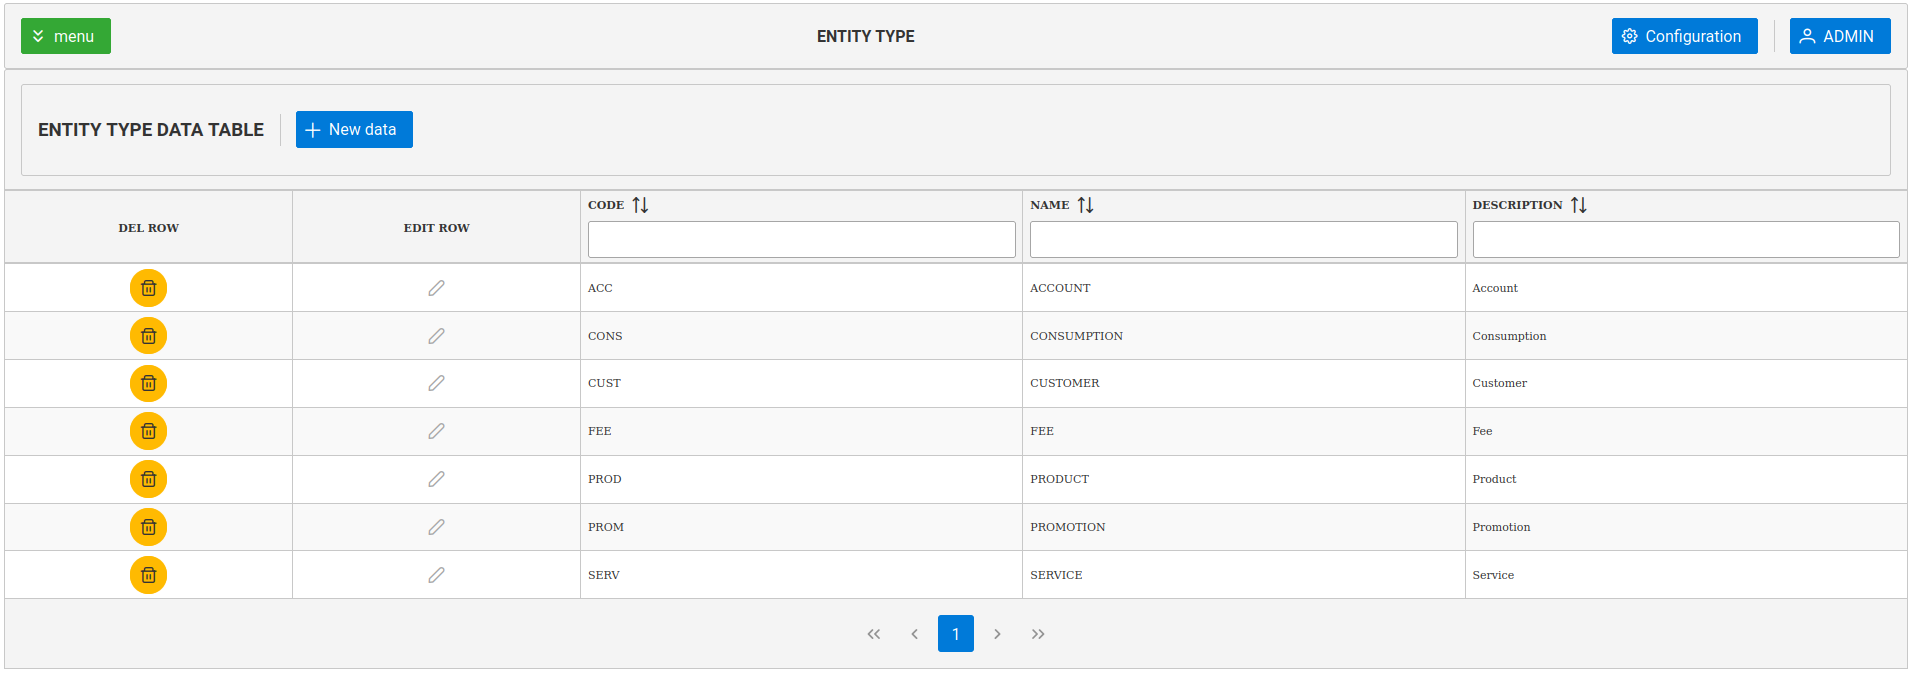
\includegraphics[width=\textwidth]{imaxes/entity-type-admin.png}
    \caption{Vista de la pantalla Entity Types para usuarios con perfil de administrador\newline}
    \label{fig:parametrizacion-admin}
  \end{subfigure}
  \begin{subfigure}[c]{\textwidth}
    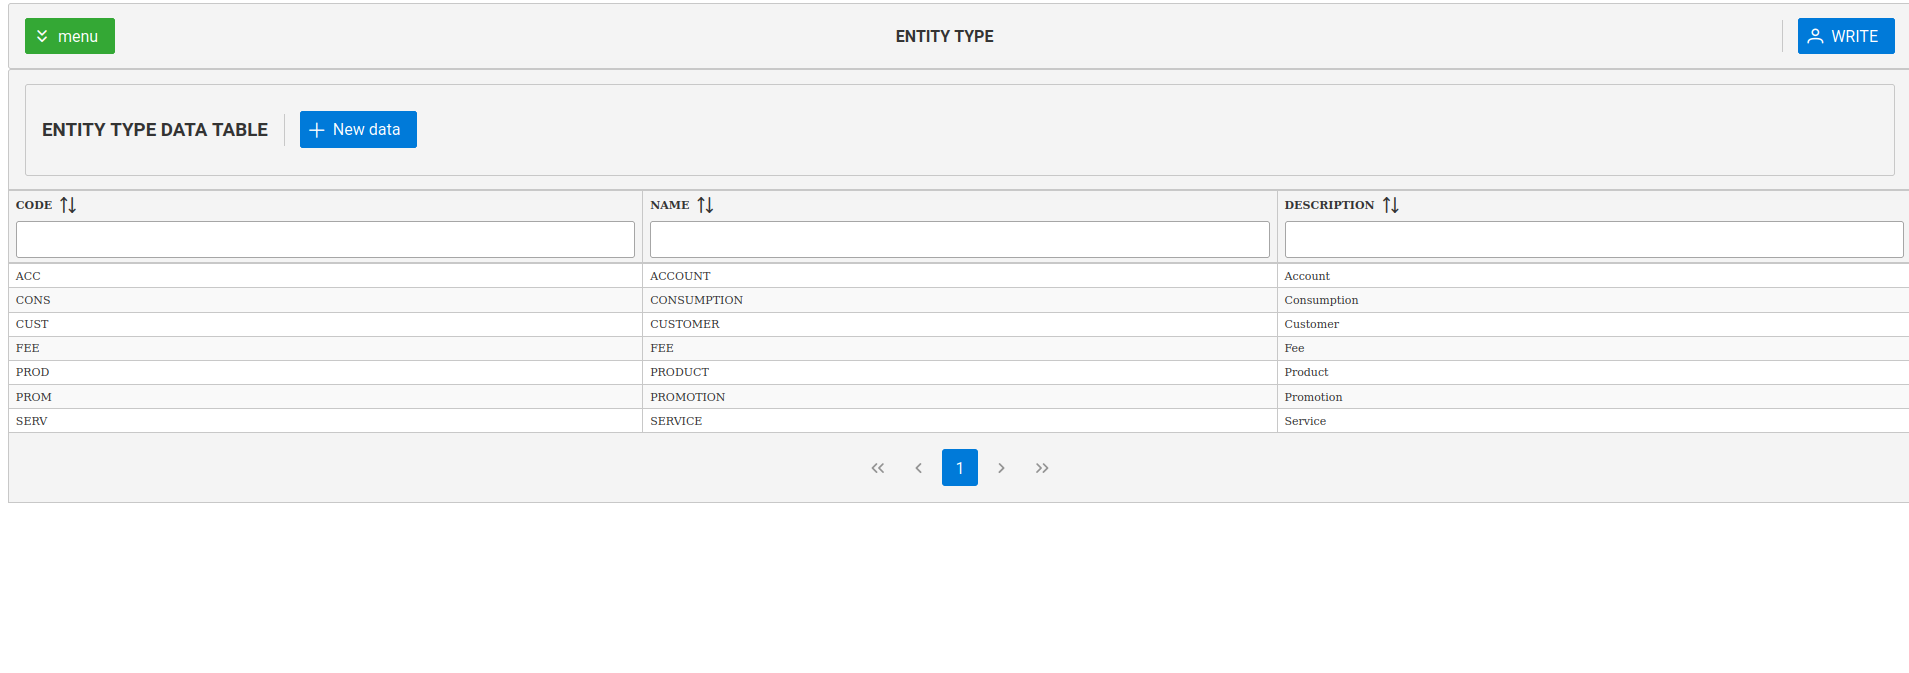
\includegraphics[width=\textwidth,height=3cm]{imaxes/entity-type-usuario.png}
    \caption{Vista de la pantalla Entity Types para el resto de perfiles de usuario}
    \label{fig:parametrizacion-usuario}
  \end{subfigure}
  \caption{Comparativa de las vistas de la pantalla Entity Types según los permisos del usuario.}
  \label{fig:parametrizacion}
\end{figure}

Para los usuarios con perfil de administrador se definen las siguients operaciones, siendo \textit{entidad} el tipo de elemto al que hemos accedido a través del menú. El funcionamiento es el mismo para todas las entidades, sólo cambia la información a almacenar, que vendrá dada por la naturaleza de la misma.

\begin{description}
\item[\underline{\textsl{\textbf{Crear nueva entidad}}}] Para crear una nueva entidad se pulsará el botón \textit{New Data} situado en la parte superior de la tabla. Aparecerá una ventana emergente que mostrará un formulario con los campos a cubrir.

\item[\underline{\textsl{\textbf{Editar entidad existente}}}] Para editar una entidad se seleccionará del listado y se pulsará el botón editar de la columna \textit{EDIT ROW} correspondiente. Se editarán los campos pertinentes directamente en la tabla para realizar las modificaciones oportunas. 

\item[\underline{\textsl{\textbf{Borrar entidad}}}] Para borrar una entidad se seleccionará del listado y se pulsará el botón amarillo de borrar de la columna \textit{DEL ROW} correspondiente.
\end{description}

Todos los valores mostrados para la entidad son obligatorios y deberán cubrirse al realizar un alta o modificación. Asimismo el valor del campo CODE es único. No pueden existir dos entidades del mismo tipo con el mismo código.


\subsection{Catálogo}
\label{sub:catálogo}

El catálogo del sistema está formado por las distintas definiciones de productos, servicios, cuotas, consumos y promociones que ofrece la empresa y las relaciones que guardan entre sí. A estas definiciones les hemos dado en llamar tipos (\textit{type}).

Además de estas seis entidades indicadas, hemos incluido en esta clasificación otras entidades, que si bien no forman parte del catálogo de servicios de una empresa propiamente dicho, sí son definiciones de entidades que nos ayudarán a clasificar los datos a la hora de realizar contrataciones.


Todos los usuarios del sistema tienen acceso a los elementos del catálogo, pero aquellos que tengan permisos de edición (perfil ADMIN o MODIF) podrán gestionarlos (realizar altas, bajas y modificaciones). Los usuarios con el perfil READ sólo podrán acceder en modo consulta, y no se mostrarán habilitados los correspondientes botones para las operaciones de gestión. Por comodidad las imágenes que proceden a ilustrar esta sección se corresponderán con el acceso a las vistas de un usuario con permisos de edición. Los usuarios sin estos permisos verán la misma pantalla pero sin los botones que permiten la gestión de los datos.


Se definen tres estados distintos para las entidades del catálogo:
\begin{description}
\item[ACTIVE] Estado activo. Para las entidades del catálogo que están disponibles para ofertar.
\item[DEVELOP] Estado \textit{en desarrollo}. Para las entidades del catálogo que todavía no están disponibles para ofertar.
\item[CANCEL] Estado cancelado. Para las entidades del catálogo que están disponibles para ofertar.
\end{description}



A continuación detallaremos cada una de estas entidades a las que accederemos a través del menú \emph{CATALOG}.

\subsubsection{Bill Cycle Type - Tipo de ciclo de facturación}
\label{sub:billcycle}

Nota: Para acceder a la pantalla que da acceso a la operativa de este tipo de entidad se desplegará la sección \emph{CATALOG} del menú principal y se seleccionará el tipo de entidad \emph{Bill Cycle Type}.

La facturación escapa del ámbito de esta aplicación. Sin embargo toda contratación de servicios tiene como fin último monetizar la prestación de un servicio, por lo que la información del ciclo de facturación en el que va a entrar un elemento contratado es un factor a tener en cuenta a la hora de de realizar las contrataciones.

Un tipo de ciclo de facturación viene definido por los elementos indicados en la \tablename~\ref{tab:ciclo-facturacion}:



\begin{table}[H]
  \centering
  \rowcolors{2}{white}{udcgray!25}
  \setlength{\leftmargini}{0.4cm}
  \resizebox{14cm}{!} {
  \begin{tabular}{|m{3.5cm} m{11cm}|}
  \rowcolor{udcpink!25}
  \hline
  	\textbf{Elemento} & \textbf{Descripción} \\\hline
	\textbf{CODE} & Código identificativo del ciclo de facturación. Es único.   \\
	\textbf{NAME} & Nombre del ciclo del facturador. \\
	\textbf{DESCRIPTION} & Descripción del ciclo de facturador. \\
	\textbf{CORRECTIVE} & Valor \emph{True} indica que estamos ante un ciclo de facturación correctivo (a aplicar en refacturaciones). En caso contrario estaremos ante un ciclo de facturación ordinario (el que se ejecuta períodicamente)\\
	\textbf{BILLING PERIOD} & Período de facturación definido para el ciclo de facturación. Se corresponde con los períodos de facturación definidos en la correspondiente entidad de \emph{PARAMETERS} definida en la sección \ref{sub:parametrizacion}.   \\
	\textbf{BILL CYCLE DAY} & Día en el que se inicia un período de facturación. \\
	\textbf{CODENUM} & Código alfanumérico que identifica el número de la factura.\\
	\textbf{STATUS} & Estado del ciclo de facturación.
	\\\hline
  \end{tabular}
  } % end /resizebox
  \caption{Datos que definen el ciclo de facturación.}
  \label{tab:ciclo-facturacion}
\end{table}


Las operaciones definidas para esta entidad son las siguientes (nota: sólo están habilitadas para usuarios con permisos de edición):
\begin{description}
  \item[\underline{\textsl{\textbf{Crear nuevo tipo de ciclo de facturación}}}] Para crear un nuevo tipo ciclo de facturación se pulsará el botón \textit{New Data} situado en la parte superior de la tabla. Aparecerá una ventana emergente que mostrará un formulario con los campos a cubrir.

  \item[\underline{\textsl{\textbf{Editar tipo de ciclo de facturación existente}}}] Para editar un tipo de ciclo de facturación existente se seleccionará del listado y se pulsará el botón editar de la columna \textit{EDIT ROW} correspondiente. Se editarán los campos pertinentes directamente en la tabla para realizar las modificaciones oportunas. 

  \item[\underline{\textsl{\textbf{Borrar ciclo de facturación}}}] Para borrar un tipo de ciclo de facturación se seleccionará del listado y se pulsará el botón amarillo de borrar de la columna \textit{DEL ROW} correspondiente.
\end{description}

Todos los valores mostrados para la entidad son obligatorios y deberán cubrirse al realizar un alta o modificación. Asimismo el valor del campo CODE es único. No pueden existir dos entidades del mismo tipo con el mismo código.



\subsubsection{Customer Type - Tipo de cliente}
\label{sub:customer-type}

Nota: Para acceder a la pantalla que da acceso a la operativa de este tipo de entidad se desplegará la sección \emph{CATALOG} del menú principal y se seleccionará el tipo de entidad \emph{Customer Type}.

En este apartado nos centraremos en la gestión de los tipos de cliente, que permiten clasificar los distintos clientes de la cartera de clientes existentes en el sistema.


Un tipo de cliente viene definido por los elementos indicados en la \tablename~\ref{tab:tipo-cliente}:



\begin{table}[H]
  \centering
  \rowcolors{2}{white}{udcgray!25}
  \setlength{\leftmargini}{0.4cm}
  \resizebox{14cm}{!} {
  \begin{tabular}{|m{3cm} m{11cm}|}
  \rowcolor{udcpink!25}
  \hline
  	\textbf{Elemento} & \textbf{Descripción} \\\hline
	\textbf{CODE} & Código identificativo del tipo del cliente. Es único.   \\
	\textbf{NAME} & Nombre del tipo del cliente. \\
	\textbf{DESCRIPTION} & Descripción del tipo de cliente. \\	
	\textbf{STATUS} & Estado del tipo de cliente.
	\\\hline
  \end{tabular}
  } % end /resizebox
  \caption{Datos que define un tipo de cliente.}
  \label{tab:tipo-cliente}
\end{table}

Las operaciones definidas para esta entidad son las siguientes (nota: sólo están habilitadas para usuarios con permisos de edición):
\begin{description}
\item[\underline{\textsl{\textbf{Crear nuevo tipo de cliente}}}] Para crear un nuevo cliente se pulsará el botón \textit{New Data} situado en la parte superior de la tabla. Aparecerá una ventana emergente que mostrará un formulario con los campos a cubrir.

\item[\underline{\textsl{\textbf{Editar tipo de cliente existente}}}] Para editar un tipo de cliente existente se seleccionará del listado y se pulsará el botón editar de la columna \textit{EDIT ROW} correspondiente. Se editarán los campos pertinentes directamente en la tabla para realizar las modificaciones oportunas. 

\item[\underline{\textsl{\textbf{Borrar tipo de cliente}}}] Para borrar un tipo de cliente se seleccionará del listado y se pulsará el botón amarillo de borrar de la columna \textit{DEL ROW} correspondiente.
\end{description}

Todos los valores mostrados para la entidad son obligatorios y deberán cubrirse al realizar un alta o modificación. Asimismo el valor del campo CODE es único. No pueden existir dos entidades del mismo tipo con el mismo código.




\subsubsection{Account Type - tipo de cuenta}
\label{sub:account-type}

Nota: Para acceder a la pantalla que da acceso a la operativa de este tipo de entidad se desplegará la sección \emph{CATALOG} del menú principal y se seleccionará el tipo de entidad \emph{Customer Type}.

En este apartado nos centraremos en la gestión de los tipos de cuenta, que permiten clasificar las distintas cuentas de la cartera de clientes existentes en el sistema.

Una cuenta es la entidad que alberga el conjunto de elementos contratados y es sobre la que se definen los datos de facturación. Un cliente puede tener varias cuentas en función de, por ejemplo, la ubicación en la que se encuentran los servicios contratados (por ejemplo una cuenta para la vivienda habitual y otra para la segunda residencia). 


Un tipo de cuenta viene definido por los elementos indicados en la \tablename~\ref{tab:tipo-cuenta}:



\begin{table}[H]
  \centering
  \rowcolors{2}{white}{udcgray!25}
  \setlength{\leftmargini}{0.4cm}
  \resizebox{14cm}{!} {
  \begin{tabular}{|m{4cm} m{11cm}|}
  \rowcolor{udcpink!25}
  \hline
  	\textbf{Elemento} & \textbf{Descripción} \\\hline
	\textbf{CODE} & Código identificativo del tipo de cuenta. Es único.   \\
	\textbf{NAME} & Nombre del tipo de cuenta. \\
	\textbf{DESCRIPTION} & Descripción del tipo de cuenta. \\	
	\textbf{PAYMENT METHOD} & Tipo de pago asociado a la cuenta. Se corresponde con los metodos de pago definidos en la correspondiente entidad de \emph{PARAMETERS} definida en la sección \ref{sub:parametrizacion}. \\	
	\textbf{ORDINARY CYCLE} & Tipo de ciclo de facturación ordinario especificado para este tipo de cuenta. Se corresponde los tipos de ciclo de factuarción definidos como ordiniarios de la entidad de catálogo \ref{sub:billcycle}. \\	 		\textbf{CORRECTIVE CYCLE} & Tipo de ciclo de facturación correctivo especificado para este tipo de cuenta. Se corresponde los tipos de ciclo de factuarción definidos como correctivos de la entidad de catálogo \ref{sub:billcycle}. \\	
	\textbf{STATUS} & Estado del tipo de la cuenta.
	\\\hline
  \end{tabular}
  } % end /resizebox
  \caption{Datos que define un tipo de cuenta.}
  \label{tab:tipo-cuenta}
\end{table}

Las operaciones definidas para esta entidad son las siguientes (nota: sólo están habilitadas para usuarios con permisos de edición):
\begin{description}
\item[\underline{\textsl{\textbf{Crear nuevo tipo de cuenta}}}] Para crear una nueva cuenta se pulsará el botón \textit{New Data} situado en la parte superior de la tabla. Aparecerá una ventana emergente que mostrará un formulario con los campos a cubrir.

\item[\underline{\textsl{\textbf{Editar tipo de cuenta existente}}}] Para editar un tipo de cuenta existente se seleccionará del listado y se pulsará el botón editar de la columna \textit{EDIT ROW} correspondiente. Se editarán los campos pertinentes directamente en la tabla para realizar las modificaciones oportunas.

\item[\underline{\textsl{\textbf{Borrar tipo de cuenta}}}] Para borrar un tipo de cuenta se seleccionará del listado y se pulsará el botón amarillo de borrar de la columna \textit{DEL ROW} correspondiente.
\end{description}

Todos los valores mostrados para la entidad son obligatorios y deberán cubrirse al realizar un alta o modificación. Asimismo el valor del campo CODE es único. No pueden existir dos entidades del mismo tipo con el mismo código.




\subsubsection{Consumption Type - tipo de consumo}
\label{sub:consumption-type}

Nota: Para acceder a la pantalla que da acceso a la operativa de este tipo de entidad se desplegará la sección \emph{CATALOG} del menú principal y se seleccionará el tipo de entidad \emph{Consumption Type}.

Consideramos los tipos de consumo como entidades perteneciente al catálogo de servicios propiamente dicho.

Como ya hemos indicado anteriormente, el importe a facturar por los consumos no puede saberse de antemano, ya que va ligada a los comportamientos a la hora de consumir esos elementos facturables. Sin embargo, puesto que como todo elemento facturable es susceptible de ser descontado por una promoción, deberemo guarda la definición de estos consumos.

Para simplificar su manejo nos hemos quedado con una definición lo más simple posible de este tipo de elementos facturables para poder establecer una relación entre estos elementos y los posibles descuentos a aplicar sobre los mismos. Por lo tanto se ignora lo relativo la información relativa a los costes asociados a los mismos, ya que esto está ligado a la definición de la tarificación de estos elementos facturables y consideramos que entra dentro del ámbito de un sistema de tarificación. 

Un tipo de consumo viene definido por los elementos indicados en la \tablename~\ref{tab:tipo-consumo}:



\begin{table}[H]
  \centering
  \rowcolors{2}{white}{udcgray!25}
  \setlength{\leftmargini}{0.4cm}
  \resizebox{14cm}{!} {
  \begin{tabular}{|m{3cm} m{11cm}|}
  \rowcolor{udcpink!25}
  \hline
  	\textbf{Elemento} & \textbf{Descripción} \\\hline
  	\textbf{CONSUMPTION CLASS} & Clase de consumo que estamos tratando. Las clases de consumo están definidas en la correspondiente entidad de \emph{PARAMETERS} definida en la sección \ref{sub:parametrizacion}.   \\
	\textbf{CODE} & Código identificativo del tipo de consumo. Es único.   \\
	\textbf{NAME} & Nombre del tipo de consumo. \\
	\textbf{DESCRIPTION} & Descripción del tipo de consumo. \\		
	\textbf{STATUS} & Estado del tipo del consumo.
	\\\hline
  \end{tabular}
  } % end /resizebox
  \caption{Datos que define un tipo de consumo.}
  \label{tab:tipo-consumo}
\end{table}

Las operaciones definidas para esta entidad son las siguientes (nota: sólo están habilitadas para usuarios con permisos de edición):
\begin{description}
\item[\underline{\textsl{\textbf{Crear nuevo tipo de consumo}}}] Para crear un nuevo consumo se pulsará el botón \textit{New Data} situado en la parte superior de la tabla. Aparecerá una ventana emergente que mostrará un formulario con los campos a cubrir.

\item[\underline{\textsl{\textbf{Editar tipo de consumo existente}}}] Para editar un tipo de consumo existente se seleccionará del listado y se pulsará el botón editar de la columna \textit{EDIT ROW} correspondiente. Se editarán los campos pertinentes directamente en la tabla para realizar las modificaciones oportunas.

\item[\underline{\textsl{\textbf{Borrar tipo de consumo}}}] Para borrar un tipo de consumo se seleccionará del listado y se pulsará el botón amarillo de borrar de la columna \textit{DEL ROW} correspondiente.
\end{description}

Todos los valores mostrados para la entidad son obligatorios y deberán cubrirse al realizar un alta o modificación. Asimismo el valor del campo CODE es único. No pueden existir dos entidades del mismo tipo con el mismo código.





\subsubsection{Fee Types - tipo de cuota}
\label{sub:fee-type}

Nota: Para acceder a la pantalla que da acceso a la operativa de este tipo de entidad se desplegará la sección \emph{CATALOG} del menú principal y se seleccionará el tipo de entidad \emph{Fee Types}.

Consideramos los tipos de cuotas como entidades pertenecientes al catálogo de servicios propiamente dicho.

A diferencia de los consumos, los cargos a facturar generados por las cuotas sí son conocidos de antemano y se definen dentro del catálogo de servicio.

Puesto que el importe de los cargos a facturar generados por las cuotas varían con el tiempo, se ha considerado la necesidad de llevar un registro de estos cambios a lo largo de la vida útil de este tipo de elementos. Por lo tanto una entidad de este tipo estará conformada por uno o varios registros con una fecha incio y una fecha fin que definen el período en el que aplican las condiciones definidas para esa entidad. Estos registros deben ser consecutivos de forma que si existen varios registros la fecha de inicio de un registro debe ser la fecha de fin del registro anterior mas un día (salvo para el primer registro que conforma el período del ciclo de vida del elemento). De igual forma la fecha de finalización de un registro debe ser la fecha de inicio del registro siguiente menos un día (salvo para el último registro que conforma el período del ciclo de vida del elemento).


Un tipo de cuota viene definido por los elementos indicados en la \tablename~\ref{tab:tipo-cuota}:




\begin{table}[H]
  \centering
  \rowcolors{2}{white}{udcgray!25}
  \setlength{\leftmargini}{0.4cm}
  \resizebox{14cm}{!} {
  \begin{tabular}{|m{3cm} m{11cm}|}
  \rowcolor{udcpink!25}
  \hline
  	\textbf{Elemento} & \textbf{Descripción} \\\hline
  	\textbf{START DATE} & Fecha de inicio del período temporal para el que aplican las condiciones especificadas para dicho período.\\
  	\textbf{END DATE} & Fecha de finalización del período temporal para el que aplican las condiciones especificadas para dicho período.\\
  	\textbf{CODE} & Código identificativo del tipo de cuota. Es único.\\
	\textbf{NAME} & Nombre del tipo de cuota.\\
	\textbf{DESCRIPTION} & Descripción del tipo de cuota.\\
	\textbf{APPLICATION LEVEL} & Nivel de aplicación de la cuota, esto es, a qué entidad facturable va asociado. Los niveles de aplicación están definidas en la correspondiente entidad de \emph{PARAMETERS} definida en la sección \ref{sub:parametrizacion}.\\	
	\textbf{PRORRATE} & Indica si la cuota es prorrateable (\textit{TRUE}) o no (\textit{FALSE}).\\
	\textbf{PRICE} & Indica el importe a facturar por dicha cuota.\\
	\textbf{STATUS} & Estado del tipo de cuota.	
	\\\hline
  \end{tabular}
  } % end /resizebox
  \caption{Datos que define un tipo de cuota.}
  \label{tab:tipo-cuota}
\end{table}



Las operaciones definidas para esta entidad son las siguientes:
\begin{description}
\item[\underline{\textsl{\textbf{Buscar un tipo de cuota existente}}}] Esta operación está disponible para todos los usuarios de la aplicación.

Puesto que los tipos de cuota son entidades con histórico, por motivos de operatividad no se muestra el listado de todas las entidades del sistema por defecto, si no que se establecen unos criterios de búsqueda para seleccionar el tipo de cuota a consultar. Para ello se define un área de búsqueda en los que se definen los criterios de búsqueda a tener en cuenta:
\begin{itemize}
\item Buscar todos los históricos de los tipos de consumo. Se realizará una búsqueda de todos los históricos de los distintos tipos de consumo.
\item Buscar por fecha. Se realizará una búsqueda de los históricos de todos los tipos de consumo existentes en el sistema para los que la fecha de búsqueda definida se encuentre entre la fecha de inicio y fin del registro de histórico. Opción marcada por defecto
\end{itemize}

Pulsando el botón \emph{Search} se mostrará un panel emergente con el listado de los registros encontrados. Seleccionaremos el elemento sobre el que queramos operar pulsando el botón amarillo de la columna \emph{Show Historic} (\figurename~\ref{fig:seleccion-tipo-cuota}):

\begin{figure}[H]
  \centering
  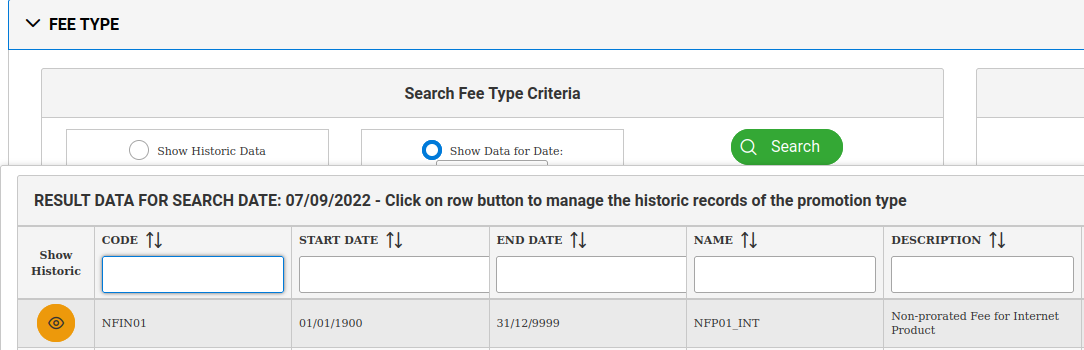
\includegraphics[width=0.90\textwidth]{imaxes/seleccion-tipo-cuota.png}
  \caption{Selección del tipo de cuota a modificar}
  \label{fig:seleccion-tipo-cuota}
\end{figure}


Se mostrará el área de históricos de la entidad con los distintos registros de histórico existentes (\figurename~\ref{fig:listado-historicos-tipo-cuota}):

\begin{figure}[H]
  \centering
  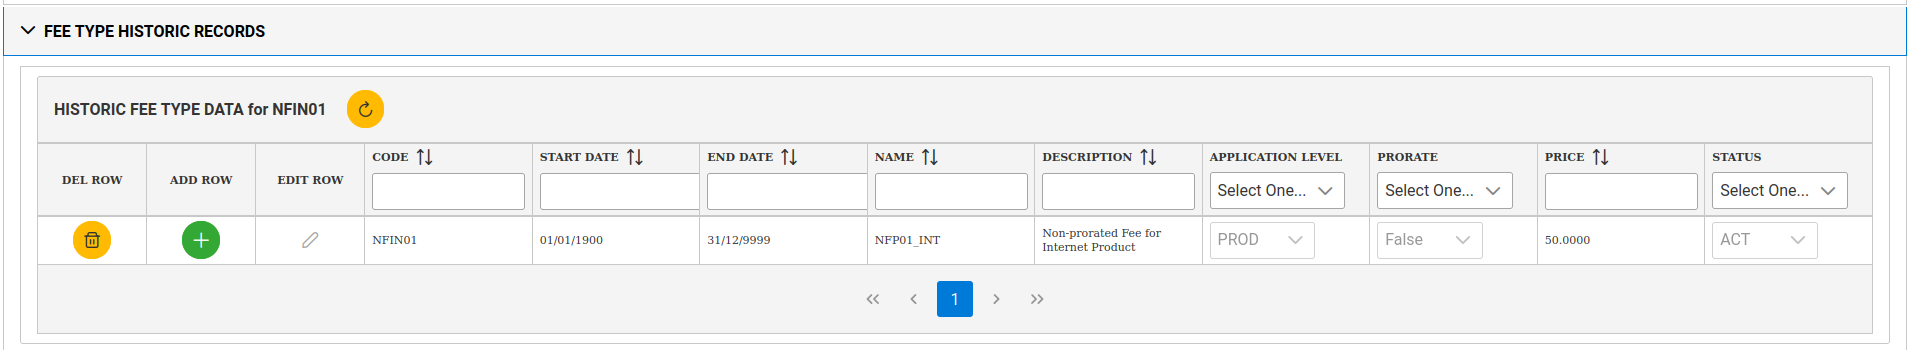
\includegraphics[width=\textwidth]{imaxes/listado-historicos-tipo-cuota.png}
  \caption{Listado de los históricos del tipo de cuota}
  \label{fig:listado-historicos-tipo-cuota}
\end{figure}


\item[\underline{\textsl{\textbf{Crear nuevo tipo de cuota}}}] Esta operación sólo está habilitada para usuarios con permisos de edición.
Para crear un nuevo consumo se pulsará el botón \textit{New Data} situado en la parte superior de la tabla. Aparecerá una ventana emergente que mostrará un formulario con los campos a cubrir. Por defecto se establecen como fecha de inicio y fin del nuevo tipo de cuota las fechas 01/01/1900 y 31/12/9999.

\item[\underline{\textsl{\textbf{Editar registro de histórico de un tipo de cuota existente}}}] Esta operación sólo está disponible para usuarios con permisos de edición.
Para editar un tipo de consumo existente se seleccionará del listado y se pulsará el botón editar de la columna \textit{EDIT ROW} correspondiente. Se editarán los campos pertinentes directamente en la tabla para realizar las modificaciones oportunas teniendo en cuenta los criterios de fechas establecidos (definidos en la sección \ref{sub:histórico-conceptos} de la página \pageref{sub:histórico-conceptos}).

\item[\underline{\textsl{\textbf{Añadir registro de histórico de un tipo de cuota existente}}}] Esta operación sólo está disponible para usuarios con permisos de edición.
Para añadir un nuevo registro de histórico sobre tipo de consumo existente se seleccionará del listado el registro en el que se ubicará el nuevo registro a añadir 
y se pulsará el botón añadir de la columna \textit{ADD ROW} correspondiente. Aparecerá una nueva ventana emergente como la que se muestra en la operación de creación, pero con los campos cubiertos con la información del registro sobre el que se va a añadir el nuevo registro y se realizán las moficaciones oportunas teniendo en cuenta los criterios de fechas establecidos (definidos en la sección \ref{sub:histórico-conceptos} de la página \pageref{sub:histórico-conceptos}).

\item[\underline{\textsl{\textbf{Borrar registro de histórico del tipo de cuota}}}] Esta operación sólo está disponible para usuarios con permisos de edición.
Para borrar un registro de histórico del tipo de consumo se seleccionará del listado el registro a borrar y se pulsará el botón amarillo de borrar de la columna \textit{DEL ROW} correspondiente.

\item[\underline{\textsl{\textbf{Borrar el tipo de cuota}}}] Esta operación sólo está disponible para usuarios con permisos de edición.
Para borrar completamente un tipo de cuota se deben borrar uno a uno todos los registros de histórico del tipo de cuota según lo indicado en el punto anterior. 

Todos los valores mostrados para la entidad son obligatorios y deberán cubrirse al realizar un alta o modificación. Asimismo el valor del campo CODE es único. No pueden existir dos entidades del mismo tipo con el mismo código.
\end{description}

A continuación describimos cómo proceder para realizar las distintas operaciones de modificación de un registro de histórico (edición de registro de histórico, añadir un nuevo registro de histórico y borrar un registro de histórico). Como paso previo a estas operaciones debermos haber buscado la entidad de tipo cuota a modificar:


\paragraph{Añadir un nuevo registro de histórico:} para ello seleccionamos el registro de histórico a modificar y pulsamos el botón verde \emph{ADD ROW}. Aparecerá una ventana emergente con un formulario de edición. Modificamos los datos correspondientes, por ejemplo la fecha inicio del nuevo registro y el importe de la cuota y pulsamos el botón azul \emph{OK} de confirmación (\figurename~\ref{fig:añadir-registro-historico-tipo-cuota}).

\begin{figure}
  \centering
  \includegraphics[width=0.45\textwidth]{imaxes/añadir-registro-historico-tipo-cuota.png}
  \caption{Formulario para añadir un nuevo registro de histórico del tipo de cuota}
  \label{fig:añadir-registro-historico-tipo-cuota}
\end{figure}


Una vez pulsado el botón de confirmación se cierra el formulario y se muestra la lista actualizada del registro de histórico con la nueva definición del tipo de consumo. Comprobamos que se ha modificado la fecha de incio del registro ya existente en el sistema y que figura el nuevo registro añadido con los correspondientes valores modificados, tal y como se muestra en la \figurename~\ref{fig:listado-historico-tipo-consumo-tras-añadir}.

\begin{figure}
  \centering
  \includegraphics[width=\textwidth]{imaxes/listado-historico-tipo-consumo-tras-añadir.png}
  \caption{Listado de registros de histórico tras la adición de un nuevo registro de histórico}
  \label{fig:listado-historico-tipo-consumo-tras-añadir}
\end{figure}


\paragraph{Borrar un registro de histórico:} para ello seleccionamos el registro de histórico a modificar y pulsamos el botón amarillo \emph{DEL ROW}, por ejemplo el registro añadido en el ejemplo anterior. Aparecerá un diálogo de confirmación indicando el período del registro a borrar, tal y como se muestra en la \figurename~\ref{fig:borrado-historico-tipo-cuota}.


\begin{figure}
  \centering
  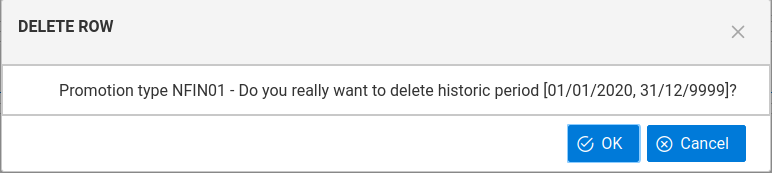
\includegraphics[width=0.70\textwidth]{imaxes/borrado-historico-tipo-cuota.png}
  \caption{Diálogo de confirmación del borrado del registro de histórico seleccionado}
  \label{fig:borrado-historico-tipo-cuota}
\end{figure}


Una vez pulsado el botón  \emph{OK}  de confirmación de la operación se cerrará el cuadro de diálogo y se mostrará el listado de históricos de la entidad actualizado tal y como muestra la \figurename~\ref{fig:listado-historico-tipo-consumo-tras-borrar}.


\begin{figure}
  \centering
  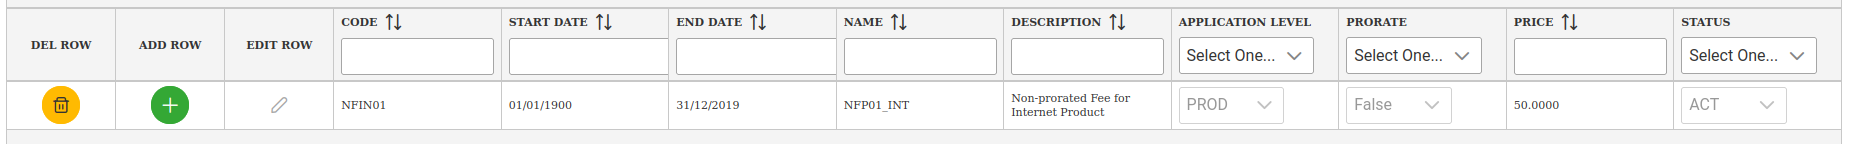
\includegraphics[width=\textwidth]{imaxes/listado-historico-tipo-consumo-tras-borrar.png}
  \caption{Listado de registros de histórico tras el borrado de un registro de histórico}
  \label{fig:listado-historico-tipo-consumo-tras-borrar}
\end{figure}




\paragraph{Editar un registro de histórico:} para ello seleccionamos el registro de histórico a editar y pulsamos el botón de edición de la columna \emph{EDIT ROW}. El registro del diálogo muestra los campos susceptibles de modificarse como editables, pudiendo realizar las modificaciones oportunas en el registro del listado. En caso de modificar el campo \emph{STATUS} del registro a \emph{CANCEL} se mostrará un cuadro de diálogo solicitando confirmación de extender este estado a todos los registros de histórico posteriores al actual, ya que se considera que una vez cancelado un registro todos los registros posteriores deben compartir dicho estado.

Supongamos el siguiente ejemplo que se ve en la \figurename~\ref{fig:listado-tipos-cuotas-inicial}: un tipo de consumo con varios registros de histórico, al que vamos a cambiar el estado del segundo registro de histórico a \emph{CANCEL}.

\begin{figure}[H]
  \centering
  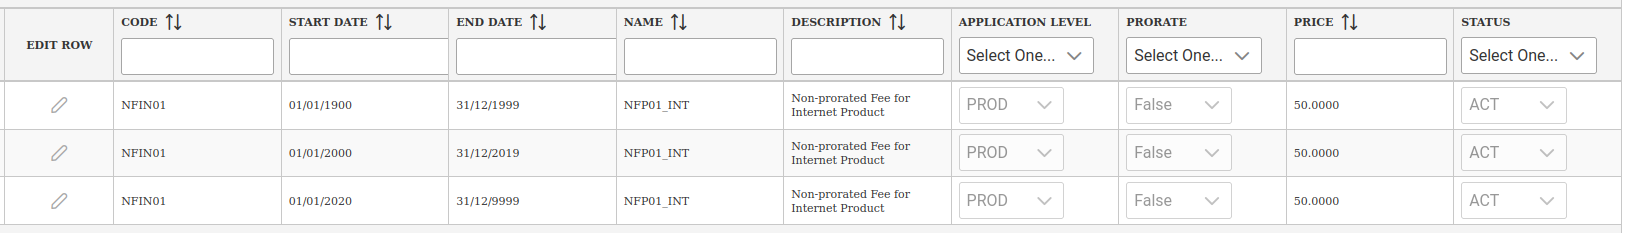
\includegraphics[width=\textwidth]{imaxes/listado-tipos-cuotas-inicial.png}
  \caption{Listado inicial de registros de histórico}
  \label{fig:listado-tipos-cuotas-inicial}
\end{figure}


Al seleccionar el estado \emph{CANCEL} del desplegable del campo correspondiente al estaod del registro se nos muestra el diálogo de confirmación de la \figurename~\ref{fig:confirmación-cambio-estado-cancelado}:

\begin{figure}[H]
  \centering
  \includegraphics[width=0.9\textwidth]{imaxes/confirmación-cambio-estado-cancelado.png}
  \caption{Diálogo de confirmación para el cambio de estado del registro de la entidad}
  \label{fig:confirmación-cambio-estado-cancelado}
\end{figure}


Pulsamos el botón \emph{OK} de confirmación de la operación y se nos muestra el listado de los registros de histórico con los estados cambiados. Pulsando el botón de confirmar la edición se confirman los cambios realizados, actualizándose el listado de los registros de histórico con los cambios producidos, incluido el cambio de estado para el registro modificado y los siguientes, tal y como se muestra en la \figurename~\ref{fig:cambio-estado-cancelado}:

\begin{figure}[H]
  \centering
  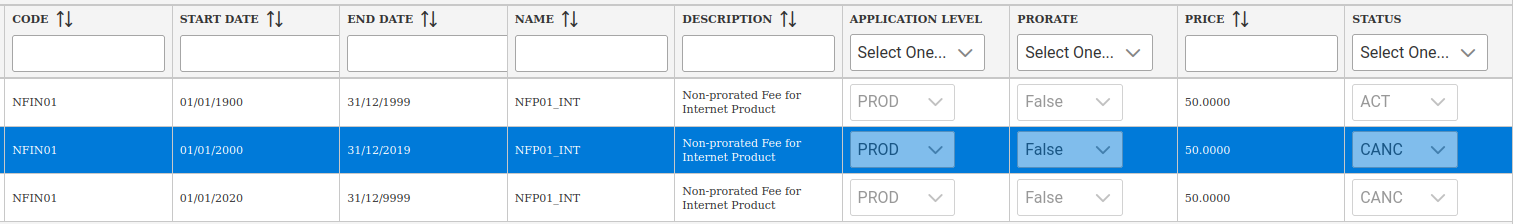
\includegraphics[width=\textwidth]{imaxes/cambio-estado-cancelado.png}
  \caption{Listado actualizado con el cambio de estado}
  \label{fig:cambio-estado-cancelado}
\end{figure}




\subsubsection{Product Type - tipo de producto}
\label{sub:product-type}

Nota: Para acceder a la pantalla que da acceso a la operativa de este tipo de entidad se desplegará la sección \emph{CATALOG} del menú principal y se seleccionará el tipo de entidad \emph{Product Type} $\rightarrow$ \emph{Product Type Definition}.

Consideramos los tipos de productos como entidades pertenecientes al catálogo de servicios propiamente dicho.

Entendemos por tipo de producto un paquete a ofertar a los clientes que tiene asociado un conjunto de tipos de cuotas y tipos de descuentos sobre esos tipos cuotas y que contiene los distintos servicios ofertados con sus correspondientes tipos de elementos facturables y tipos de promoción.

La definición completa de un tipo de producto viene dado por sí mismo y las relaciones que establece con el resto de entidades del catálogo de servicios ofertados: tipos de cuotas que aplican sobre el producto, tipos de promociones que pueden aplicar descuentos sobre esos tipos de cuotas y tipos de servicio que dependen del tipo de producto. En este apartado nos centraremos en la definición del tipo de producto \textit{per se} dejando la definición del tipo de producto con el resto de tipos de entidades para más adelante, una vez visto el resto de elementos que conforman el catálogo de servicios.

Un tipo de producto viene definido por los elementos indicados en la \tablename~\ref{tab:tipo-producto}:



\begin{table}[H]
  \centering
  \rowcolors{2}{white}{udcgray!25}
  \setlength{\leftmargini}{0.4cm}
  \resizebox{14cm}{!} {
  \begin{tabular}{|m{3cm} m{11cm}|}
  \rowcolor{udcpink!25}
  \hline
  	\textbf{Elemento} & \textbf{Descripción} \\\hline
	\textbf{CODE} & Código identificativo del tipo de producto. Es único.   \\
	\textbf{NAME} & Nombre del tipo de producto. \\
	\textbf{DESCRIPTION} & Descripción del tipo de producto. \\		
	\textbf{STATUS} & Estado del tipo del producto.
	\\\hline
  \end{tabular}
  } % end /resizebox
  \caption{Datos que definen un tipo de producto.}
  \label{tab:tipo-producto}
\end{table}

Las operaciones definidas para esta entidad son las siguientes (nota: sólo están habilitadas para usuarios con permisos de edición):
\begin{description}
\item[\underline{\textsl{\textbf{Crear nuevo tipo de producto}}}] Para crear un nuevo tipo de producto se pulsará el botón \textit{New Data} situado en la parte superior de la tabla. Aparecerá una ventana emergente que mostrará un formulario con los campos a cubrir.

\item[\underline{\textsl{\textbf{Editar tipo de producto existente}}}] Para editar un tipo de producto existente se seleccionará del listado y se pulsará el botón editar de la columna \textit{EDIT ROW} correspondiente. Se editarán los campos pertinentes directamente en la tabla para realizar las modificaciones oportunas. 

\item[\underline{\textsl{\textbf{Borrar tipo de consumo}}}] Para borrar un tipo de producto se seleccionará del listado y se pulsará el botón amarillo de borrar de la columna \textit{DEL ROW} correspondiente.
\end{description}

Todos los valores mostrados para la entidad son obligatorios y deberán cubrirse al realizar un alta o modificación. Asimismo el valor del campo CODE es único. No pueden existir dos entidades del mismo tipo con el mismo código.




\subsubsection{Service Type - tipo de servicio}
\label{sub:service-type}

Nota: Para acceder a la pantalla que da acceso a la operativa de este tipo de entidad se desplegará la sección \emph{CATALOG} del menú principal y se seleccionará el tipo de entidad \emph{Service Type} $\rightarrow$  \emph{Service Type Definition}.

Consideramos los tipos de servicios como entidades pertenecientes al catálogo de servicios propiamente dicho.

Entendemos por tipo de servicio el bien inmateriar que se le presta al cliente y que es el verdadero objetivo de la contratación.

La definición completa de un tipo de servicio viene dado por sí mismo y las relaciones que establece con el resto de entidades del catálogo de servicios ofertados: tipos de productos en los que está englobado, tipos de cuotas que pueden aplicar sobre él y los tipos de promociones que pueden aplicar descuentos sobre los distintos tipos de elementos facturables asociados al tipo de servicio. En este apartado nos centraremos en la definición del tipo de servicio \textit{per se} dejando la definición del tipo de servicio con el resto de tipos de entidades para más adelante, una vez visto el resto de elementos que conforman el catálogo de servicios.

Un tipo de servicio viene definido por los elementos indicados en la \tablename~\ref{tab:tipo-servicio}:



\begin{table}[H]
  \centering
  \rowcolors{2}{white}{udcgray!25}
  \setlength{\leftmargini}{0.4cm}
  \resizebox{14cm}{!} {
  \begin{tabular}{|m{3cm} m{11cm}|}
  \rowcolor{udcpink!25}
  \hline
  	\textbf{Elemento} & \textbf{Descripción} \\\hline
	\textbf{CODE} & Código identificativo del tipo de servicio. Es único.   \\
	\textbf{NAME} & Nombre del tipo de servicio. \\
	\textbf{DESCRIPTION} & Descripción del tipo de servicio. \\		
	\textbf{STATUS} & Estado del tipo del servicio.
	\\\hline
  \end{tabular}
  } % end /resizebox
  \caption{Datos que define un tipo de servicio.}
  \label{tab:tipo-servicio}
\end{table}

Las operaciones definidas para esta entidad son las siguientes (nota: sólo están habilitadas para usuarios con permisos de edición):
\begin{description}
\item[\underline{\textsl{\textbf{Crear nuevo tipo de producto}}}] Para crear un nuevo tipo de producto se pulsará el botón \textit{New Data} situado en la parte superior de la tabla. Aparecerá una ventana emergente que mostrará un formulario con los campos a cubrir.

\item[\underline{\textsl{\textbf{Editar tipo de producto existente}}}] Para editar un tipo de producto existente se seleccionará del listado y se pulsará el botón editar de la columna \textit{EDIT ROW} correspondiente. Se editarán los campos pertinentes directamente en la tabla para realizar las modificaciones oportunas. 

\item[\underline{\textsl{\textbf{Borrar tipo de consumo}}}] Para borrar un tipo de producto se seleccionará del listado y se pulsará el botón amarillo de borrar de la columna \textit{DEL ROW} correspondiente.
\end{description}

Todos los valores mostrados para la entidad son obligatorios y deberán cubrirse al realizar un alta o modificación. Asimismo el valor del campo CODE es único. No pueden existir dos entidades del mismo tipo con el mismo código.



\subsubsection{Promotion Type - tipo de Promoción}
\label{sub:promotion-type}

Nota: Para acceder a la pantalla que da acceso a la operativa de este tipo de entidad se desplegará la sección \emph{CATALOG} del menú principal y se seleccionará el tipo de entidad \emph{Promotion Type} $\rightarrow$  \emph{Promotion Type Definition}.

Consideramos los tipos de promociones como entidades pertenecientes al catálogo de servicios propiamente dicho.

Entendemos por tipo de promoción aquellos descuentos que pueden aplicarse sobre tipos de elementos facturables.

La definición completa de un tipo de promoción viene dado por sí mismo y las relaciones que establece con el resto de entidades del catálogo de servicios ofertados: los distintos tipos de elementos facturables sobre los que puede aplicar un descuento y las entidades facturables sobre las que aplican dichos elementos facturables.  En este apartado nos centraremos en la definición del tipo de promoción \textit{per se} dejando la definición del tipo de promoción con el resto de tipos de entidades para más adelante.

Al igual que ocurre con los tipos de cuota, los tipos de promoción pueden variar con el tiempo, modificándose las condiciones de descuento. Por lo tanto se ha considerado la necesidad de llevar un registro de estos cambios a lo largo de la vida útil de este tipo de elementos. Así pues una entidad de este tipo estará conformada por uno o varios registros con una fecha incio y una fecha fin que definen el período en el que aplican las condiciones definidas para esa entidad. Estos registros deben ser consecutivos de forma que si existen varios registros la fecha de inicio de un registro debe ser la fecha de fin del registro anterior mas un día (salvo para el primer registro que conforma el período del ciclo de vida del elemento). De igual forma la fecha de finalización de un registro debe ser la fecha de inicio del registro siguiente menos un día (salvo para el último registro que conforma el período del ciclo de vida del elemento).


Un tipo de promoción viene definido por los elementos indicados en la \tablename~\ref{tab:tipo-promoción}.
Las operaciones definidas para esta entidad son las siguientes:

\begin{table}
  \centering
  \rowcolors{2}{white}{udcgray!25}
  \setlength{\leftmargini}{0.4cm}
  \resizebox{14cm}{!} {
  \begin{tabular}{|m{4cm} m{11cm}|}
  \rowcolor{udcpink!25}
  \hline
  	\textbf{Elemento} & \textbf{Descripción} \\\hline
  	\textbf{START DATE} & Fecha de inicio del período temporal para el que aplican las condiciones especificadas para dicho período.\\
  	\textbf{END DATE} & Fecha de finalización del período temporal para el que aplican las condiciones especificadas para dicho período.\\
  	\textbf{CODE} & Código identificativo del tipo de promoción. Es único.\\
	\textbf{NAME} & Nombre del tipo de promoción.\\
	\textbf{DESCRIPTION} & Descripción del tipo de promoción.\\
	\textbf{APPLICATION LEVEL} & Nivel de aplicación del tipo de promoción, esto es, a qué entidad facturable va asociado. Los niveles de aplicación están definidos en la correspondiente entidad de \emph{PARAMETERS} definida en la sección \ref{sub:parametrizacion}.\\	
	\textbf{DISCOUNT TYPE} & Indica el tipo de descuento a aplicar por el tipo de promoción. Los distintos tipos de descuento definidos en la correspondiente entidad de \emph{PARAMETERS} definida en la sección \ref{sub:parametrizacion}..\\
	\textbf{DISCOUNT VALUE} & Descuento a aplicar en función del tipo de descuento definido en el tipo de promoción (volumen, unidades, porcentaje\dots.\\
	\textbf{STATUS} & Estado del tipo de promoción.	
	\\\hline
  \end{tabular}
  } % end /resizebox
  \caption{Datos que define un tipo de promoción.}
  \label{tab:tipo-promoción}
\end{table}

\begin{description}
\item[\underline{\textsl{\textbf{Buscar un tipo de promoción existente}}}] Esta operación está disponible para todos los usuarios de la aplicación.
Puesto que los tipos de promoción son entidades con histórico, por motivos de operatividad no se muestra el listado de todas las entidades del sistema por defecto, si no que se establecen unos criterios de búsqueda para seleccionar el tipo de promoción a consultar. Para ello se define un área de búsqueda en los que se definen los criterios de búsqueda a tener en cuenta:
\begin{itemize}
\item Buscar todos los históricos de los tipos de consumo. Se realizará una búsqueda de todos los históricos de los distintos tipos de consumo.
\item Buscar por fecha. Se realizará una búsqueda de los históricos de todos los tipos de consumo existentes en el sistema para los que la fecha de búsqueda definida se encuentre entre la fecha de inicio y fin del registro de histórico. Opción marcada por defecto
\end{itemize}

Pulsando el botón \emph{Search} se mostrará un panel emergente con el listado de los registros encontrados. Seleccionaremos el elemento sobre el que queramos operar pulsando el botón amarillo de la columna \emph{Show Historic} y se mostrará el área de históricos de la entidad con los distintos registros de histórico existentes de forma análogo a lo ya visto en la sección \ref{sub:fee-type}

\item[\underline{\textsl{\textbf{Crear nuevo tipo de promoción}}}] Esta operación sólo está diponible para usuarios con permisos de edición.
Para crear un nuevo consumo se pulsará el botón \textit{New Data} situado en la parte superior de la tabla. Aparecerá una ventana emergente que mostrará un formulario con los campos a cubrir. Por defecto se establecen como fecha de inicio y fin del nuevo tipo de cuota las fechas 01/01/1900 y 31/12/9999.

\item[\underline{\textsl{\textbf{Editar registro de histórico de un tipo de promoción existente}}}] Esta operación sólo está diponible para usuarios con permisos de edición.
Para editar un tipo de consumo existente se seleccionará del listado y se pulsará el botón editar de la columna \textit{EDIT ROW} correspondiente. Se editarán los campos pertinentes directamente en la tabla para realizar las modificaciones oportunas teniendo en cuenta los criterios de fechas establecidos (definidos en la sección \ref{sub:histórico-conceptos} de la página \pageref{sub:histórico-conceptos}).

\item[\underline{\textsl{\textbf{Añadir registro de histórico de un tipo de promoción existente}}}] Esta operación sólo está diponible para usuarios con permisos de edición.
Para añadir un nuevo registro de histórico sobre tipo de consumo existente se seleccionará del listado el registro en el que se ubicará el nuevo registro a añadir 
y se pulsará el botón añadir de la columna \textit{ADD ROW} correspondiente. Aparecerá una nueva ventana emergente como la que se muestra en la operación de creación, pero con los campos cubiertos con la información del registro sobre el que se va a añadir el nuevo registro y se realizán las moficaciones oportunas teniendo en cuenta los criterios de fechas establecidos (definidos en la sección \ref{sub:histórico-conceptos} de la página \pageref{sub:histórico-conceptos}).

\item[\underline{\textsl{\textbf{Borrar registro de histórico del tipo de promoción}}}] Esta operación sólo está diponible para usuarios con permisos de edición.
Para borrar un registro de histórico del tipo de consumo se seleccionará del listado el registro a borrar y se pulsará el botón amarillo de borrar de la columna \textit{DEL ROW} correspondiente.

\item[\underline{\textsl{\textbf{Borrar el tipo de promoción}}}] Esta operación sólo está diponible para usuarios con permisos de edición.
Para borrar completamente un tipo de cuota se deben borrar uno a uno todos los registros de histórico del tipo de cuota según lo indicado en el punto anterior.
\end{description}

Todos los valores mostrados para la entidad son obligatorios y deberán cubrirse al realizar un alta o modificación. Asimismo el valor del campo CODE es único. No pueden existir dos entidades del mismo tipo con el mismo código.

La realización de las distintas operaciones es análogo a lo visto para las operaciones de los tipos de cuotas. Para más información consulte la sección \ref{sub:fee-type}.


\subsubsection{Product Fee Type - Relación entre tipo de Producto y de Cuota}
\label{sub:product-fee-type-relation}

Nota: Para acceder a la pantalla que da acceso a la operativa de este tipo de entidad se desplegará la sección \emph{CATALOG} del menú principal y se seleccionará el tipo de entidad \emph{Product Type} $\rightarrow$  \emph{Product Fee Type}.


A continuación veremos cómo gestionar las distintas relaciones que se establecen entre un tipo de producto y los tipos de cuotas que pueden asociarse al tipo de producto dado.


En la parte superior de la pantalla se encuentra el área de búsqueda. Pulsando el botón verde \emph{SEARCH} aparece un listado de todos los productos del sistema. Seleccionaremos el tipo de producto sobre el que queramos consultar las relaciones de las entiades pulsando el botón amarillo de la columna \emph{Show Data}. A continuación se visualizará el área de relaciones del producto en los que se muestran los tipos de cuotas para los que existe una relación con el producto (ver \figurename~\ref{fig:area-relacion-tipos-entidades}).


\begin{figure}[H]
  \centering
  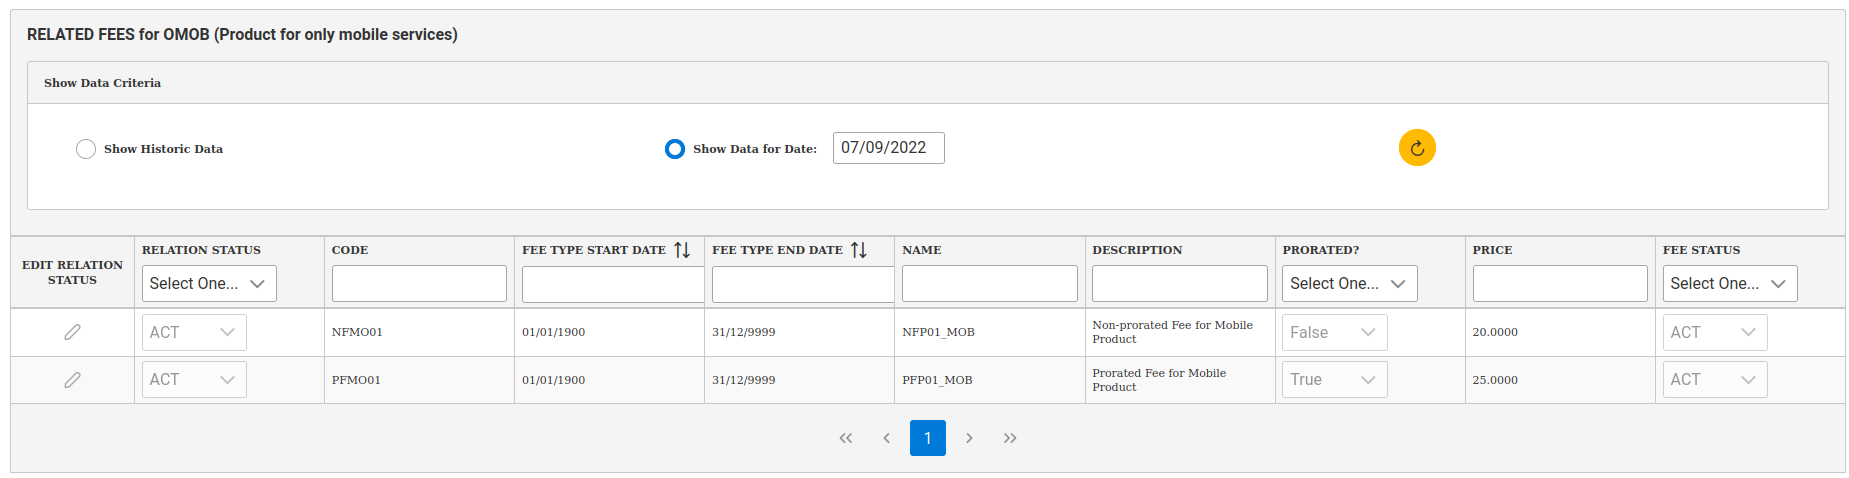
\includegraphics[width=\textwidth]{imaxes/area-relacion-tipos-entidades.png}
  \caption{Área que muestra los tipos de entidad cuota relacionada con el producto}
  \label{fig:area-relacion-tipos-entidades}
\end{figure}



Al ser el tipo de cuota una entidad con registro de histórico en el área de relaciones se muestran por defecto los registros para los que la fecha definida en el área de visualización de la entidad relacionada (que por defecto es la fecha actual) se encuentra comprendida en el período del histórico. Si queremos mostrar todos los registros de histórico de las distintas entidades relacionadas seleccionaremos la opción de \emph{Show Historic Data} y pulsaremos el botón de refrescar que se encuentra a la derecha del área de criterios de visualización. Lo mismo si queremos que se muestren los históricos para otra fecha distinta de la especificada por defecto: bastará con modificar la fecha y pulsar el botón de refrescar.

Si accedemos a la vista con un usuario con permisos de edición se mostrará otro listado con los tipos de cuota con nivel de aplicación producto para los que no se ha establecido relación con el tipo de producto consultado, así como dos botones, uno con una flecha apuntando hacia arriba y otro con una flecha apuntando hacia abajo. Estos botones permitirán añadir un tipo de cuota a la relación con el producto o eliminar dicha relación respectivamente. 



\begin{figure}[H]
  \centering
  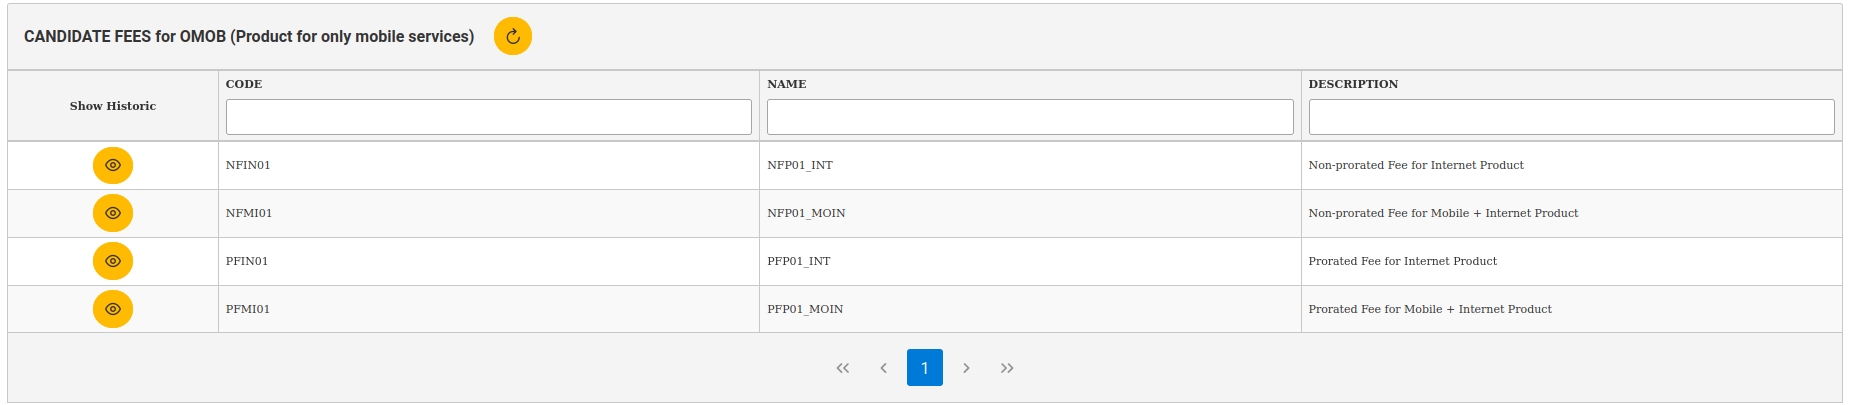
\includegraphics[width=\textwidth]{imaxes/area-tipos-entidades-candidatas.png}
  \caption{Área que muestra los tipos de entidad cuota candidatas a establecer relación con el producto}
  \label{fig:area-tipos-entidades-candidatas}
\end{figure}



\begin{figure}[H]
  \centering
  \includegraphics[width=0.15\textwidth]{imaxes/botones-añadir-eliminar-relacion-tipos.png}
  \caption{Detalle de los botones para gestionar las relaciones: a la izquierda el botón de añadir relación, a la derecha el botón de eliminar relación}
  \label{fig:botones-añadir-eliminar-relacion-tipos}
\end{figure}

A mayores el listado de entidades relacionadas permite editar el estado de la relación mientras que en el listado de candidatos existe un botón que permite ver el histórico de la entidad candidata, siempre que el usuario tenga permisos de edición.



Las operaciones definidas para esta vista son las siguientes (nota: sólo están habilitadas para usuarios con permisos de edición):
\begin{description}
\item[\underline{\textsl{\textbf{Añadir una nueva entidad tipo cuota a la relación}}}] Para añadir una nueva relación seleccionaremos el tipo de cuota deseado del listado de candidatos y pulsaremos el botón de la flecha que apunta hacia arriba (hacia el listado de entidades relacionadas). Se eliminará el registro del listado de candidatos y se añadirá al listado de tipos de cuotas relacionadas.

\item[\underline{\textsl{\textbf{Eliminar una entidad tipo cuota existente de la relación}}}] Para eliminar una relación existente seleccionaremos el tipo de cuota deseado del listado de relaciones y pulsaremos el botón de la flecha que apunta hacia abajo (hacia el listado de entidades candidatas). Se eliminará el registro del listado de relaciones y se añadirá al listado de tipos de cuotas candidatas.

\item[\underline{\textsl{\textbf{Editar el estado de la relación de histórico de un tipo de cuota existente}}}] Para editar el estado de la relación se seleccionará la entidad del tipo cuota deseada del listado de entidades relacionadas y se pulsará el botón editar de la columna \textit{EDIT RELATION STATUS} correspondiente. Se editará el campo \emph{RELATION STATUS}  pertinentes directamente en la tabla para realizar las modificaciones oportunas.

\item[\underline{\textsl{\textbf{Visualizar el registro de históricos de un tipo de cuota candidata}}}] Para visualizar todos los históricos de un tipo de cuota candidata se seleccionará la entidad del tipo cuota deseada del listado de entidades relacionadas y se pulsará el botón amarillo de la columna \textit{SHOW HISTORICS}. Se mostrará un panel que muestra el listado de históricos para la entidad seleccionada.
\end{description}


\subsubsection{Product Service Type - Relación entre tipo de Producto y de Servicio}
\label{sub:product-service-type-relation}

Nota: Para acceder a la pantalla que da acceso a la operativa de este tipo de entidad se desplegará la sección \emph{CATALOG} del menú principal y se seleccionará el tipo de entidad \emph{Product Type} $\rightarrow$  \emph{Promotion Service Type}.


A continuación veremos cómo gestionar las distintas relaciones que se establecen entre un tipo de producto y los tipos de servicio que pueden contener.


En la parte superior de la pantalla se encuentra el área de búsqueda. Pulsando el botón verde \emph{SEARCH} aparece un listado de todos los productos del sistema. Seleccionaremos el tipo de producto sobre el que queramos consultar las relaciones de las entiades pulsando el botón amarillo de la columna \emph{Show Data}. A continuación se visualizará el área de relaciones del producto en los que se muestran los tipos de servicio para los que existe una relación con el producto.

Si accedemos a la vista con un usuario con permisos de edición se mostrará otro listado con los tipos de servicio para los que no se ha establecido relación con el tipo de producto consultado, así como dos botones, uno con una flecha apuntando hacia arriba y otro con una flecha apuntando hacia abajo. Estos botones permitirán añadir un tipo de servicio a la relación con el producto o eliminar dicha relación respectivamente. 

A mayores el listado de entidades relacionadas permite editar el estado de la relación mientras que en el listado de candidatos existe un botón que permite ver el histórico de la entidad candidata, siempre que el usuario tenga permisos de edición.


Las operaciones definidas para esta vista son las siguientes (nota: sólo están habilitadas para usuarios con permisos de edición):
\begin{description}
\item[\underline{\textsl{\textbf{Añadir una nueva entidad tipo servicio a la relación}}}] Para añadir una nueva relación seleccionaremos el tipo de servicio deseado del listado de candidatos y pulsaremos el botón de la flecha que apunta hacia arriba (hacia el listado de entidades relacionadas). Se eliminará el registro del listado de candidatos y se añadirá al listado de tipos de servicio relacionados.

\item[\underline{\textsl{\textbf{Eliminar una entidad tipo servicio existente de la relación}}}] Para eliminar una relación existente seleccionaremos el tipo de servicio deseado del listado de relaciones y pulsaremos el botón de la flecha que apunta hacia abajo (hacia el listado de entidades candidatas). Se eliminará el registro del listado de relaciones y se añadirá al listado de tipos de servicios candidatas.

\item[\underline{\textsl{\textbf{Editar el estado de la relación de histórico de un tipo de servicio existente}}}] Para editar el estado de la relación se seleccionará la entidad del tipo servicio de consumo deseado del listado de entidades relacionadas y se pulsará el botón editar de la columna \textit{EDIT RELATION STATUS} correspondiente. Se editará el campo \emph{RELATION STATUS} pertinentes directamente en la tabla para realizar las modificaciones oportunas.
\end{description}



\subsubsection{Product Promotion Type - Relación entre tipo de Producto y de Promoción}
\label{sub:product-promotion-type-relation}

Nota: Para acceder a la pantalla que da acceso a la operativa de este tipo de entidad se desplegará la sección \emph{CATALOG} del menú principal y se seleccionará el tipo de entidad \emph{Product Type} $\rightarrow$  \emph{Product Promotion Type}.


A continuación veremos cómo gestionar las distintas relaciones que se establecen entre un tipo de producto y los tipos de promociones que pueden asociarse al tipo de producto dado.


En la parte superior de la pantalla se encuentra el área de búsqueda. Pulsando el botón verde \emph{SEARCH} aparece un listado de todos los productos del sistema. Seleccionaremos el tipo de producto sobre el que queramos consultar las relaciones de las entiades pulsando el botón amarillo de la columna \emph{Show Data}. A continuación se visualizará el área de relaciones del producto en los que se muestran los tipos de promociones para los que existe una relación con el producto.

Al ser el tipo de promoción una entidad con registro de histórico en el área de relaciones se muestran por defecto los registros para los que la fecha definida en el área de visualización de la entidad relacionada (que por defecto es la fecha actual) se encuentra comprendida en el período del histórico. Si queremos mostrar todos los registros de histórico de las distintas entidades relacionadas seleccionaremos la opción de Show Historic Data y pulsaremos el botón de refrescar que se encuentra a la derecha del área de criterios de visualización. Lo mismo si queremos que se muestren los históricos para otra fecha distinta de la especificada por defecto: bastará con modificar la fecha y pulsar el botón de refrescar.

Si accedemos a la vista con un usuario con permisos de edición se mostrará otro listado con los tipos de promoción con nivel de aplicación producto para los que no se ha establecido relación con el tipo de producto consultado, así como dos botones, uno con una flecha apuntando hacia arriba y otro con una flecha apuntando hacia abajo. Estos botones permitirán añadir un tipo de promoción a la relación con el producto o eliminar dicha relación respectivamente. 

A mayores el listado de entidades relacionadas permite editar el estado de la relación mientras que en el listado de candidatos existe un botón que permite ver el histórico de la entidad candidata, siempre que el usuario cuente con permisos de edición.


Las operaciones definidas para esta vista son las siguientes (nota: sólo están habilitadas para usuarios con permisos de edición):
\begin{description}
\item[\underline{\textsl{\textbf{Añadir una nueva entidad tipo promoción a la relación}}}] Para añadir una nueva relación seleccionaremos el tipo de promoción deseado del listado de candidatos y pulsaremos el botón de la flecha que apunta hacia arriba (hacia el listado de entidades relacionadas). Se eliminará el registro del listado de candidatos y se añadirá al listado de tipos de cuotas relacionadas.

\item[\underline{\textsl{\textbf{Eliminar una entidad tipo promoción existente de la relación}}}] Para eliminar una relación existente seleccionaremos el tipo de promoción deseado del listado de relaciones y pulsaremos el botón de la flecha que apunta hacia abajo (hacia el listado de entidades candidatas). Se eliminará el registro del listado de relaciones y se añadirá al listado de tipos de promociones candidatas.

\item[\underline{\textsl{\textbf{Editar el estado de la relación de histórico de un tipo de promoción existente}}}] Para editar el estado de la relación se seleccionará la entidad del tipo promoción  deseada del listado de entidades relacionadas y se pulsará el botón editar de la columna \textit{EDIT RELATION STATUS} correspondiente. Se editará el campo \emph{RELATION STATUS}  pertinentes directamente en la tabla para realizar las modificaciones oportunas.

\item[\underline{\textsl{\textbf{Visualizar el registro de históricos de un tipo de promoción candidata}}}] Para visualizar todos los históricos de un tipo de promoción candidata se seleccionará la entidad del tipo promoción deseada del listado de entidades relacionadas y se pulsará el botón amarillo de la columna \textit{SHOW HISTORICS}. Se mostrará un panel que muestra el listado de históricos para la entidad seleccionada. 
\end{description}


\subsubsection{Service Fee Type - Relación entre tipo de Servicio y de Cuota}
\label{sub:product-fee-type-relation}

Nota: Para acceder a la pantalla que da acceso a la operativa de este tipo de entidad se desplegará la sección \emph{CATALOG} del menú principal y se seleccionará el tipo de entidad \emph{Service Type} $\rightarrow$  \emph{Service Fee Type}.


A continuación veremos cómo gestionar las distintas relaciones que se establecen entre un tipo de servicio y los tipos de cuotas que pueden asociarse al tipo de servicio dado.


En la parte superior de la pantalla se encuentra el área de búsqueda. Pulsando el botón verde \emph{SEARCH} aparece un listado de todos los servicios del sistema. Seleccionaremos el tipo de servicio sobre el que queramos consultar las relaciones de las entiades pulsando el botón amarillo de la columna \emph{Show Data}. A continuación se visualizará el área de relaciones del producto en los que se muestran los tipos de cuotas para los que existe una relación con el servicio.

Al ser el tipo de cuota una entidad con registro de histórico en el área de relaciones se muestran por defecto los registros para los que la fecha definida en el área de visualización de la entidad relacionada (que por defecto es la fecha actual) se encuentra comprendida en el período del histórico. Si queremos mostrar todos los registros de histórico de las distintas entidades relacionadas seleccionaremos la opción de Show Historic Data y pulsaremos el botón de refrescar que se encuentra a la derecha del área de criterios de visualización. Lo mismo si queremos que se muestren los históricos para otra fecha distinta de la especificada por defecto: bastará con modificar la fecha y pulsar el botón de refrescar.

Si accedemos a la vista con un usuario con permisos de edición se mostrará otro listado con los tipos de cuota con nivel de aplicación servicio para los que no se ha establecido relación con el tipo de servicio consultado, así como dos botones, uno con una flecha apuntando hacia arriba y otro con una flecha apuntando hacia abajo. Estos botones permitirán añadir un tipo de cuota a la relación con el servicio o eliminar dicha relación respectivamente. 

A mayores el listado de entidades relacionadas permite editar el estado de la relación mientras que en el listado de candidatos existe un botón que permite ver el histórico de la entidad candidata, siempre que el usuario cuente con permisos de edición.



Las operaciones definidas para esta vista son las siguientes (nota: sólo están habilitadas para usuarios con permisos de edición):
\begin{description}
\item[\underline{\textsl{\textbf{Añadir una nueva entidad tipo cuota a la relación}}}] Para añadir una nueva relación seleccionaremos el tipo de cuota deseado del listado de candidatos y pulsaremos el botón de la flecha que apunta hacia arriba (hacia el listado de entidades relacionadas). Se eliminará el registro del listado de candidatos y se añadirá al listado de tipos de cuotas relacionadas.

\item[\underline{\textsl{\textbf{Eliminar una entidad tipo cuota existente de la relación}}}] Para eliminar una relación existente seleccionaremos el tipo de cuota deseado del listado de relaciones y pulsaremos el botón de la flecha que apunta hacia abajo (hacia el listado de entidades candidatas). Se eliminará el registro del listado de relaciones y se añadirá al listado de tipos de cuotas candidatas.

\item[\underline{\textsl{\textbf{Editar el estado de la relación de histórico de un tipo de cuota existente}}}] Para editar el estado de la relación se seleccionará la entidad del tipo cuota deseada del listado de entidades relacionadas y se pulsará el botón editar de la columna \textit{EDIT RELATION STATUS} correspondiente. Se editará el campo \emph{RELATION STATUS}  pertinentes directamente en la tabla para realizar las modificaciones oportunas.

\item[\underline{\textsl{\textbf{Visualizar el registro de históricos de un tipo de cuota candidata}}}] Para visualizar todos los históricos de un tipo de cuota candidata se seleccionará la entidad del tipo cuota deseada del listado de entidades relacionadas y se pulsará el botón amarillo de la columna \textit{SHOW HISTORICS}. Se mostrará un panel que muestra el listado de históricos para la entidad seleccionada.
\end{description}



\subsubsection{Service Promotion Type - Relación entre tipo de Servicio y de Promoción}
\label{sub:product-promotion-type-relation}

Nota: Para acceder a la pantalla que da acceso a la operativa de este tipo de entidad se desplegará la sección \emph{CATALOG} del menú principal y se seleccionará el tipo de entidad \emph{Service Type} $\rightarrow$  \emph{Service Promotion Type}.


A continuación veremos cómo gestionar las distintas relaciones que se establecen entre un tipo de servicio y los tipos de promociones que pueden asociarse al tipo de servicio dado.


En la parte superior de la pantalla se encuentra el área de búsqueda. Pulsando el botón verde \emph{SEARCH} aparece un listado de todos los servicios del sistema. Seleccionaremos el tipo de producto sobre el que queramos consultar las relaciones de las entiades pulsando el botón amarillo de la columna \emph{Show Data}. A continuación se visualizará el área de relaciones del servicio en los que se muestran los tipos de promoción para los que existe una relación con el servicio.

Al ser el tipo de promoción una entidad con registro de histórico en el área de relaciones se muestran por defecto los registros para los que la fecha definida en el área de visualización de la entidad relacionada (que por defecto es la fecha actual) se encuentra comprendida en el período del histórico. Si queremos mostrar todos los registros de histórico de las distintas entidades relacionadas seleccionaremos la opción de Show Historic Data y pulsaremos el botón de refrescar que se encuentra a la derecha del área de criterios de visualización. Lo mismo si queremos que se muestren los históricos para otra fecha distinta de la especificada por defecto: bastará con modificar la fecha y pulsar el botón de refrescar.

Si accedemos a la vista con un usuario con permisos de edición se mostrará otro listado con los tipos de promoción con nivel de aplicación servicio para los que no se ha establecido relación con el tipo de servicio consultado, así como dos botones, uno con una flecha apuntando hacia arriba y otro con una flecha apuntando hacia abajo. Estos botones permitirán añadir un tipo de promoción a la relación con el servicio o eliminar dicha relación respectivamente. 

A mayores el listado de entidades relacionadas permite editar el estado de la relación mientras que en el listado de candidatos existe un botón que permite ver el histórico de la entidad candidata, siempre que el usuario cuente con permisos de edición


Las operaciones definidas para esta vista son las siguientes (nota: sólo están habilitadas para usuarios con permisos de edición):
\begin{description}
\item[\underline{\textsl{\textbf{Añadir una nueva entidad tipo promoción a la relación}}}] Para añadir una nueva relación seleccionaremos el tipo de promoción deseado del listado de candidatos y pulsaremos el botón de la flecha que apunta hacia arriba (hacia el listado de entidades relacionadas). Se eliminará el registro del listado de candidatos y se añadirá al listado de tipos de cuotas relacionadas.

\item[\underline{\textsl{\textbf{Eliminar una entidad tipo promoción existente de la relación}}}] Para eliminar una relación existente seleccionaremos el tipo de promoción deseado del listado de relaciones y pulsaremos el botón de la flecha que apunta hacia abajo (hacia el listado de entidades candidatas). Se eliminará el registro del listado de relaciones y se añadirá al listado de tipos de promociones candidatas.

\item[\underline{\textsl{\textbf{Editar el estado de la relación de histórico de un tipo de promoción existente}}}] Para editar el estado de la relación se seleccionará la entidad del tipo promoción  deseada del listado de entidades relacionadas y se pulsará el botón editar de la columna \textit{EDIT RELATION STATUS} correspondiente. Se editará el campo \emph{RELATION STATUS}  pertinentes directamente en la tabla para realizar las modificaciones oportunas.

\item[\underline{\textsl{\textbf{Visualizar el registro de históricos de un tipo de promoción candidata}}}]
Para visualizar todos los históricos de un tipo de promoción candidata se seleccionará la entidad del tipo promoción deseada del listado de entidades relacionadas y se pulsará el botón amarillo de la columna \textit{SHOW HISTORICS}. Se mostrará un panel que muestra el listado de históricos para la entidad seleccionada. 
\end{description}


\subsubsection{Promotion Fee Type - Relación entre tipo de Promoción y de Cuota}
\label{sub:promotion-fee-type-relation}

Nota: Para acceder a la pantalla que da acceso a la operativa de este tipo de entidad se desplegará la sección \emph{CATALOG} del menú principal y se seleccionará el tipo de entidad \emph{Promotion Type} $\rightarrow$  \emph{Promotion Fee Type Discount}.


A continuación veremos cómo gestionar las distintas relaciones que se establecen entre un tipo de promoción y los tipos de consumos que pueden asociarse al tipo de promoción dado.


En la parte superior de la pantalla se encuentra el área de búsqueda. Puesto que los tipos de promoción son entidades con histórico, dicha área contendrá los criterios de búsqueda según lo especificado en las secciones relativas a los tipos de entidad con histórico \ref{sub:fee-type} y \ref{sub:promotion-type}. 
Seleccionaremos el tipo de promoción sobre el que queramos consultar las relaciones de las entiades pulsando el botón amarillo de la columna \emph{Show Data}. A continuación se visualizará el área de relaciones de la promoción en los que se muestran los tipos de cuotas para los que existe una relación con la promoción.


Al ser el tipo de cuota una entidad con registro de histórico en el área de relaciones se muestran por defecto los registros para los que la fecha definida en el área de visualización de la entidad relacionada (que por defecto es la fecha actual) se encuentra comprendida en el período del histórico. Si queremos mostrar todos los registros de histórico de las distintas entidades relacionadas seleccionaremos la opción de Show Historic Data y pulsaremos el botón de refrescar que se encuentra a la derecha del área de criterios de visualización. Lo mismo si queremos que se muestren los históricos para otra fecha distinta de la especificada por defecto: bastará con modificar la fecha y pulsar el botón de refrescar.

Si accedemos a la vista con un usuario con permisos de edición se mostrará otro listado con los tipos de cuota con el mismo nivel de aplicación que la promoción para los que no se ha establecido relación con el tipo de promoción consultado, así como dos botones, uno con una flecha apuntando hacia arriba y otro con una flecha apuntando hacia abajo. Estos botones permitirán añadir un tipo de cuota a la relación con el promoción o eliminar dicha relación respectivamente. 

A mayores el listado de entidades relacionadas permite editar el estado de la relación mientras que en el listado de candidatos existe un botón que permite ver el histórico de la entidad candidata, siempre que el usuario disponga de permisos de edición.


Las operaciones definidas para esta vista son las siguientes (nota: sólo están habilitadas para usuarios con permisos de edición):
\begin{description}
\item[\underline{\textsl{\textbf{Añadir una nueva entidad tipo cuota a la relación}}}] Para añadir una nueva relación seleccionaremos el tipo de cuota deseado del listado de candidatos y pulsaremos el botón de la flecha que apunta hacia arriba (hacia el listado de entidades relacionadas). Se eliminará el registro del listado de candidatos y se añadirá al listado de tipos de cuotas relacionadas.

\item[\underline{\textsl{\textbf{Eliminar una entidad tipo cuota existente de la relación}}}] Para eliminar una relación existente seleccionaremos el tipo de cuota deseado del listado de relaciones y pulsaremos el botón de la flecha que apunta hacia abajo (hacia el listado de entidades candidatas). Se eliminará el registro del listado de relaciones y se añadirá al listado de tipos de promociones candidatas.

\item[\underline{\textsl{\textbf{Editar el estado de la relación de histórico de un tipo de cuota existente}}}] Para editar el estado de la relación se seleccionará la entidad del tipo cuota  deseada del listado de entidades relacionadas y se pulsará el botón editar de la columna \textit{EDIT RELATION STATUS} correspondiente. Se editará el campo \emph{RELATION STATUS} pertinente directamente en la tabla para realizar las modificaciones oportunas.

\item[\underline{\textsl{\textbf{Visualizar el registro de históricos de un tipo de cuota candidata}}}] Para visualizar todos los históricos de un tipo de cuota candidata se seleccionará la entidad del tipo cuota deseada del listado de entidades relacionadas y se pulsará el botón amarillo de la columna \textit{SHOW HISTORICS}. Se mostrará un panel que muestra el listado de históricos para la entidad seleccionada. 
\end{description}



\subsubsection{Promotion Consumption Type - Relación entre tipo de Promoción y de Consumo}
\label{sub:promotion-consumption-type-relation}

Nota: Para acceder a la pantalla que da acceso a la operativa de este tipo de entidad se desplegará la sección \emph{CATALOG} del menú principal y se seleccionará el tipo de entidad \emph{Promotion Type} $\rightarrow$  \emph{Promotion Consumption Type Discount}.


A continuación veremos cómo gestionar las distintas relaciones que se establecen entre un tipo de promoción y los tipos de consumos que pueden asociarse al tipo de promoción dado.


En la parte superior de la pantalla se encuentra el área de búsqueda. Puesto que los tipos de promoción son entidades con histórico, dicha área contendrá los criterios de búsqueda según lo especificado en las secciones relativas a los tipos de entidad con histórico \ref{sub:fee-type} y \ref{sub:promotion-type}. 
Seleccionaremos el tipo de promoción sobre el que queramos consultar las relaciones de las entiades pulsando el botón amarillo de la columna \emph{Show Data}. A continuación se visualizará el área de relaciones de la promoción en los que se muestran los tipos de consumos para los que existe una relación con la promoción.


Si accedemos a la vista con un usuario con permisos de edición se mostrará otro listado con los tipos de consumo con el mismo nivel de aplicación que la promoción para los que no se ha establecido relación con el tipo de promoción consultado, así como dos botones, uno con una flecha apuntando hacia arriba y otro con una flecha apuntando hacia abajo. Estos botones permitirán añadir un tipo de consumo a la relación con el promoción o eliminar dicha relación respectivamente. 

A mayores el listado de entidades relacionadas permite editar el estado de la relación, siempre que el usuario disponga de permisos de edición.


Las operaciones definidas para esta vista son las siguientes (nota: sólo están habilitadas para usuarios con permisos de edición):
\begin{description}
\item[\underline{\textsl{\textbf{Añadir una nueva entidad tipo consumo a la relación}}}] Para añadir una nueva relación seleccionaremos el tipo de consumo deseado del listado de candidatos y pulsaremos el botón de la flecha que apunta hacia arriba (hacia el listado de entidades relacionadas). Se eliminará el registro del listado de candidatos y se añadirá al listado de tipos de consumos relacionadas.

\item[\underline{\textsl{\textbf{Eliminar una entidad tipo consumo existente de la relación}}}] Para eliminar una relación existente seleccionaremos el tipo de consumo deseado del listado de relaciones y pulsaremos el botón de la flecha que apunta hacia abajo (hacia el listado de entidades candidatas). Se eliminará el registro del listado de relaciones y se añadirá al listado de tipos de promociones candidatas.

\item[\underline{\textsl{\textbf{Editar el estado de la relación de histórico de un tipo de consumo existente}}}] Para editar el estado de la relación se seleccionará la entidad del tipo consumo  deseada del listado de entidades relacionadas y se pulsará el botón editar de la columna \textit{EDIT RELATION STATUS} correspondiente. Se editará el campo \emph{RELATION STATUS} pertinente directamente en la tabla para realizar las modificaciones oportunas.
\end{description}



\subsection{Contratación}
\label{sub:contratacion}

Las contrataciones del sistema están formadas por la aplicación de las definiciones vistas en el catálogo al mundo real para satisfacer las necesidades de un cliente de la empresa.

Para ello se cuenta con la cartera de clientes, entidad conformada por los distintos clientes de la empresa que han contratado diferentes productos y a los que la empresa presta los servicios contratados.

Un cliente puede tener una o varias cuentas, que son las que definen el conjunto de contrataciones de los distintos productos, servicios, cuotas y promociones específicas para dicho cliente.

Puesto que los elementos de contratación pueden variar (y mucho) a lo largo de su ciclo de vida, se han definido todos ellos como elementos con histórico, por lo que aplican las restricciones relativas a los registros de histórico indicadas en secciones anteriores.

Se definen cinco estados distintos para las entidades de contratación:
\begin{description}
\item[ACTIVE] Estado activo. Para las entidades de contratación que están en vigencia.
\item[CANCEL] Estado cancelado. Para las entidades de contratación que han cursado baja.
\item[PEND] Estado pendiente. Para las entidades de contratación pendientes de finalizar su proceso de provisión. Este estado se ha definido con vistas a una interacción con un sistema de provisión a desarrollar en el futuro.
\item[SUSP] Estado suspendido. Para las entidades de contratación que actualmente tienen su estado suspendido, por ejemplo una suspensión temporal solicitada por el cliente porque durante un período de tiempo no va a usar un determinado servicio.
\item[DEB] Estado deuda. Para las entidades de contratación cuyo cliente ha recurrido en impagos.
\end{description}


Todos los usuarios del sistema tienen acceso a los elementos de contratación, pero aquellos que tengan permisos de edición (perfil ADMIN o MODIF) podrán gestionarlos (realizar altas, bajas y modificaciones). Los usuarios con el perfil READ sólo podrán acceder en modo consulta, y no se mostrarán habilitados los correspondientes botones para las operaciones de gestión. Por comodidad las imágenes que proceden a ilustrar esta sección se corresponderán con el acceso a las vistas de un usuario con permisos de edición. Los usuarios sin estos permisos verán la misma pantalla pero sin los botones que permiten la gestión de los datos.

A continuación veremos en detalle cada una de las vistas que conforman los distintos elementos de la contratación a los que se accede a través del menú  \emph{CONTRACT}. Todas las vistas están orientadas a consultar una instancia en particular, ya que el volumen de elementos contratados deberá exceder con creces el volumen de productos contratados y mostrar todos los elementos en una única vista haría inmanejable el sistema.



\subsubsection{Customer - Clientes}
\label{sub:customer}

Esta vista muestra la información relativa a los clientes contenidos en la cartera de clientes de la empresa. La \tablename~\ref{tab:cliente} recoge los elementos más relevantes en la definición de un cliente.
Las operaciones definidas para esta entidad son las siguientes:

\begin{table}
  \centering
  \rowcolors{2}{white}{udcgray!25}
  \setlength{\leftmargini}{0.4cm}
  \resizebox{14cm}{!} {
  \begin{tabular}{|m{6cm} m{8cm}|}
  \rowcolor{udcpink!25}
  \hline
  	\textbf{Elemento} & \textbf{Descripción} \\\hline
  	\textbf{START DATE} & Fecha de inicio del período temporal para el que aplican las condiciones especificadas para dicho período.\\
  	\textbf{END DATE} & Fecha de finalización del período temporal para el que aplican las condiciones especificadas para dicho período.\\
	\textbf{CLIENT TYPE} & Tipo de cliente asociado al cliente.\\
	\textbf{CLIENT ID} & Identificador unívoco del cliente generado por la apliación.\\
	\textbf{NAME} & Nombre del cliente.\\
	\textbf{1st SURNAME} & Primer apellido del cliente.\\
	\textbf{2nd SURNAME} & Segundo apellido del cliente.\\
	\textbf{IDENTITY CARD} & Número del documento de identificación.\\	
	\textbf{ADDRESS}, \textbf{CITY}, \textbf{STATE}, \textbf{POST CODE}, \textbf{COUNTRY}  & Datos relativos a la dirección del cliente.\\	
	\textbf{CONTACT PHONE} & Número de teléfono de contacto (no obligatorio).\\
	\textbf{EMAIL} & Dirección de correo electrónico (no obligatorio).\\
	\textbf{IBAN}, \textbf{BANK ENTITY}, \textbf{BANK BRANCH}, \textbf{BANK CONTROL DIGIT}, \textbf{BANK ACCOUNT NUMBER} & Cuenta corriente del cliente (no obligatorio).\\
	\textbf{ACTIVE DATE} & Fecha de activación del cliente. Común a todos los registros de histórico. Sólo cubierta cuando el cliente se ha activado en el sistema.\\
	\textbf{CANCELLED DATE} & Fecha de baja del cliente. Común a todos los registros de histórico. Sólo cubierta cuando el cliente ha cursado baja (estado cancelado).\\	
	\textbf{STATUS} & Estado del cliente para el histórico actual.	
	\\\hline
  \end{tabular}
  } % end /resizebox
  \caption{Datos que definen un cliente.}
  \label{tab:cliente}
\end{table}

\begin{description}
\item[\underline{\textsl{\textbf{Buscar un cliente existente}}}] Esta operación está disponible para todos los usuarios de la aplicación.
Se define un área de búsqueda en los que se definen los criterios de búsqueda a tener en cuenta:
\begin{itemize}
\item Customer Id: identificador del cliente.
\item Identity Card: número del documento de identificación del cliente (NIF, NIE\dots).
\item Search Date: fecha de referencia de búsqueda. Se obtendrá como resultado el registro de histórico en el que esté comprendida dicha fecha. Este campo es obligatorio para realizar la búsqueda.
\end{itemize}

Una vez cubiertos los criterios indicados se pulsará el botón \emph{Search}, que mostrará un panel emergente con el listado de los registros encontrados. Seleccionaremos el elemento sobre el que queramos operar pulsando el botón amarillo de la columna \emph{Show Historic}. Se mostrará el área de históricos de la entidad con los distintos registros de histórico existentes.

\item[\underline{\textsl{\textbf{Crear nuevo cliente}}}] Esta operación sólo está habilitada para usuarios con permisos de edición.
Para crear un nuevo cliente se pulsará el botón \textit{New Data} situado en el área \emph{Create New Customer} en la parte superior derecha de la ventana. Aparecerá una ventana emergente que mostrará un formulario con distintas pestañas relativas a la información a cubrir. A continuación se detallan dichas pestañas:
\begin{enumerate}
\item Pestaña Instance: aquí se define, entre otros, el tipo de cliente que va a tener asociado este cliente. Los campos a definir son los siguientes y son todos obligatorios:
	\begin{itemize}
	\item Start Date: fecha de inicio del registro a crear (fecha desde la que queremos que el cliente figure como registrado en el sistema). Por defecto aparece la fecha actual.
	\item End Date: fecha de fin del registro a crear. Por defecto aparece la máxima fecha del sistema (31/12/9999). Recomendamos no modificar esta fecha.
	\item Customer Type: clasificación del tipo de cliente con el que se va a dar de alta el nuevo cliente.
	\item Status: por defecto aparece el status pending, con vistas a la provisión, pero se puede seleccionar otro.
	\end{itemize}
\item Pestaña Personal: aquí se define la información relativa a la persona física o jurídica. Los campos a definir son los siguientes y son todos obligatorios:
	\begin{itemize}
	\item Name: nombre del cliente
	\item 1st Surname: primer apellido del cliente.
	\item 2nd Surname: segundo apellido del cliente.
	\item ID Card Type: tipo de documento de identificación. Se seleccionará el que corresponda del listado.
	\item ID Card: número del documento de identificación.
	\end{itemize}
\item Pestaña Address: aquí se define la información relativa a la dirección del cliente a efectos de notificación. Los campos a definir son los siguientes y son todos obligatorios:
	\begin{itemize}
	\item Address: dirección: calle o vía, número, piso, puerta, etc.
	\item Post Code: código postal.
	\item City: Ciudad.
	\item State: Provincia.
	\item Country: País.
	\end{itemize}
\item Pestaña Contact: aquí se define la información de contacto. Los campos a definir son los siguientes y no son obligatorios:
	\begin{itemize}
	\item Phone: número de teléfono de contacto.
	\item Email: dirección de correo electrónico.
	\end{itemize}
\item Pestaña Bank Account: aquí se define la información de la cuenta corriente asociada con el cliente. Los campos a definir son los siguientes y no son obligatorios, pero si se cubren deben cubrirse todos:
	\begin{itemize}
	\item IBAN: número de Iban (4 caracteres alfanuméricos).
	\item Bank Entity: código del banco (4 dígitos).
	\item Bank Branch: código de entidad (4 dígitos).
	\item Bank Control Digit: dígito de control (2 dígitos).
	\item Bank Account Number: número de cuenta (10 dígitos).	
	\end{itemize}	
\end{enumerate}


\begin{figure}[H]
  \centering
  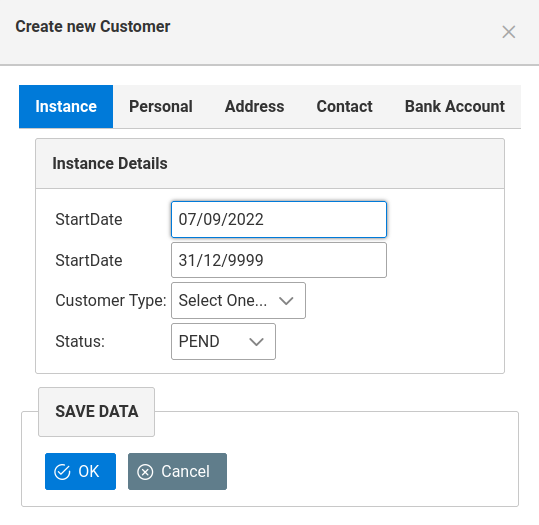
\includegraphics[width=0.50\textwidth]{imaxes/formulario-alta-cliente.png}
  \caption{Detalle del formulario de alta de clientes.}
  \label{fig:formulario-alta-cliente}
\end{figure}

Una vez finaliza la introducción de datos se pulsará el botón \emph{OK} que confirma la operación del formulario de creación. Si todo es correcto se registra el cliente en el sistema, se muestra un mensaje con el id del nuevo cliente creado y se muestran los datos del cliente creado la pantalla de visualización de la entidad.

Por defecto la fecha de Activación del cliente no se cubre, por lo que si queremos activar el cliente deberemos especificarla manualmente a través de la edición del registro del cliente creado.


\begin{figure}[H]
  \centering
  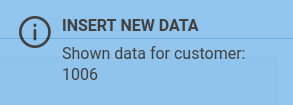
\includegraphics[width=0.3\textwidth]{imaxes/mensaje-id-cliente.png}
  \caption{Detalle del mensaje que informa del id del cliente creado.}
  \label{fig:mensaje-id-cliente}
\end{figure}


\item[\underline{\textsl{\textbf{Editar registro de histórico de cliente}}}] Esta operación sólo está disponible para usuarios con permisos de edición.
Para editar un registro de histórico se seleccionará el registro deseado del listado de históricos de la entidad y se pulsará el botón editar de la columna \textit{EDIT ROW} correspondiente. Se editarán los campos pertinentes directamente en la tabla para realizar las modificaciones oportunas teniendo en cuenta los criterios de fechas establecidos (definidos en la sección \ref{sub:histórico-conceptos} de la página \pageref{sub:histórico-conceptos}).

Al igual que para las entidades con históricos vistas en la sección del catálogo del sistema, si se cambia el estado de un cliente a cancelado, este cambio de estado se propagará a todos los registros posteriores al que cambiamos. Además se establecerá como fecha de cancelación la fecha en la que se realiza dicho cambio, propagándose ese dato por todos los registros de histórico del cliente, no sólo los que están a continuación del registro al que se le cambió el estado a cancelado.

Esta propagación de la fecha de cancelación por todos los registros del histórico  también ocurre si se modifica dicha fecha. Lo mismo ocurre si se cambia la fecha de activación del cliente.

\item[\underline{\textsl{\textbf{Añadir registro de histórico a un cliente}}}] Esta operación sólo está disponible para usuarios con permisos de edición.
Para añadir un nuevo registro de histórico sobre el cliente se seleccionará del listado el registro en el que se ubicará el nuevo registro a añadir y se pulsará el botón añadir de la columna \textit{ADD ROW} correspondiente. Aparecerá una nueva ventana emergente como la que se muestra en la operación de creación pero con los campos cubiertos con la información del registro sobre el que se va a añadir el nuevo registro y se realizán las moficaciones oportunas sobre los mismos teniendo en cuenta los criterios de fechas establecidos (definidos en la sección \ref{sub:histórico-conceptos} de la página \pageref{sub:histórico-conceptos}).


\item[\underline{\textsl{\textbf{Borrar registro de histórico del cliente }}}] Esta operación sólo está disponible para usuarios con permisos de edición.
Para borrar un registro de histórico del cliente se seleccionará del listado el registro a borrar y se pulsará el botón amarillo de borrar de la columna \textit{DEL ROW} correspondiente.

\item[\underline{\textsl{\textbf{Borrar el cliente}}}]
Esta operación sólo está disponible para usuarios con permisos de edición.
Para borrar completamente un cliente se deben borrar uno a uno todos los registros de histórico del cliente según lo indicado en el punto anterior.
\end{description}





\subsubsection{Account - Cuenta}
\label{sub:account}

Esta vista muestra la información relativa a las cuenta contenidas en la cartera de cuentas de la empresa.

Una cuenta depende de un cliente, por lo que existe una relación directa entre una cuenta y su cliente, no puede existir de forma independiente. Puesto que la cuenta es la entidad del sistema que permite gestionar los distintos productos y servicios contratados por el cliente y es la responsable de la transacción económica asociada a la contratación, esto es, el \textit{pagador}, tendrá asociada una persona física o jurídica que es la que efectuará el pago y que puede coincidir con el cliente o ser otra distinta. Por lo tanto el ciclo de facturación que aplicará sobre los distintos elementos contratados vendrá dado por la cuenta asociada a los mismos y vendrá dado por el tipo de cuenta asociado a la misma.


La \tablename~\ref{tab:cuenta} recoge los elementos más relevantes en la definición de una cuenta.
Las operaciones definidas para esta entidad son las siguientes:

\begin{table}
  \centering
  \rowcolors{2}{white}{udcgray!25}
  \setlength{\leftmargini}{0.4cm}
  \resizebox{14cm}{!} {
  \begin{tabular}{|m{5cm} m{9cm}|}
  \rowcolor{udcpink!25}
  \hline
  	\textbf{Elemento} & \textbf{Descripción} \\\hline
  	\textbf{START DATE} & Fecha de inicio del período temporal para el que aplican las condiciones especificadas para dicho período.\\
  	\textbf{END DATE} & Fecha de finalización del período temporal para el que aplican las condiciones especificadas para dicho período.\\
	\textbf{CUSTOMER ID} & Identificador unívoco del cliente al que está vinculado la cuenta.\\
	\textbf{ACCOUNT TYPE} & Tipo de cuenta asociado a la cuenta. Define la información relativa a la facturación.\\
	\textbf{ACCOUNT ID} & Identificador unívoco de la cuenta generado por la apliación.\\
	\textbf{CODE} & Código identificativo de la cuenta dentro del cliente. Sólo puede existir una cuenta con un código por cliente (aunque puede haber más cuentas con el mismo código identificativo para cuentas que pertenecen a distintos clientes).\\
	\textbf{CONTRACT NUMBER} & Número de contrato asociado a la cuenta. No puede haber más de una cuenta distinta con el mismo número de contrato..\\
	\textbf{NAME} & Nombre de la persona física o jurídica asociada a la cuenta.\\
	\textbf{1st SURNAME} & Primer apellido de la persona física o jurídica asociada a la cuenta.\\
	\textbf{2nd SURNAME} & Segundo apellido de la persona física o jurídica asociada a la cuenta.\\
	\textbf{IDENTITY CARD} & Número del documento de identificación de la persona física o jurídica asociada a la cuenta.\\	
	\textbf{ADDRESS}, \textbf{CITY}, \textbf{STATE}, \textbf{POST CODE}, \textbf{COUNTRY}  & Datos relativos a la dirección de de la persona física o jurídica asociada a la cuenta.\\	
	\textbf{CONTACT PHONE} & Número de teléfono de contacto de la persona física o jurídica asociada a la cuenta (no obligatorio).\\
	\textbf{EMAIL} & Dirección de correo electrónico de la persona física o jurídica asociada a la cuenta (no obligatorio).\\
	\textbf{IBAN}, \textbf{BANK ENTITY}, \textbf{BANK BRANCH}, \textbf{BANK CONTROL DIGIT}, \textbf{BANK ACCOUNT NUMBER} & Cuenta corriente de la persona física o jurídica asociada a la cuenta (no obligatorio).\\
	\textbf{ACTIVE DATE} & Fecha de activación de la cuenta. Común a todos los registros de histórico. Sólo cubierta cuando el cuenta se ha activado en el sistema.\\	
	\textbf{CANCELLED DATE} & Fecha de baja de la cuenta. Común a todos los registros de histórico. Sólo cubierta cuando el cuenta ha cursado baja (estado cancelado).	\\
	\textbf{STATUS} & Estado de la cuenta para el histórico actual.	
	\\\hline
  \end{tabular}
  } % end /resizebox
  \caption{Datos que definen un cuenta.}
  \label{tab:cuenta}
\end{table}

\begin{description}
\item[\underline{\textsl{\textbf{Buscar un cuenta existente}}}] Esta operación está disponible para todos los usuarios de la aplicación.
Se define un área de búsqueda en los que se definen los criterios de búsqueda a tener en cuenta:
\begin{itemize}
	\item Área Account Data: en este área se definen los criterios de búsqueda relativos a la propia cuenta:
	\begin{itemize}
		\item Contract Nr: número de contrato asociado a la cuenta.
		\item Account Id: identificador de la cuenta.
		\item Account Identity Card: número del documento de identificación de la cuenta (NIF, NIE\dots).
	\end{itemize}
	\item Área Customer Data: en este área se definen los criterios de búsqueda del cliente del que depende la cuenta.
	\begin{itemize}
		\item Customer Id: identificador del cliente asociado a la cuenta.
		\item Identity Card: número del documento de identificación del cliente asociado a la cuenta (NIF, NIE\dots).
	\end{itemize}
	\item Área Search Date: fecha de referencia de búsqueda. Se obtendrá como resultado el registro de histórico en el que esté comprendida dicha fecha. Este campo es obligatorio para realizar la búsqueda.
\end{itemize}

Una vez cubiertos los criterios indicados se pulsará el botón \emph{Search}, que mostrará un panel emergente con el listado de los registros encontrados. Seleccionaremos el elemento sobre el que queramos operar pulsando el botón amarillo de la columna \emph{Show Historic}. Se mostrará el área de históricos de la entidad con los distintos registros de histórico existentes.


\item[\underline{\textsl{\textbf{Crear nueva cuenta}}}] Esta operación sólo está habilitada para usuarios con permisos de edición.
Para crear una nueva cuenta se pulsará el botón \textit{New Data} situado en el área \emph{Create New Account} en la parte superior derecha de la ventana. Aparecerá una ventana emergente que mostrará un formulario con distintas pestañas relativas a la información a cubrir. A continuación se detallan dichas pestañas:
\begin{enumerate}
\item Pestaña Contract and Customer Data: en este apartado se define tanto el contrato asociado a la cuenta como el cliente del que depende. 
	\begin{itemize}
		\item Área Contract Data: Si queremos usar un contrato ya existente en el servicio introduciremos el número de contrato a relacionar en el campo de texto \emph{Contract Nr}. Si por el contrario queremos asociar un nuevo contrato pulsaremos el botón \emph{New Contract}, que generará un nuevo número de contrato y lo visualizará en el campo de texto \emph{Contract Nr}.
		\item Área Customer Data: Si sabemos el identificador del cliente del que dependerá la cuenta a crear, introduciremos ese valor en el campo \emph{Customer Id}. En caso contrario introduciremos el valor del documento identificativo del cliente a asociar en el área de texto Customer Identity Card y pulsaremos el botón search. Esto mostrará un listado con los clientes cuyo documento identificativo coincida con el introducido, seleccionaremos el cliente deseado y plusaremos el botón amarillo de la columna \emph{Select} correspondiente a dicho registro. Esto cargará la información del cliente en el área Custome Data.		
	\end{itemize}		
\item Pestaña Instance Details: aquí se define, entre otros, el tipo de cuenta que va a tener asociada esta cuenta. Los campos a definir son los siguientes y son todos obligatorios:
	\begin{itemize}
	\item Start Date: fecha de inicio del registro a crear (fecha desde la que queremos que la cuenta figure como registrado en el sistema). Por defecto aparece la fecha actual.
	\item End Date: fecha de fin del registro a crear. Por defecto aparece la máxima fecha del sistema (31/12/9999). Recomendamos no modificar esta fecha.
	\item Account Type: clasificación del tipo de cuenta con el que se va a dar de alta la nueva cuenta.
	\item Status: por defecto aparece el status pending, con vistas a la provisión, pero se puede seleccionar otro.
	\end{itemize}
\item Pestaña Personal: aquí se define la información relativa a la persona física o jurídica. Los campos a definir son los siguientes y son todos obligatorios:
	\begin{itemize}
	\item Name: nombre de la persona física o jurídia asociada a la cuenta.
	\item 1st Surname: primer apellido de la persona física o jurídia asociada a la cuenta.
	\item 2nd Surname: segundo apellido de la persona física o jurídia asociada a la cuenta.
	\item ID Card Type: tipo de documento de identificación de la persona física o jurídia asociada a la cuenta. Se seleccionará el que corresponda del listado.
	\item ID Card: número del documento de identificación de la persona física o jurídia asociada a la cuenta.
	\end{itemize}
\item Pestaña Address: aquí se define la información relativa a la dirección de la persona física o jurídia asociada a la cuenta a efectos de notificación. Los campos a definir son los siguientes y son todos obligatorios:
	\begin{itemize}
	\item Address: dirección: calle o vía, número, piso, puerta, etc.
	\item Post Code: código postal.
	\item City: Ciudad.
	\item State: Provincia.
	\item Country: País.
	\end{itemize}
\item Pestaña Contact: aquí se define la información de contacto de la persona física o jurídia asociada a la cuenta. Los campos a definir son los siguientes y no son obligatorios:
	\begin{itemize}
	\item Phone: número de teléfono de contacto.
	\item Email: dirección de correo electrónico.
	\end{itemize}
\item Pestaña Bank Account: aquí se define la información de la cuenta corriente de la persona física o jurídia asociada a la cuenta. Los campos a definir son los siguientes y no son obligatorios, pero si se cubren deben cubrirse todos:
	\begin{itemize}
	\item IBAN: número de Iban (4 caracteres alfanuméricos).
	\item Bank Entity: código del banco (4 dígitos).
	\item Bank Branch: código de entidad (4 dígitos).
	\item Bank Control Digit: dígito de control (2 dígitos).
	\item Bank Account Number: número de cuenta (10 dígitos).	
	\end{itemize}	
\end{enumerate}


\begin{figure}[H]
  \centering
  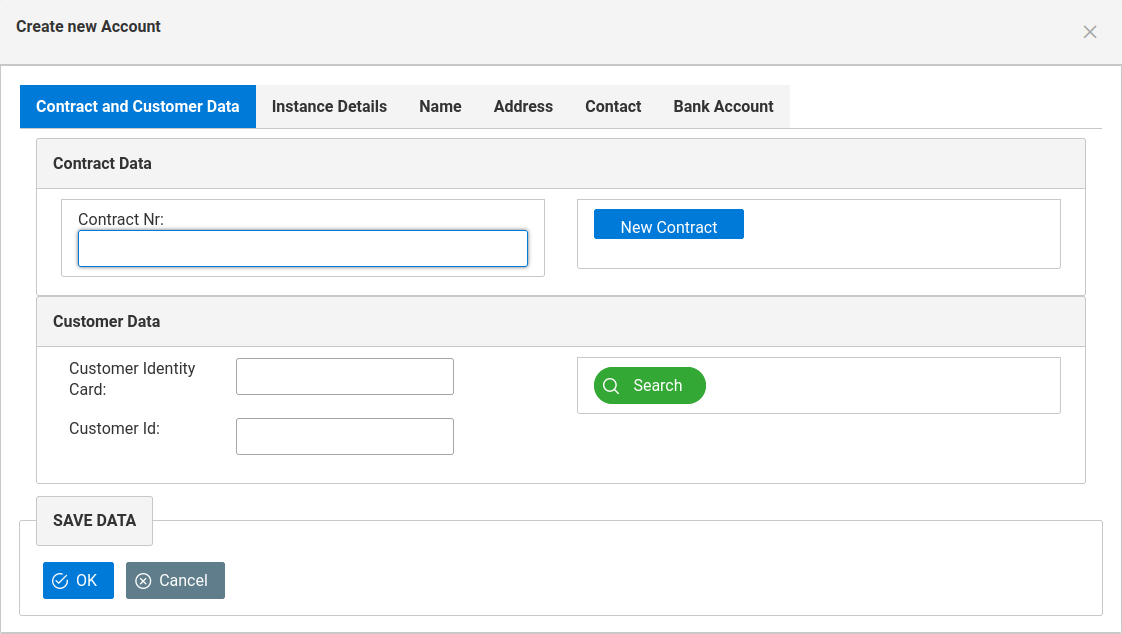
\includegraphics[width=0.9\textwidth]{imaxes/formulario-alta-cuenta.png}
  \caption{Detalle del formulario de alta de cuentas}
  \label{fig:formulario-alta-cuenta}
\end{figure}

Una vez finaliza la introducción de datos se pulsará el botón \emph{OK} que confirma la operación del formulario de creación. Si todo es correcto se registra el cuenta en el sistema, se muestra un mensaje con el id de la nueva cuenta creada y se muestran los datos de la cuenta creado la pantalla de visualización de la entidad.

Por defecto la fecha de Activación de la cuenta no se cubre, por lo que si queremos activar el cuenta deberemos especificarla manualmente a través de la edición del registro de la cuenta creada.


\begin{figure}[H]
  \centering
  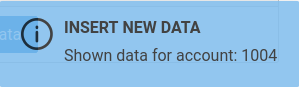
\includegraphics[width=0.35\textwidth]{imaxes/mensaje-id-cuenta.png}
  \caption{Detalle del mensaje que informa del id de la cuenta creado.}
  \label{fig:mensaje-id-cuenta}
\end{figure}


\item[\underline{\textsl{\textbf{Editar registro de histórico de cuenta}}}] Esta operación sólo está disponible para usuarios con permisos de edición.
Para editar un registro de histórico se seleccionará el registro deseado del listado de históricos de la entidad y se pulsará el botón editar de la columna \textit{EDIT ROW} correspondiente. Se editarán los campos pertinentes directamente en la tabla para realizar las modificaciones oportunas teniendo en cuenta los criterios de fechas establecidos (definidos en la sección \ref{sub:histórico-conceptos} de la página \pageref{sub:histórico-conceptos}).

Al igual que para las entidades con históricos vistas en la sección del catálogo del sistema, si se cambia el estado de un cuenta a cancelado, este cambio de estado se propagará a todos los registros posteriores al que cambiamos. Además se establecerá como fecha de cancelación la fecha en la que se realiza dicho cambio, propagándose ese dato por todos los registros de histórico de la cuenta, no sólo los que están a continuación del registro al que se le cambió el estado a cancelado.

Esta propagación de la fecha de cancelación por todos los registros del histórico  también ocurre si se modifica dicha fecha. Lo mismo ocurre si se cambia la fecha de activación de la cuenta.

\item[\underline{\textsl{\textbf{Añadir registro de histórico a un cuenta}}}] Esta operación sólo está disponible para usuarios con permisos de edición.
Para añadir un nuevo registro de histórico sobre el cuenta se seleccionará del listado el registro en el que se ubicará el nuevo registro a añadir y se pulsará el botón añadir de la columna \textit{ADD ROW} correspondiente. Aparecerá una nueva ventana emergente como la que se muestra en la operación de creación  con los campos cubiertos con la información del registro sobre el que se va a añadir el nuevo registro y se realizán las moficaciones oportunas sobre los mismos teniendo en cuenta los criterios de fechas establecidos (definidos en la sección \ref{sub:histórico-conceptos} de la página \pageref{sub:histórico-conceptos}).


\item[\underline{\textsl{\textbf{Borrar registro de histórico de la cuenta}}}] Esta operación sólo está disponible para usuarios con permisos de edición.
Para borrar un registro de histórico de la cuenta se seleccionará del listado el registro a borrar y se pulsará el botón amarillo de borrar de la columna \textit{DEL ROW} correspondiente.

\item[\underline{\textsl{\textbf{Borrar la cuenta}}}] Esta operación sólo está disponible para usuarios con permisos de edición.
Para borrar completamente un cuenta se deben borrar uno a uno todos los registros de histórico de la cuenta según lo indicado en el punto anterior. 
\end{description}




\subsubsection{Product Instance - Producto}
\label{sub:product}

Esta vista muestra la información relativa a los productos contenidas en la cartera de productos de la empresa.

Un producto es una entidad facturable, por lo que cada instancia del mismo deberá llevar asociado el tipo impositivo asociado según marca la ley. Además el producto debe estar relacionado con una de las cuentas existentes en el sistema, no puede existir de forma independiente.


La \tablename~\ref{tab:producto} recoge los elementos más relevantes en la definición de un producto:

\begin{table}[H]
  \centering
  \rowcolors{2}{white}{udcgray!25}
  \setlength{\leftmargini}{0.4cm}
  \resizebox{14cm}{!} {
  \begin{tabular}{|m{6cm} m{8cm}|}
  \rowcolor{udcpink!25}
  \hline
  	\textbf{Elemento} & \textbf{Descripción} \\\hline
  	\textbf{START DATE} & Fecha de inicio del período temporal para el que aplican las condiciones especificadas para dicho período.\\
  	\textbf{END DATE} & Fecha de finalización del período temporal para el que aplican las condiciones especificadas para dicho período.\\
	\textbf{PRODUCT TYPE} & Tipo de producto asociado al producto.\\
	\textbf{ACCOUNT ID} & Identificador unívoco de la cuenta a la que pertenece el producto.\\
	\textbf{CODE} & Código identificativo del producto. Por defecto es el mismo que el tipo de producto asociado.\\	
	\textbf{TAX TYPE} & Tipo impositivo defindo para el producto.\\
	\textbf{ACTIVE DATE} & Fecha de activación del producto. Común a todos los registros de histórico. Sólo cubierta cuando el producto se ha activado en el sistema.\\	
	\textbf{CANCELLED DATE} & Fecha de baja del producto. Común a todos los registros de histórico. Sólo cubierta cuando el producto ha cursado baja (estado cancelado).	\\
	\textbf{STATUS} & Estado del producto para el histórico actual.	
	\\\hline
  \end{tabular}
  } % end /resizebox
  \caption{Datos que definen un producto.}
  \label{tab:producto}
\end{table}



Las operaciones definidas para esta entidad son las siguientes:

\begin{description}
\item[\underline{\textsl{\textbf{Buscar un producto existente}}}] Esta operación está disponible para todos los usuarios de la aplicación.
Se define un área de búsqueda en los que se definen los criterios de búsqueda a tener en cuenta:
\begin{itemize}
	\item Área Account Data: en este área se definen los criterios de búsqueda relativos a la cuenta a la que está asociado el producto:
	\begin{itemize}
		\item Contract Nr: número de contrato asociado a la cuenta.
		\item Account Id: identificador de la cuenta.
		\item Account Identity Card: número del documento de identificación de la cuenta (NIF, NIE\dots).
	\end{itemize}
	\item Área Customer Data: en este área se definen los criterios de búsqueda del cliente del que depende la cuenta asociada al producto.
	\begin{itemize}
		\item Customer Id: identificador del cliente asociado a la cuenta.
		\item Identity Card: número del documento de identificación del cliente asociado a la cuenta (NIF, NIE\dots).
	\end{itemize}
	\item Área Search Date: fecha de referencia de búsqueda. Se obtendrá como resultado el registro de histórico en el que esté comprendida dicha fecha. Este campo es obligatorio para realizar la búsqueda.
\end{itemize}

Una vez cubiertos los criterios indicados se pulsará el botón \emph{Search}, que mostrará un panel emergente con el listado de los registros encontrados. Seleccionaremos el elemento sobre el que queramos operar pulsando el botón amarillo de la columna \emph{Show Historic}. Se mostrará el área de históricos de la entidad con los distintos registros de histórico existentes.


\item[\underline{\textsl{\textbf{Crear nueva producto}}}] Esta operación sólo está habilitada para usuarios con permisos de edición.
Para crear una nueva producto se pulsará el botón \textit{New Data} situado en el área \emph{Create New Product} en la parte superior derecha de la ventana. Aparecerá una ventana emergente que mostrará dos partes diferenciadas. Un área superior denominada \emph{Parent Data} correspondiente a la cuenta asociada al producto y una parte inferior que se corresponde con los datos de la instancia del producto.

Si sabemos el id de la cuenta a la que vamos a asociar el producto la especificaremos en el área de texto \emph{Account Id} del área \emph{Account Criteria} del apartado \emph{Parent Data}. En caso de no saber el id procederemos a cubrir alguno de los campos del formulario del apartado \emph{Parent Data} y pulsaremos el botón \emph{Search}. Aparecerá un listado con todas las cuentas resultado de la búsqueda. Seleccionaremos el registro deseado y pulsaremos el botón amarillo de la columna \emph{Select} correspondiente. Se cargará la información correspondiente en el apartado \emph{Parent Data}.

A continuación cubriremos el resto de los datos correspondientes al producto a crear y que se encuentran debajo del apartado apartado \emph{Parent Data}:
\begin{itemize}
	\item Start Date: fecha de inicio del registro a crear (fecha desde la que queremos que el producto figure como registrado en el sistema). Por defecto aparece la fecha actual.
	\item End Date: fecha de fin del registro a crear. Por defecto aparece la máxima fecha del sistema (31/12/9999). Recomendamos no modificar esta fecha.
	\item Tax Type: Tipo impositivo a aplicar al producto a efectos de facturación.
	\item Product Type: tipo de producto al que pertenece el producto a crear.
	\item Status: por defecto aparece el status pending, con vistas a la provisión, pero se puede seleccionar otro.
\end{itemize}


\begin{figure}[H]
  \centering
  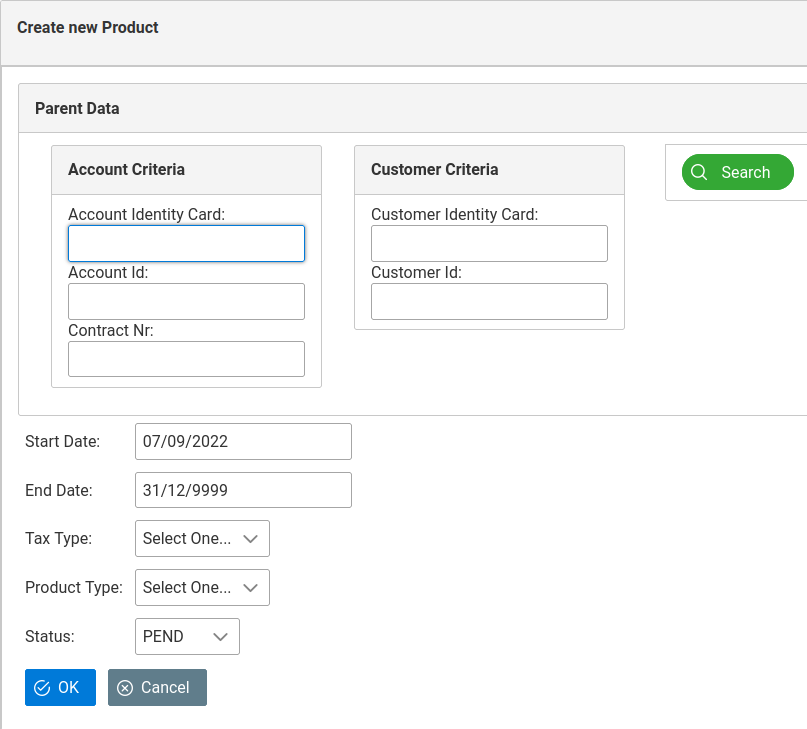
\includegraphics[width=0.70\textwidth]{imaxes/formulario-alta-producto.png}
  \caption{Detalle del formulario de alta de productos}
  \label{fig:formulario-alta-producto}
\end{figure}

Una vez finaliza la introducción de datos se pulsará el botón \emph{OK} que confirma la operación del formulario de creación. Si todo es correcto se registra el producto en el sistema y se muestran los datos del producto creado la pantalla de visualización de la entidad.

Por defecto la fecha de Activación del producto no se cubre, por lo que si queremos activar el producto deberemos especificarla manualmente a través de la edición del registro del producto creada.


\item[\underline{\textsl{\textbf{Editar registro de histórico de producto}}}] Esta operación sólo está disponible para usuarios con permisos de edición.
Para editar un registro de histórico se seleccionará el registro deseado del listado de históricos de la entidad y se pulsará el botón editar de la columna \textit{EDIT ROW} correspondiente. Se editarán los campos pertinentes directamente en la tabla para realizar las modificaciones oportunas teniendo en producto los criterios de fechas establecidos (definidos en la sección \ref{sub:histórico-conceptos} de la página \pageref{sub:histórico-conceptos}).

Al igual que para las entidades con históricos vistas en la sección del catálogo del sistema, si se cambia el estado de un producto a cancelado, este cambio de estado se propagará a todos los registros posteriores al que cambiamos. Además se establecerá como fecha de cancelación la fecha en la que se realiza dicho cambio, propagándose ese dato por todos los registros de histórico del producto, no sólo los que están a continuación del registro al que se le cambió el estado a cancelado.

Esta propagación de la fecha de cancelación por todos los registros del histórico  también ocurre si se modifica dicha fecha. Lo mismo ocurre si se cambia la fecha de activación del producto.

\item[\underline{\textsl{\textbf{Añadir registro de histórico a un producto}}}] Esta operación sólo está disponible para usuarios con permisos de edición.
Para añadir un nuevo registro de histórico sobre el producto se seleccionará del listado el registro en el que se ubicará el nuevo registro a añadir y se pulsará el botón añadir de la columna \textit{ADD ROW} correspondiente. Aparecerá una nueva ventana emergente como la que se muestra en la operación de creación sin el área de búsqueda \emph{Parent Data} y con los campos cubiertos con la información del registro sobre el que se va a añadir el nuevo registro y se realizán las moficaciones oportunas sobre los mismos teniendo en servicio los criterios de fechas establecidos (definidos en la sección \ref{sub:histórico-conceptos} de la página \pageref{sub:histórico-conceptos}). En la \figurename~\ref{fig:nuevo-historico-producto} se puede ver un detalle del formulario correspondiente.

\begin{figure}
  \centering
  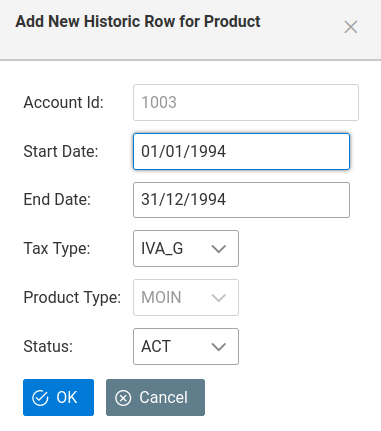
\includegraphics[width=0.4\textwidth]{imaxes/nuevo-historico-producto.png}
  \caption{Detalle del formulario para añadir un nuevo registro de histórico de producto}
  \label{fig:nuevo-historico-producto}
\end{figure}


\item[\underline{\textsl{\textbf{Borrar registro de histórico del producto}}}] Esta operación sólo está disponible para usuarios con permisos de edición.
Para borrar un registro de histórico del producto se seleccionará del listado el registro a borrar y se pulsará el botón amarillo de borrar de la columna \textit{DEL ROW} correspondiente.

\item[\underline{\textsl{\textbf{Borrar el producto}}}] Esta operación sólo está disponible para usuarios con permisos de edición.
Para borrar completamente un producto se deben borrar uno a uno todos los registros de histórico del producto según lo indicado en el punto anterior. 
\end{description}


\subsubsection{Service Instance - Servicio}
\label{sub:service}

Esta vista muestra la información relativa a los servicios contenidas en la cartera de servicios de la empresa.

Un servicio es una entidad facturable, por lo que cada instancia del mismo deberá llevar asociado el tipo impositivo asociado según marca la ley. Además un servicio debe estar asociado a uno de los productos existentes en el sistema, no puede existir de forma independiente.

\begin{table}
  \centering
  \rowcolors{2}{white}{udcgray!25}
  \setlength{\leftmargini}{0.4cm}
  \resizebox{14cm}{!} {
  \begin{tabular}{|m{4.5cm} m{11cm}|}
  \rowcolor{udcpink!25}
  \hline
  	\textbf{Elemento} & \textbf{Descripción} \\\hline
  	\textbf{START DATE} & Fecha de inicio del período temporal para el que aplican las condiciones especificadas para dicho período.\\
  	\textbf{END DATE} & Fecha de finalización del período temporal para el que aplican las condiciones especificadas para dicho período.\\
	\textbf{PRODUCT ID} & Identificador unívoco del producto al que está vinculado el servicio.\\
	\textbf{SERVICE TYPE} & Tipo de servicio asociado al servicio.\\
	\textbf{SERVICE NUMBER} & Número que identifica al servicio. Sólo debe existir un servicio con estado distinto de cancelado en el sistema con ese número.\\
	\textbf{GENERAL 1}, \textbf{GENERAL 2}, \textbf{GENERAL 3} & Campos generales que contienen información adicional del servicio (no definidos).\\	
	\textbf{TAX TYPE} & Tipo impositivo defindo para el servicio.\\
	\textbf{ACTIVE DATE} & Fecha de activación del servicio. Común a todos los registros de histórico. Sólo cubierta cuando el servicio se ha activado en el sistema.\\	
	\textbf{CANCELLED DATE} & Fecha de baja del servicio. Común a todos los registros de histórico. Sólo cubierta cuando el servicio ha cursado baja (estado cancelado).	\\
	\textbf{STATUS} & Estado del servicio para el histórico actual.	
	\\\hline
  \end{tabular}
  } % end /resizebox
  \caption{Datos que definen un servicio.}
  \label{tab:servicio}
\end{table}

La \tablename~\ref{tab:servicio} recoge los elementos más relevantes en la definición de un servicio.
Las operaciones definidas para esta entidad son las siguientes:
\begin{description}
\item[\underline{\textsl{\textbf{Buscar un servicio existente}}}] Esta operación está disponible para todos los usuarios de la aplicación.
Se define un área de búsqueda en los que se definen los criterios de búsqueda a tener en cuenta:
\begin{itemize}
	\item Área Account Data: en este área se definen los criterios de búsqueda relativos a la cuenta a la que está asociado el servicio:
		\begin{itemize}
			\item Contract Nr: número de contrato asociado a la cuenta.
			\item Account Id: identificador de la cuenta.
			\item Account Identity Card: número del documento de identificación de la cuenta (NIF, NIE\dots).
		\end{itemize}
	\item Área Customer Data: en este área se definen los criterios de búsqueda del cliente del que depende la cuenta asociada al servicio.
		\begin{itemize}
			\item Customer Id: identificador del cliente asociado a la cuenta.
			\item Identity Card: número del documento de identificación del cliente asociado a la cuenta (NIF, NIE\dots).
		\end{itemize}
	\item Área Product Data: en este área se definen los criterios de búsqueda del producto del que depende el servicio. Está pensada para completar la búsqueda con otra información aportada en el resto de áreas.	
		\begin{itemize}
			\item Product Id: identificador del producto.
			\item Product Type: tipo del producto.
		\end{itemize}
	\item Área Service Data: en este área se definen los criterios de búsqueda del servicio.
		\begin{itemize}
			\item Service Nr: número del servicio a buscar.
			\item Product Type: tipo del servicio a buscar. Está pensada para completar la búsqueda con otra información aportada en el resto de áreas.
		\end{itemize}
	\item Área Search Date: fecha de referencia de búsqueda. Se obtendrá como resultado el registro de histórico en el que esté comprendida dicha fecha. Este campo es obligatorio para realizar la búsqueda.
\end{itemize}

Una vez cubiertos los criterios indicados se pulsará el botón \emph{Search}, que mostrará un panel emergente con el listado de los registros encontrados. Seleccionaremos el elemento sobre el que queramos operar pulsando el botón amarillo de la columna \emph{Show Historic}. Se mostrará el área de históricos de la entidad con los distintos registros de histórico existentes.

\item[\underline{\textsl{\textbf{Crear nueva servicio}}}] Esta operación sólo está habilitada para usuarios con permisos de edición.
Para crear una nueva servicio se pulsará el botón \textit{New Data} situado en el área \emph{Create New Service} en la parte superior derecha de la ventana. Aparecerá una ventana emergente que mostrará dos partes diferenciadas. Un área superior denominada \emph{Parent Data} correspondiente al producto asociado al servicio y una parte inferior que se corresponde con los datos de la instancia del servicio.

Si sabemos el id del producto a la que vamos a asociar el servicio la especificaremos en el área de texto \emph{Product Id} del área \emph{Product Criteria} del apartado \emph{Parent Data}. En caso de no saber el id procederemos a cubrir alguno de los campos del formulario del apartado \emph{Parent Data} de forma análoga a lo realizado para especificar los criterios de búsquda del servicio y pulsaremos el botón \emph{Search}. Aparecerá un listado con todos los productos resultado de la búsqueda. Seleccionaremos el registro deseado y pulsaremos el botón amarillo de la columna \emph{Select} correspondiente. Se cargará la información correspondiente en el apartado \emph{Parent Data}.

A continuación cubriremos el resto de los datos correspondientes al servicio a crear y que se encuentran debajo del apartado apartado \emph{Parent Data}:
\begin{itemize}
	\item Start Date: fecha de inicio del registro a crear (fecha desde la que queremos que el servicio figure como registrado en el sistema). Por defecto aparece la fecha actual.
	\item End Date: fecha de fin del registro a crear. Por defecto aparece la máxima fecha del sistema (31/12/9999). Recomendamos no modificar esta fecha.
	\item Tax Type: Tipo impositivo a aplicar al servicio a efectos de facturación.
	\item Service Type: tipo de servicio al que pertenece el servicio a crear.	
		\item Fee Type: tipo de servicio a crear. 
	\item General 1: campo reservado a información adicional. Puede dejarse sin cubrir.
	\item General 2: campo reservado a información adicional. Puede dejarse sin cubrir.
	\item General 3: campo reservado a información adicional. Puede dejarse sin cubrir.
	\item Status: por defecto aparece el status pending, con vistas a la provisión, pero se puede seleccionar otro.
\end{itemize}

Una vez finaliza la introducción de datos se pulsará el botón \emph{OK} que confirma la operación del formulario de creación. Si todo es correcto se registra el servicio en el sistema y se muestran los datos del servicio creado la pantalla de visualización de la entidad.

Por defecto la fecha de Activación del servicio no se cubre, por lo que si queremos activar el servicio deberemos especificarla manualmente a través de la edición del registro del servicio creada.

La \figurename~\ref{fig:formulario-alta-servicio} muestra un detalle del formulario de alta de servicios.

\begin{figure}
  \centering
  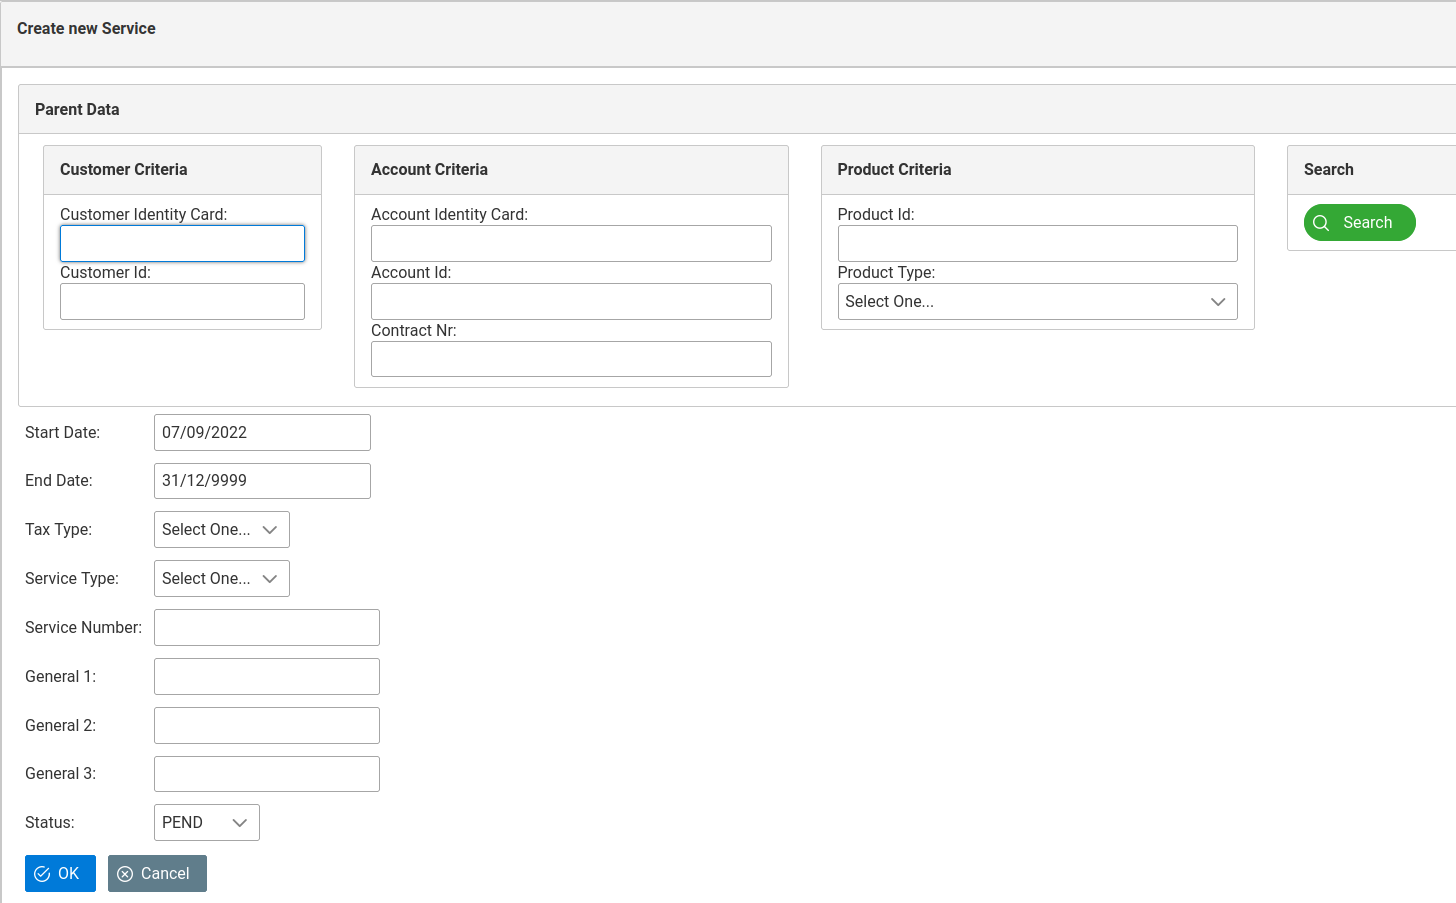
\includegraphics[width=0.9\textwidth]{imaxes/formulario-alta-servicio.png}
  \caption{Detalle del formulario de alta de servicios}
  \label{fig:formulario-alta-servicio}
\end{figure}


\item[\underline{\textsl{\textbf{Editar registro de histórico de servicio}}}] Esta operación sólo está disponible para usuarios con permisos de edición.
Para editar un registro de histórico se seleccionará el registro deseado del listado de históricos de la entidad y se pulsará el botón editar de la columna \textit{EDIT ROW} correspondiente. Se editarán los campos pertinentes directamente en la tabla para realizar las modificaciones oportunas teniendo en servicio los criterios de fechas establecidos (definidos en la sección \ref{sub:histórico-conceptos} de la página \pageref{sub:histórico-conceptos}).

Al igual que para las entidades con históricos vistas en la sección del catálogo del sistema, si se cambia el estado de un servicio a cancelado, este cambio de estado se propagará a todos los registros posteriores al que cambiamos. Además se establecerá como fecha de cancelación la fecha en la que se realiza dicho cambio, propagándose ese dato por todos los registros de histórico del servicio, no sólo los que están a continuación del registro al que se le cambió el estado a cancelado.

Esta propagación de la fecha de cancelación por todos los registros del histórico  también ocurre si se modifica dicha fecha. Lo mismo ocurre si se cambia la fecha de activación del servicio.

\item[\underline{\textsl{\textbf{Añadir registro de histórico a un servicio}}}] Esta operación sólo está disponible para usuarios con permisos de edición.
Para añadir un nuevo registro de histórico sobre el servicio se seleccionará del listado el registro en el que se ubicará el nuevo registro a añadir y se pulsará el botón añadir de la columna \textit{ADD ROW} correspondiente. Aparecerá una nueva ventana emergente como la que se muestra en la operación de creación sin el área de búsqueda \emph{Parent Data} y con los campos cubiertos con la información del registro sobre el que se va a añadir el nuevo registro y se realizán las moficaciones oportunas sobre los mismos teniendo en servicio los criterios de fechas establecidos (definidos en la sección \ref{sub:histórico-conceptos} de la página \pageref{sub:histórico-conceptos}).

La \figurename~\ref{fig:nuevo-historico-servicio} muestra un detalle del formulario para añadir un nuevo registro al histórico de un servicio:

\begin{figure}[H]
  \centering
  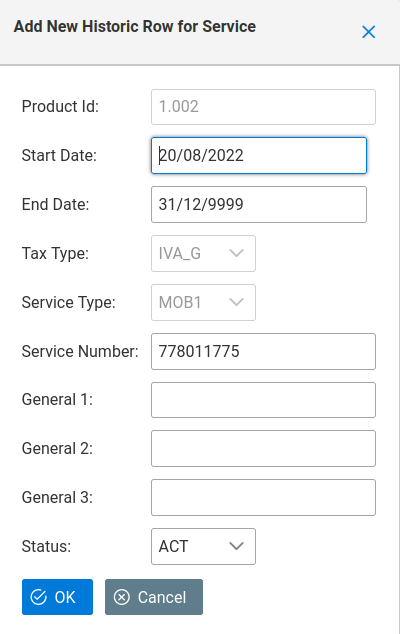
\includegraphics[width=0.40\textwidth]{imaxes/nuevo-historico-servicio.png}
  \caption{Detalle del formulario para añadir un nuevo registro de histórico de servicio}
  \label{fig:nuevo-historico-servicio}
\end{figure}


\item[\underline{\textsl{\textbf{Borrar registro de histórico del servicio}}}] Esta operación sólo está disponible para usuarios con permisos de edición.
Para borrar un registro de histórico del servicio se seleccionará del listado el registro a borrar y se pulsará el botón amarillo de borrar de la columna \textit{DEL ROW} correspondiente.

\item[\underline{\textsl{\textbf{Borrar el servicio}}}] Esta operación sólo está disponible para usuarios con permisos de edición.
Para borrar completamente un servicio se deben borrar uno a uno todos los registros de histórico del servicio según lo indicado en el punto anterior. 
\end{description}


\subsubsection{Fee Instance - Cuota}
\label{sub:fee}

Esta vista muestra la información relativa a las cuotas contenidas en la cartera de servicios de la empresa.

Una cuota debe estar asociado a un producto o servicio existentes en el sistema, no puede existir de forma independiente.

Aunque los valores de prorrateo y precio de la cuota vienen definidos por el tipo de cuota asociado a la cuota contratada, estos valores pueden cambiar en la cuota, para adaptarse a las necesidades del cliente.


\begin{table}
  \centering
  \rowcolors{2}{white}{udcgray!25}
  \setlength{\leftmargini}{0.4cm}
  \resizebox{14cm}{!} {
  \begin{tabular}{|m{4cm} m{11cm}|}
  \rowcolor{udcpink!25}
  \hline
  	\textbf{Elemento} & \textbf{Descripción} \\\hline
  	\textbf{START DATE} & Fecha de inicio del período temporal para el que aplican las condiciones especificadas para dicho período.\\
  	\textbf{END DATE} & Fecha de finalización del período temporal para el que aplican las condiciones especificadas para dicho período.\\
	\textbf{PARENT ID} & Identificador unívoco de la instancia a la que está vinculada la cuota (product\_id si la cuota aplica a nivel de producto o service\_id si aplica a nivel de servicio).\\
	\textbf{CODE} & Código identificativo de la cuota. Por defecto es el mismo que el tipo de cuota asociado.\\	
	\textbf{FEE TYPE} & Tipo de cuota asociado a la cuota.\\
	\textbf{APPLICATION LEVEL} & Nivel de aplicación de la cuota (producto o servicio). Viene dado por su tipo de cuota.\\
	\textbf{PRORRATE} & Indica si la cuota es prorrateable (\textit{TRUE}) o no (\textit{FALSE}). Se toma como base el importe definido en el tipo de cuota, pero puede variar para adaptarse a las necesidades del cliente.\\
	\textbf{PRICE} & Indica el importe a facturar por dicha cuota. Se toma como base el importe definido en el tipo de cuota, pero puede variar para adaptarse a las necesidades del cliente.\\
	\textbf{ACTIVE DATE} & Fecha de activación de la cuota. Común a todos los registros de histórico. Sólo cubierta cuando la cuota se ha activado en el sistema.\\
	\textbf{CANCELLED DATE} & Fecha de baja de la cuota. Común a todos los registros de histórico. Sólo cubierta cuando la cuota ha cursado baja (estado cancelado).\\
	\textbf{STATUS} & Estado de la cuota para el histórico actual.	
	\\\hline
  \end{tabular}
  } % end /resizebox
  \caption{Datos que definen una cuota.}
  \label{tab:cuota}
\end{table}

La \tablename~\ref{tab:cuota} recoge los elementos más relevantes en la definición de una cuota.
Las operaciones definidas para esta entidad son las siguientes:

\begin{description}
\item[\underline{\textsl{\textbf{Buscar una cuota existente}}}] Esta operación está disponible para todos los usuarios de la aplicación.
Se define un área de búsqueda en los que se definen los criterios de búsqueda a tener en cuenta:
\begin{itemize}
	\item Área Account Data: en este área se definen los criterios de búsqueda relativos a la cuenta a la que está asociada la cuota:
		\begin{itemize}
			\item Contract Nr: número de contrato asociado a la cuenta.
			\item Account Id: identificador de la cuenta.
			\item Account Identity Card: número del documento de identificación de la cuenta (NIF, NIE\dots).
		\end{itemize}
	\item Área Customer Data: en este área se definen los criterios de búsqueda del cliente del que depende la cuenta asociada a la cuota.
		\begin{itemize}
			\item Customer Id: identificador del cliente asociado a la cuenta.
			\item Identity Card: número del documento de identificación del cliente asociado a la cuenta (NIF, NIE\dots).
		\end{itemize}
	\item Área Paren Instance: en este área se definen los criterios de búsqueda de la entidad padre de la cuota. Para ello se selecciona el nivel de aplicación de la cuota a buscar. Se puede completar la búsqueda aportando información relativa a la entidad padre a la que está asociada la cuenta, para lo que se definen unos campos a cubrir. En función de si se ha seleccionado producto o servicio se muestran distintos campos:
	\begin{itemize}
 		\item \emph{Application Level: PRODUCTO} seleccionado: se mostrarán los siguientes campos a cubrir:
			\begin{itemize}
				\item Product Id: identificador del producto al que está asociado la cuota.
				\item Product Type: tipo del producto al que está asociado la cuota.
			\end{itemize}
		\item \emph{Application Level: SERVICE} seleccionado:  se mostrarán los siguientes campos a cubrir:
		\begin{itemize}
			\item Service Nr: número de servicio del servicio al que está asociado la cuota.
			\item Product Type: tipo de servicio del servicio al que está asociado la cuota.
		\end{itemize}
		
	\end{itemize}	    	
	\item Área Search Date: fecha de referencia de búsqueda. Se obtendrá como resultado el registro de histórico en el que esté comprendida dicha fecha. Este campo es obligatorio para realizar la búsqueda.
\end{itemize}

Una vez cubiertos los criterios indicados se pulsará el botón \emph{Search}, que mostrará un panel emergente con el listado de los registros encontrados para las cuotas que cumplan los criterios de búsqueda especificados. Seleccionaremos el elemento sobre el que queramos operar pulsando el botón amarillo de la columna \emph{Show Historic}. Se mostrará el área de históricos de la entidad con los distintos registros de histórico existentes.


\item[\underline{\textsl{\textbf{Crear nueva cuota}}}] Esta operación sólo está habilitada para usuarios con permisos de edición.
Para crear una nueva servicio se pulsará el botón \textit{New Data} situado en el área \emph{Create New Fee} en la parte superior derecha de la ventana. Aparecerá una ventana emergente que mostrará dos partes diferenciadas. Un área superior denominada \emph{Search Parent Data} minimizada correspondiente a la jerarquía de la entidad producto o servicio asociada a la cuota a crear y una parte inferior que se corresponde con los datos de la instancia de la cuota.

Si sabemos el id de la entidad a la que vamos a asociar la cuota la especificaremos en el área de texto \emph{Parent Id}. En caso de no saber el id procederemos a realizar la correspondiente búsqueda en el área  \emph{Search Parent Data}. Para ello desplegaremos ese área pulsando sobre \emph{Search Parent Data} y procederemos a cubrir alguno de los campos del formulario del apartado \emph{Search Parent Data} de forma análoga a lo realizado para especificar los criterios de búsquda de la cuota y pulsaremos el botón \emph{Search}. Aparecerá un listado con todos los productos o servicios (en función del nivel de aplicación seleccionado) resultado de la búsqueda. Seleccionaremos el registro deseado y pulsaremos el botón amarillo de la columna \emph{Select} correspondiente. Se cargará la información correspondiente en el apartado \emph{Search Parent Data}, así como los datos de \emph{Application Level} y \emph{Parent Id} del área de datos de la instancia de la cuota a crear.

A continuación cubriremos el resto de los datos correspondientes a la cuota a crear y que se encuentran debajo del apartado \emph{Search Parent Data} (importante: si el apartado \emph{Search Parent Data} está desplegado es posible que no se vea todo el formulario de creación de la cuota, por lo que habrá que minimizarlo pulsando en el nombre del apartado (\emph{Search Parent Data})).
\begin{itemize}
	\item Start Date: fecha de inicio del registro a crear (fecha desde la que queremos que la cuota figure como registrado en el sistema). Por defecto aparece la fecha actual.
	\item End Date: fecha de fin del registro a crear. Por defecto aparece la máxima fecha del sistema (31/12/9999). Recomendamos no modificar esta fecha.
	\item Application Level Id: Nivel de aplicación de la cuota. Si se ha recurrido al apartado \emph{Search Parent Data} del formulario para buscar la entidad con la que se va a relacionar la cuota, este campo se cubrirá de forma automática. 
	\item Parent Id: Identificador de la entidad padre a asociar la cuota. Si se ha recurrido al apartado \emph{Search Parent Data} del formulario para buscar la entidad con la que se va a relacionar la cuota, este campo se cubrirá de forma automática. 
	\item Fee Type: tipo de servicio a crear. La información mostrada en el desplegable se cubre en función de los datos del nivel de aplicación y del tipo asociado al Parent Id especificado y viene determinado por las relaciones de tipos de cuota establecidas en el catálogo de servicio para el tipo de entidad padre de la cuota a crear.
	\item Code: código asociado a la cuota.
	\item Prorrate: define si la cuota a crear será prorrateable (\textit{TRUE}) o no (\textit{FALSE}).
	\item Price: precio de la cuota a crear.
	\item Status: por defecto aparece el status pending, con vistas a la provisión, pero se puede seleccionar otro.
\end{itemize}



\begin{figure}
  \centering
  \begin{subfigure}[b]{0.3\textwidth}
    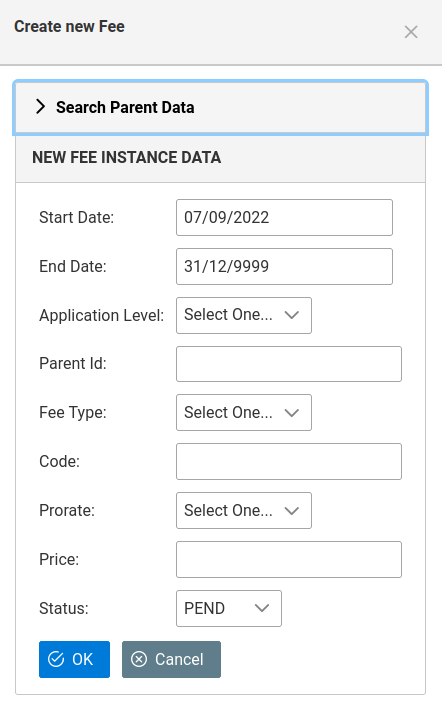
\includegraphics[width=\textwidth]{imaxes/formulario-alta-cuota-01.png}
    \caption{Sin el área de \emph{Search Parent Data} desplegada}
    \label{fig:formulario-alta-cuota-01}
  \end{subfigure}
%  \hspace{0.1\textwidth}
  \begin{subfigure}[b]{0.69\textwidth}
    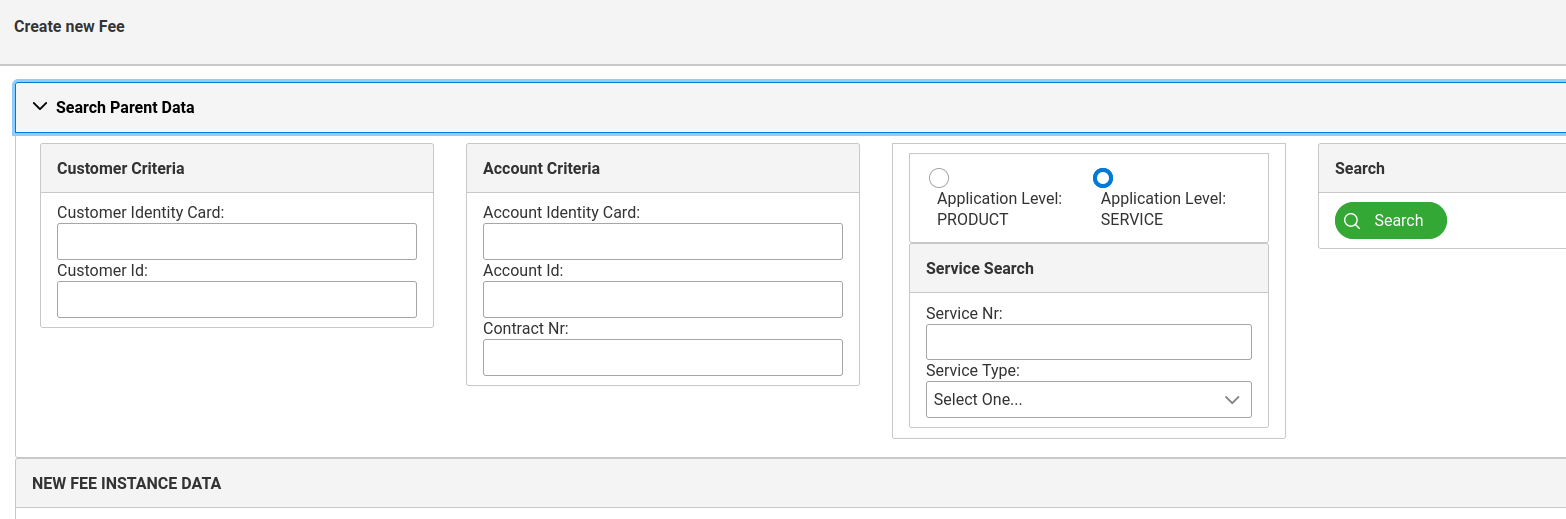
\includegraphics[width=\textwidth,height=3cm]{imaxes/formulario-alta-cuota-02.png}
    \caption{Con el área de \emph{Search Parent Data} desplegada}
    \label{fig:formulario-alta-cuota-02}
  \end{subfigure}
  \caption{Detalles del formulario de alta de cuota}
  \label{fig:alta-cuota}
\end{figure}


Una vez finaliza la introducción de datos se pulsará el botón \emph{OK} que confirma la operación del formulario de creación. Si todo es correcto se registra la cuota en el sistema y se muestran los datos de la cuota creado la pantalla de visualización de la entidad.

Por defecto la fecha de Activación de la cuota no se cubre, por lo que si queremos activar la cuota deberemos especificarla manualmente a través de la edición del registro de la cuota creada.

La \figurename~\ref{fig:alta-cuota} muestra dos detalles del formulario para añadir una nueva cuota, con y sin el \emph{Search Parent Data} desplegado.

\item[\underline{\textsl{\textbf{Editar registro de histórico de servicio}}}] Esta operación sólo está disponible para usuarios con permisos de edición.
Para editar un registro de histórico se seleccionará el registro deseado del listado de históricos de la entidad y se pulsará el botón editar de la columna \textit{EDIT ROW} correspondiente. Se editarán los campos pertinentes directamente en la tabla para realizar las modificaciones oportunas teniendo en servicio los criterios de fechas establecidos (definidos en la sección \ref{sub:histórico-conceptos} de la página \pageref{sub:histórico-conceptos}).

Al igual que para las entidades con históricos vistas en la sección del catálogo del sistema, si se cambia el estado de una cuota a cancelado, este cambio de estado se propagará a todos los registros posteriores al que cambiamos. Además se establecerá como fecha de cancelación la fecha en la que se realiza dicho cambio, propagándose ese dato por todos los registros de histórico de la cuota, no sólo los que están a continuación del registro al que se le cambió el estado a cancelado.

Esta propagación de la fecha de cancelación por todos los registros del histórico  también ocurre si se modifica dicha fecha. Lo mismo ocurre si se cambia la fecha de activación de la cuota.

\item[\underline{\textsl{\textbf{Añadir registro de histórico a una cuota}}}] Esta operación sólo está disponible para usuarios con permisos de edición.
Para añadir un nuevo registro de histórico sobre la cuota se seleccionará del listado el registro en el que se ubicará el nuevo registro a añadir y se pulsará el botón añadir de la columna \textit{ADD ROW} correspondiente. Aparecerá una nueva ventana emergente como la que se muestra en la operación de creación sin el área de búsqueda \emph{Parent Data} y con los campos cubiertos con la información del registro sobre el que se va a añadir el nuevo registro y se realizán las moficaciones oportunas sobre los mismos teniendo en servicio los criterios de fechas establecidos (definidos en la sección \ref{sub:histórico-conceptos} de la página \pageref{sub:histórico-conceptos}).

La \figurename~\ref{fig:nuevo-historico-cuota} muestra un detalle del formulario para añadir un nuevo registro al histórico de una cuota:

\begin{figure}[H]
  \centering
  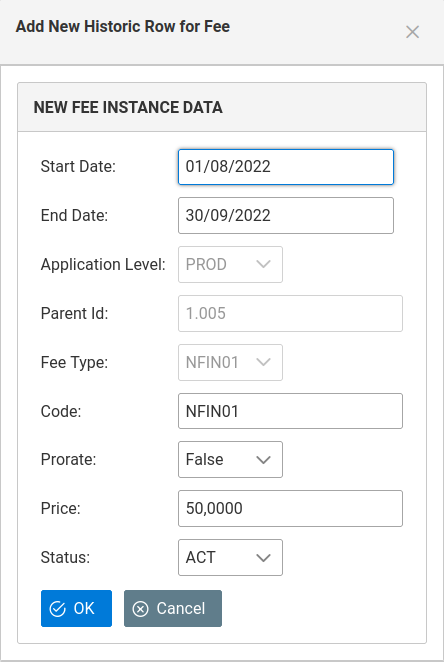
\includegraphics[width=0.425\textwidth]{imaxes/nuevo-historico-cuota.png}
  \caption{Detalle del formulario para añadir un nuevo registro de histórico de cuota}
  \label{fig:nuevo-historico-cuota}
\end{figure}



\item[\underline{\textsl{\textbf{Borrar registro de histórico de la cuota}}}] Esta operación sólo está disponible para usuarios con permisos de edición.
Para borrar un registro de histórico de la cuota se seleccionará del listado el registro a borrar y se pulsará el botón amarillo de borrar de la columna \textit{DEL ROW} correspondiente.

\item[\underline{\textsl{\textbf{Borrar la cuota}}}] Esta operación sólo está disponible para usuarios con permisos de edición.
Para borrar completamente una cuota se deben borrar uno a uno todos los registros de histórico de la cuota según lo indicado en el punto anterior. 
\end{description}



\subsubsection{Promotion Instance - Promoción}
\label{sub:promotion}

Esta vista muestra la información relativa a las promociones contenidas en la cartera de servicios de la empresa.

Una promoción debe estar asociado a un producto o servicio existentes en el sistema, no puede existir de forma independiente.

Aunque los valores de prorrateo y precio de la promoción vienen definidos por el tipo de promoción asociado a la promoción contratada, estos valores pueden cambiar en la promoción, para adaptarse a las necesidades del cliente.







Las operaciones definidas para esta entidad son las siguientes:
\begin{description}
\item[\underline{\textsl{\textbf{Buscar una promoción existente}}}] Esta operación está disponible para todos los usuarios de la aplicación.
Se define un área de búsqueda en los que se definen los criterios de búsqueda a tener en cuenta:
\begin{itemize}
	\item Área Account Data: en este área se definen los criterios de búsqueda relativos a la cuenta a la que está asociada la promoción:
		\begin{itemize}
			\item Contract Nr: número de contrato asociado a la cuenta.
			\item Account Id: identificador de la cuenta.
			\item Account Identity Card: número del documento de identificación de la cuenta (NIF, NIE\dots).
		\end{itemize}
	\item Área Customer Data: en este área se definen los criterios de búsqueda del cliente del que depende la cuenta asociada a la promoción.
		\begin{itemize}
			\item Customer Id: identificador del cliente asociado a la cuenta.
			\item Identity Card: número del documento de identificación del cliente asociado a la cuenta (NIF, NIE\dots).
		\end{itemize}
	\item Área Paren Instance: en este área se definen los criterios de búsqueda de la entidad padre de la promoción. Para ello se selecciona el nivel de aplicación de la promoción a buscar. Se puede completar la búsqueda aportando información relativa a la entidad padre a la que está asociada la cuenta, para lo que se definen unos campos a cubrir. En función de si se ha seleccionado producto o servicio se muestran distintos campos:
	\begin{itemize}
 		\item \emph{Application Level: PRODUCTO} seleccionado: se mostrarán los siguientes campos a cubrir:
			\begin{itemize}
				\item Product Id: identificador del producto al que está asociado la promoción.
				\item Product Type: tipo del producto al que está asociado la promoción.
			\end{itemize}
		\item \emph{Application Level: SERVICE} seleccionado:  se mostrarán los siguientes campos a cubrir:
		\begin{itemize}
			\item Service Nr: número de servicio del servicio al que está asociado la promoción.
			\item Product Type: tipo de servicio del servicio al que está asociado la promoción.
		\end{itemize}
		
	\end{itemize}	    	
	\item Área Search Date: fecha de referencia de búsqueda. Se obtendrá como resultado el registro de histórico en el que esté comprendida dicha fecha. Este campo es obligatorio para realizar la búsqueda.
\end{itemize}

Una vez cubiertos los criterios indicados se pulsará el botón \emph{Search}, que mostrará un panel emergente con el listado de los registros encontrados para las promociones que cumplan los criterios de búsqueda especificados. Seleccionaremos el elemento sobre el que queramos operar pulsando el botón amarillo de la columna \emph{Show Historic}. Se mostrará el área de históricos de la entidad con los distintos registros de histórico existentes.


\item[\underline{\textsl{\textbf{Crear nueva promoción}}}] Esta operación sólo está habilitada para usuarios con permisos de edición.
Para crear una nueva servicio se pulsará el botón \textit{New Data} situado en el área \emph{Create New Fee} en la parte superior derecha de la ventana. Aparecerá una ventana emergente que mostrará dos partes diferenciadas. Un área superior denominada \emph{Search Parent Data} minimizada correspondiente a la jerarquía de la entidad producto o servicio asociada a la promoción a crear y una parte inferior que se corresponde con los datos de la instancia de la promoción.

Si sabemos el id de la entidad a la que vamos a asociar la promoción la especificaremos en el área de texto \emph{Parent Id}. En caso de no saber el id procederemos a realizar la correspondiente búsqueda en el área  \emph{Search Parent Data}. Para ello desplegaremos ese área pulsando sobre \emph{Search Parent Data} y procederemos a cubrir alguno de los campos del formulario del apartado \emph{Search Parent Data} de forma análoga a lo realizado para especificar los criterios de búsquda de la promoción y pulsaremos el botón \emph{Search}. Aparecerá un listado con todos los productos o servicios (en función del nivel de aplicación seleccionado) resultado de la búsqueda. Seleccionaremos el registro deseado y pulsaremos el botón amarillo de la columna \emph{Select} correspondiente. Se cargará la información correspondiente en el apartado \emph{Search Parent Data}, así como los datos de \emph{Application Level} y \emph{Parent Id} del área de datos de la instancia de la promoción a crear.

A continuación cubriremos el resto de los datos correspondientes a la promoción a crear y que se encuentran debajo del apartado \emph{Search Parent Data} (importante: si el apartado \emph{Search Parent Data} está desplegado es posible que no se vea todo el formulario de creación de la promoción, por lo que habrá que minimizarlo pulsando en el nombre del apartado (\emph{Search Parent Data})).
\begin{itemize}
	\item Start Date: fecha de inicio del registro a crear (fecha desde la que queremos que la promoción figure como registrado en el sistema). Por defecto aparece la fecha actual.
	\item End Date: fecha de fin del registro a crear. Por defecto aparece la máxima fecha del sistema (31/12/9999). Recomendamos no modificar esta fecha.
	\item Application Level Id: Nivel de aplicación de la promoción. Si se ha recurrido al apartado \emph{Search Parent Data} del formulario para buscar la entidad con la que se va a relacionar la promoción, este campo se cubrirá de forma automática. 
	\item Parent Id: Identificador de la entidad padre a asociar la promoción. Si se ha recurrido al apartado \emph{Search Parent Data} del formulario para buscar la entidad con la que se va a relacionar la promoción, este campo se cubrirá de forma automática. 
	\item Promotion Type: tipo de servicio a crear. La información mostrada en el desplegable se cubre en función de los datos del nivel de aplicación y del tipo asociado al Parent Id especificado y viene determinado por las relaciones de tipos de promoción establecidas en el catálogo de servicio para el tipo de entidad padre de la promoción a crear.
	\item Code: código asociado a la promoción.
	\item Discount Type: define el tipo de descuento a aplicar.
	\item Discount Value: define el descuento a aplicar.
	\item Status: por defecto aparece el status pending, con vistas a la provisión, pero se puede seleccionar otro.
\end{itemize}


\begin{figure}
  \centering
  \begin{subfigure}[b]{0.35\textwidth}
    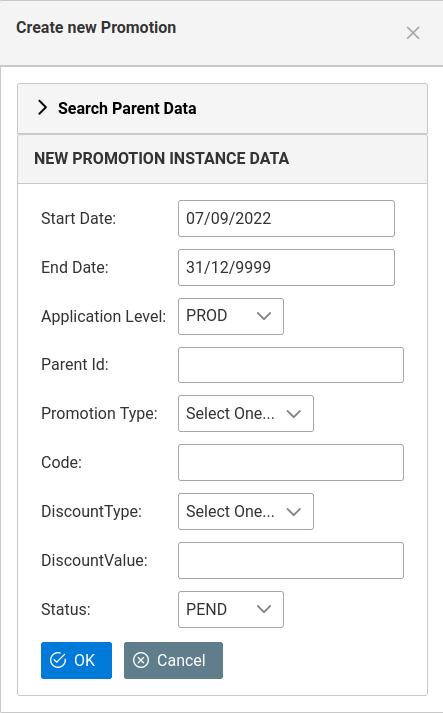
\includegraphics[width=\textwidth]{imaxes/formulario-alta-promocion-01.png}
    \caption{Sin el área de \emph{Search Parent Data} desplegada}
    \label{fig:formulario-alta-promocion-01}
  \end{subfigure}
%  \hspace{0.1\textwidth}
  \begin{subfigure}[b]{0.64\textwidth}
    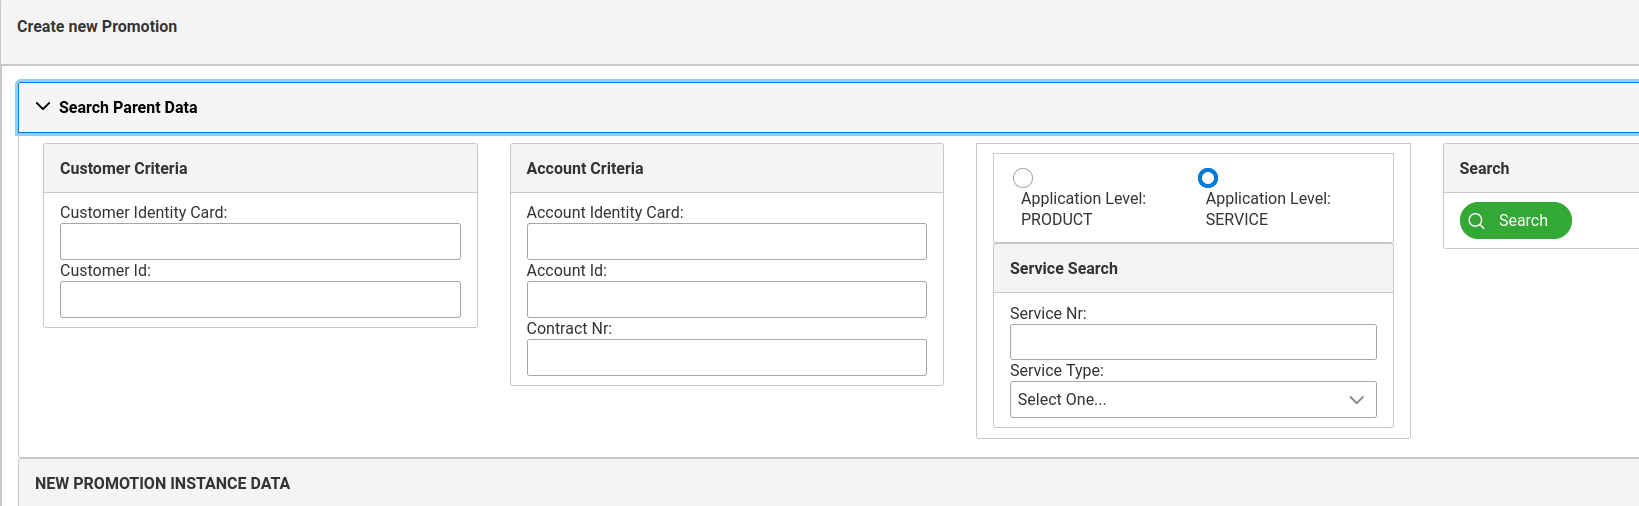
\includegraphics[width=\textwidth,height=3cm]{imaxes/formulario-alta-promocion-02.png}
    \caption{Con el área de \emph{Search Parent Data} desplegada}
    \label{fig:formulario-alta-promocion-02}
  \end{subfigure}
  \caption{Detalles del formulario de alta de promoción}
  \label{fig:alta-promocion}
\end{figure}


Una vez finaliza la introducción de datos se pulsará el botón \emph{OK} que confirma la operación del formulario de creación. Si todo es correcto se registra la promoción en el sistema y se muestran los datos de la promoción creado la pantalla de visualización de la entidad.

Por defecto la fecha de Activación de la promoción no se cubre, por lo que si queremos activar la promoción deberemos especificarla manualmente a través de la edición del registro de la promoción creada.

La \figurename~\ref{fig:alta-promocion} muestra dos detalles del formulario para añadir una nueva promoción, con y sin el \emph{Search Parent Data} desplegado.

\item[\underline{\textsl{\textbf{Editar registro de histórico de servicio}}}] Esta operación sólo está disponible para usuarios con permisos de edición.
Para editar un registro de histórico se seleccionará el registro deseado del listado de históricos de la entidad y se pulsará el botón editar de la columna \textit{EDIT ROW} correspondiente. Se editarán los campos pertinentes directamente en la tabla para realizar las modificaciones oportunas teniendo en servicio los criterios de fechas establecidos (definidos en la sección \ref{sub:histórico-conceptos} de la página \pageref{sub:histórico-conceptos}).

Al igual que para las entidades con históricos vistas en la sección del catálogo del sistema, si se cambia el estado de una promoción a cancelado, este cambio de estado se propagará a todos los registros posteriores al que cambiamos. Además se establecerá como fecha de cancelación la fecha en la que se realiza dicho cambio, propagándose ese dato por todos los registros de histórico de la promoción, no sólo los que están a continuación del registro al que se le cambió el estado a cancelado.

Esta propagación de la fecha de cancelación por todos los registros del histórico  también ocurre si se modifica dicha fecha. Lo mismo ocurre si se cambia la fecha de activación de la promoción.

\item[\underline{\textsl{\textbf{Añadir registro de histórico a una promoción}}}] Esta operación sólo está disponible para usuarios con permisos de edición.
Para añadir un nuevo registro de histórico sobre la promoción se seleccionará del listado el registro en el que se ubicará el nuevo registro a añadir y se pulsará el botón añadir de la columna \textit{ADD ROW} correspondiente. Aparecerá una nueva ventana emergente como la que se muestra en la operación de creación sin el área de búsqueda \emph{Parent Data} y con los campos cubiertos con la información del registro sobre el que se va a añadir el nuevo registro y se realizán las moficaciones oportunas sobre los mismos teniendo en servicio los criterios de fechas establecidos (definidos en la sección \ref{sub:histórico-conceptos} de la página \pageref{sub:histórico-conceptos}).

La \figurename~\ref{fig:nuevo-historico-promo} muestra un detalle del formulario para añadir un nuevo registro al histórico de una promoción:

\begin{figure}[H]
  \centering
  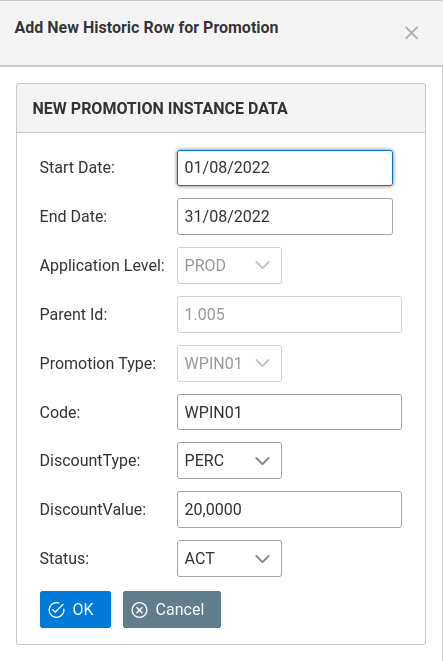
\includegraphics[width=0.45\textwidth]{imaxes/nuevo-historico-promocion.png}
  \caption{Detalle del formulario para añadir un nuevo registro de histórico de promoción}
  \label{fig:nuevo-historico-promo}
\end{figure}



\item[\underline{\textsl{\textbf{Borrar registro de histórico de la promoción}}}]
Esta operación sólo está disponible para usuarios con permisos de edición.
Para borrar un registro de histórico de la promoción se seleccionará del listado el registro a borrar y se pulsará el botón amarillo de borrar de la columna \textit{DEL ROW} correspondiente.

\item[\underline{\textsl{\textbf{Borrar la promoción}}}]
Esta operación sólo está disponible para usuarios con permisos de edición.
Para borrar completamente una promoción se deben borrar uno a uno todos los registros de histórico de la promoción según lo indicado en el punto anterior. 
\end{description}




\subsubsection{HIERARCHY - JERARQUÍA}

Para visualizar de forma simple y cómoda las distintas contrataciones existentes en el sistema se ha definido una vista de jerarquía de la misma. A la misma se accece a través del menú \emph{HIERARCHY} seleccionando la opción \emph{Hierarchy View} y muestra toda la información existente en el servicio para un cliente dado: sus cuentas asociadas así como los productos y servicios contratados para cada una de ellas junto a las cuotas y promociones que tienen asociadas.

Al acceder a esta pantalla se muestra un área de búsqueda, similar a las vistas en las entidades de contratación, con las siguientes áreas:
\begin{itemize}
	\item Área Account Data: en este área se definen los criterios de búsqueda relativos a una de las cuentas que pertenece al cliente a buscar:
		\begin{itemize}
			\item Contract Nr: número de contrato de la cuenta.
			\item Account Id: identificador de la cuenta.
			\item Account Identity Card: número del documento de identificación de la cuenta (NIF, NIE\dots).
		\end{itemize}
	\item Área Customer Data: en este área se definen los criterios de búsqueda del cliente.
		\begin{itemize}
			\item Customer Id: identificador del cliente.
			\item Identity Card: número del documento de identificación del cliente (NIF, NIE\dots).
		\end{itemize}
	\item Área Product Data: en este área se definen los criterios de búsqueda de alguno de los productos contratados por el cliente, para lo que se define el campo \emph{Product Id} correspondiente al identificador del producto.
	\item Área Service Data: en este área se definen los criterios de búsqueda de alguno de los servicios contratados por el cliente, para lo que se define el campo Service Nr: número del servicio a buscar.
	\item Área Search Date: fecha de referencia de búsqueda. Se obtendrá como resultado el registro de histórico en el que esté comprendida dicha fecha. Este campo es obligatorio para realizar la búsqueda.
\end{itemize}

Una vez cubiertos los criterios indicados se pulsará el botón \emph{Search}. Si existen clientes para los criterios definidos se mostrará un recuadro debajo del área \emph{Search Criteria} con un icono de usuario, tal y como se muestra en la \figurename~\ref{fig:vista-jerarquia-01}.

\begin{figure}
  \centering
  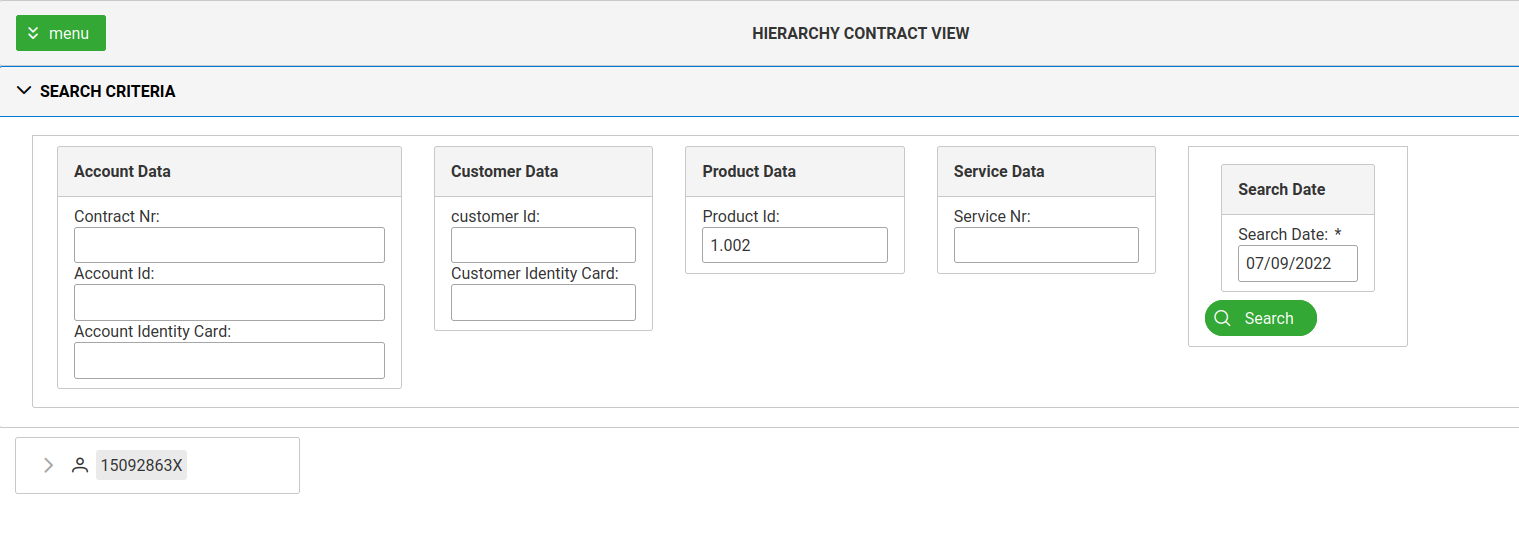
\includegraphics[width=\textwidth]{imaxes/vista-jerarquia-01.png}
  \caption{Detalle del resultado de la búsqueda del cliente para mostrar la jerarquía de contrataciones}
  \label{fig:vista-jerarquia-01}
\end{figure}

Pulsando en el símbolo \large{$>$} se despliega el nodo raiz correspondiente al cliente, y se van mostrando por niveles las distintas entidades de contratación que dependen del cliente: cuentas, productos contratados asociados a las cuentas, servicios, cuotas y promociones asociadas a los productos y cuotas y promociones asociadas a los servicios,  tal y como se muestra en la \figurename~\ref{fig:vista-jerarquia-desplegada}:


\begin{figure}[H]
  \centering
  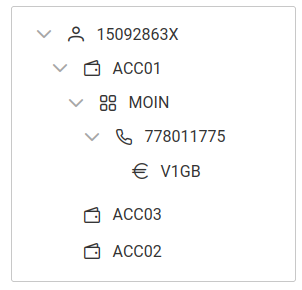
\includegraphics[width=0.35\textwidth]{imaxes/vista-jerarquia-desplegada.png}
  \caption{Detalle del resultado de la búsqueda del cliente para mostrar la jerarquía de contrataciones}
  \label{fig:vista-jerarquia-desplegada}
\end{figure}


Si pulsamos en cualquiera de los nodos se nos muestra la información relevante relativa a las distintas entidades que se situan sobre él en la jerarquía, así como la información de los históricos de la entidad correspondiente al nodo seleccionado, tal y como se puede ver en la \figurename~\ref{fig:vista-jerarquia-desplegada}.

\begin{figure}
  \centering
  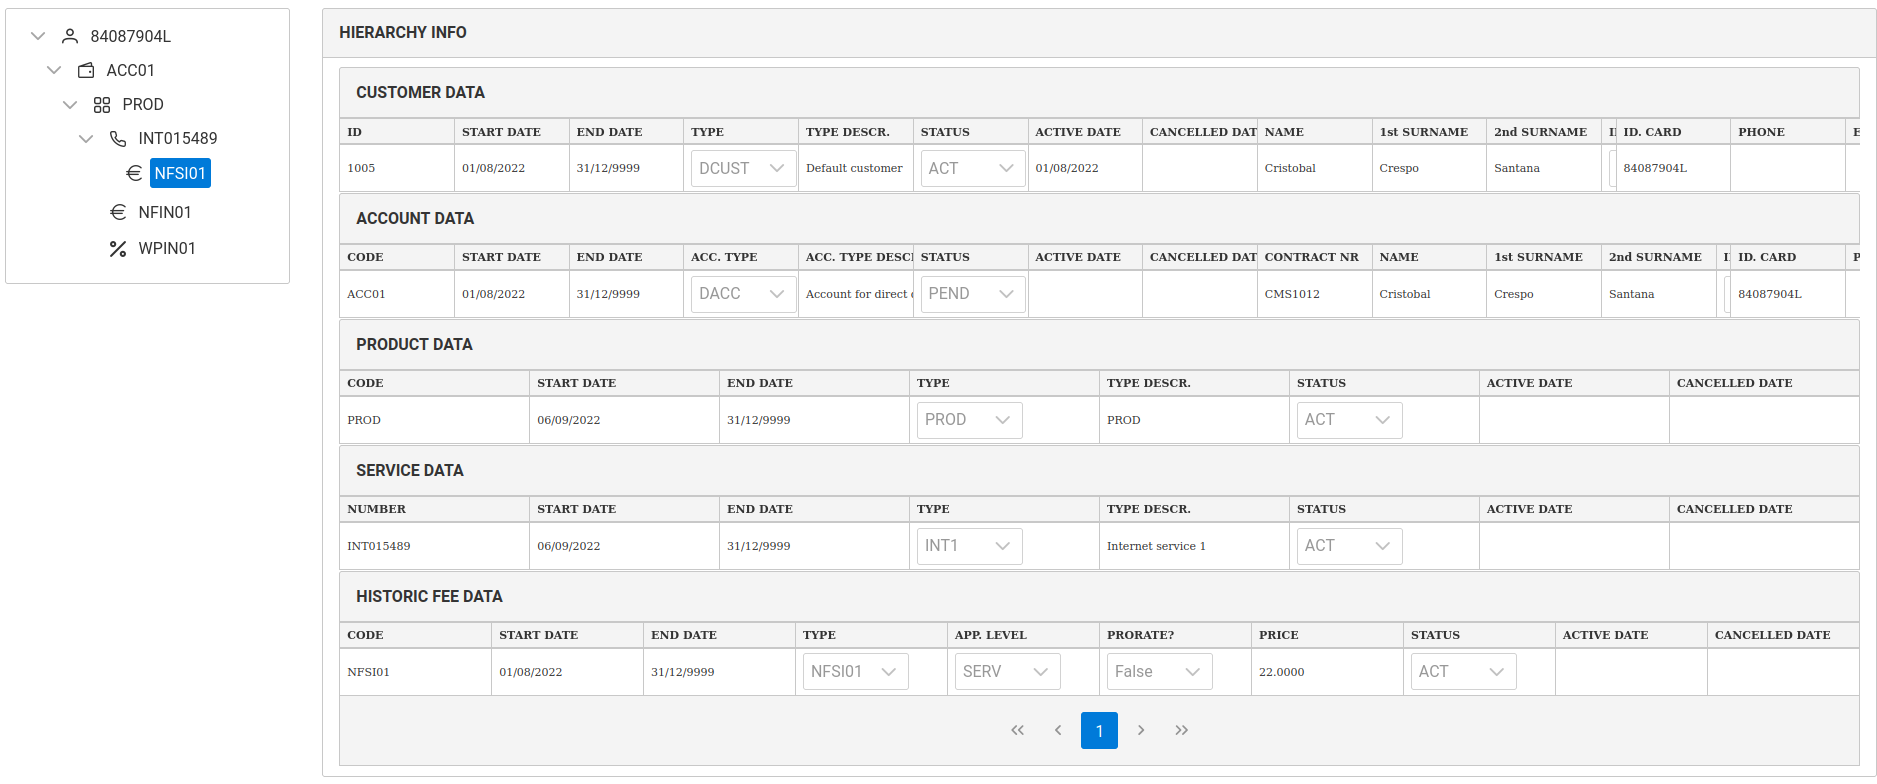
\includegraphics[width=\textwidth]{imaxes/vista-jearquia-informacion-nodo.png}
  \caption{Detalle de la información mostrada al seleccionar un nodo del arbol de jerarquía de contrataciones del cliente}
  \label{fig:vista-jearquia-informacion-nodo}
\end{figure}